\documentclass[a4paper,12pt,twoside]{book}
\usepackage[utf8]{inputenc}
\usepackage{dirtytalk}

% encodage
\usepackage{fontspec}

%avec overleaf, utiliser :
\usepackage[xetex]{hyperref}
\hypersetup{
pdfauthor = {Elsa Van Kote},
pdftitle = {titre},
pdfsubject = {Mémoire de stage portant sur la création du site Web Dyrin sous l'interface d'affichage XML MaX. Ce dernier est un outil développé par le Pôle document numérique de l'université de Caen. },
pdfkeywords = {PDN} {XML} {faune} {arctique} {MaX} {edition} {numerique} {Caen} {Dyrin}
}


%gérer les images%
\usepackage{graphicx}
\usepackage{caption}
\usepackage{subcaption}
\usepackage{float}
\usepackage[export]{adjustbox}
\usepackage{wrapfig}
\usepackage[english, french]{babel}
\graphicspath{ {./img/} }

\usepackage{minted}
\usepackage{csquotes}

% configurer le document selon les normes de l'école
\usepackage[margin=2.5cm]{geometry} %marges
\usepackage{setspace} % espacement qui permet ensuite de définir un interligne
\onehalfspacing % interligne de 1.5
\setlength\parindent{1cm} % indentation des paragraphes à 1 cm

\usepackage{lettrine} % lettrines (pas obligatoire)

%pour les notes référencées
\usepackage{footmisc}


%ajout des couleurs%
\usepackage{xcolor}
\usepackage{colortbl}


% Exemples de code : un grand merci à Kelly pour sa config !!
\usepackage{listings}
\usepackage{color}
\definecolor{codegray}{rgb}{0.5,0.5,0.5}
\definecolor{codepurple}{rgb}{0.58,0,0.82}
\definecolor{cyan}{rgb}{0.0,0.6,0.6}
\definecolor{codegreen}{rgb}{0,0.6,0}
\definecolor{backcolour}{rgb}{0.95,0.95,0.92}
\definecolor{lightgray}{rgb}{0.95, 0.95, 0.95}
\definecolor{darkgray}{rgb}{0.4, 0.4, 0.4}
\definecolor{purple}{rgb}{0.65, 0.12, 0.82}
\definecolor{editorGray}{rgb}{0.95, 0.95, 0.95}
\definecolor{editorOcher}{rgb}{1, 0.5, 0} % #FF7F00 -> rgb(239, 169, 0)
\definecolor{editorGreen}{rgb}{0, 0.5, 0} % #007C00 -> rgb(0, 124, 0)
\definecolor{orange}{rgb}{1,0.45,0.13}		
\definecolor{olive}{rgb}{0.17,0.59,0.20}
\definecolor{brown}{rgb}{0.69,0.31,0.31}
\definecolor{purple}{rgb}{0.38,0.18,0.81}
\definecolor{lightblue}{rgb}{0.1,0.57,0.7}
\definecolor{lightred}{rgb}{1,0.4,0.5}

% définition du langage XML
\lstdefinelanguage{XML}{
  backgroundcolor=\color{backcolour},  
  basicstyle=\ttfamily\footnotesize,
  morestring=[s]{"}{"},
  morecomment=[s]{?}{?},
  morecomment=[s]{!--}{--},
  commentstyle=\color{codegreen},
  moredelim=[s][\color{black}]{>}{<},
  moredelim=[s][\color{red}]{\ }{=},
  stringstyle=\color{blue},
  identifierstyle=\color{codegray},
  numberstyle=\tiny\color{codegray},
  breakatwhitespace=false,         
    breaklines=true,                 
    captionpos=b,                    
    keepspaces=true,                 
    numbers=left,                    
    numbersep=5pt,                  
    showspaces=false,                
    showstringspaces=false,
    showtabs=false,                  
    tabsize=2
}

% définition du langage JS
\lstdefinelanguage{JavaScript}{
  keywords={const, let, typeof, instanceof, new, true, false, catch, function, return, null, undefined, catch, switch, var, if, in, while, for, do, else, case, break},
  keywordstyle=\bfseries,
  ndkeywords={class, export, throw, import, this},
  ndkeywordstyle=\bfseries,
  sensitive=false,
  comment=[l]{//},
  morecomment=[s]{/*}{*/},
  commentstyle=\ttfamily,
  stringstyle=\color{blue}\ttfamily,
  morestring=[b]',
  morestring=[b]`,
  morestring=[b]"
}

%configuration des listes%
 \usepackage{enumitem}

%configuration de la mise en page : marges
\usepackage[margin=2.5cm]{geometry}

%insérer des chevrons%
\usepackage[T1]{fontenc}

\usepackage[automake,acronym,toc]{glossaries}
\makeglossaries

% gestion des acronymes %
\newacronym{METOPES}{METOPES}{Méthodes et outils pour l'édition structurée}
\newacronym{XML}{XML}{eXtensible markup language}
\newacronym{XSL}{XSL}{Extensible stylesheet language}
\newacronym{TEI}{TEI}{Text encoding initiative}
\newacronym{EAD}{EAD}{Encoded archival description}
\newacronym{AGEC}{AGEC}{Anti gaspillage pour une économie circulaire}
\newacronym{ADEME}{ADEME}{Agence de l'environnement et de la maîtrise de l'énergie}
\newacronym{CRAHAM}{CRAHAM}{Centre de recherches archéologiques et historiques anciennes et médiévales}
\newacronym{INR}{INR}{Institut du numérique responsable}
\newacronym{MaX}{MaX}{Moteur d'affichage XML}
\newacronym{CERTIC}{CERTIC}{Centre de ressources technologiques pour les TIC}
\newacronym{PDN}{PDN}{Pôle document numérique}
\newacronym{XSL-FO}{XSL-FO}{eXtensible stylesheet language - Formatting objects}
\newacronym{CPU}{CPU}{Central processing unit}
\newacronym{PUC}{PUC}{Presses universitaires de caen}
\newacronym{RAM}{RAM}{Random access memory}
\newacronym{MRSH}{MRSH}{Maison de recherche en sciences humaines}
\newacronym{DOI}{DOI}{Digital object identifier}
\newacronym{SGBD}{SGBD}{Système de gestion de base de données}
\newacronym{XXE}{XXE}{XMLmind XMLEditor}
\newacronym{PluCo}{PluCo}{Plugin Collaboratif}
\newacronym{DSI}{DSI}{Direction du service informatique}
\newacronym{SHS}{SHS}{Sciences humaines et sociales}
\newacronym{SGML}{SGML}{Standard generalized markup languages}
\newacronym{SEO}{SEO}{Search engine optimization}
\newacronym{WECG}{WECG}{WebExtensions community group}
\newacronym{W3C}{W3C}{World wide web consortium}
\newacronym{CECILL}{CECILL}{ CEa Cnrs Inria logiciel libre}
\newacronym{INRIA}{INRIA}{Institut national de recherche en informatique et en automatique}
\newacronym{CNRS}{CNRS}{Centre national de recherche scientifique}
\newacronym{BSD}{BSD}{Berkeley software distribution license}
\newacronym{DB}{DB}{Databases}
\newacronym{BVMSM}{BVMSM}{Bibliothèque virtuelle du mont Saint-Michel}
\newacronym{TLFI}{TLFI}{Trésor de la langue française informatisé}
\newacronym{FEW}{FEW}{Französisches etymologisches wörterbuch}
\newacronym{IIIF}{IIIF}{International image interoperability framework}
\newacronym{BNF}{BNF}{Bibliothèque nationale de France}
\newacronym{VIAF}{VIAF}{Virtual international authority file}
\newacronym{Cigref}{Cigref}{Club informatique des grandes entreprises françaises}
\newacronym{GES}{GES}{Gaz a effet de serre}
\newacronym{DHCC}{DHCC}{Digital humanities climate coalition}
\newacronym{svg}{svg}{Scalable vector graphics}
\newacronym{ITIS}{ITIS}{Integrated taxonomic information system}
\newacronym{ADW}{ADW}{Animal diversity web}
\newacronym{KPI}{KPI}{Key performance indicator}
\newacronym{PGD}{PGD}{Plateforme de gestion des données}
\newacronym{DOM}{DOM}{Document object model}
\newacronym{CSS}{CSS}{Cascading style sheets}
\newacronym{OGP}{OGP}{Open graph protocol}
\newacronym{MSH}{MSH}{Maison des sciences de l'homme}
\newacronym{TGIR}{TGIR}{Très grande infrastructure de recherche}
\newacronym{CLI}{CLI}{Commande ligne interface}
\newacronym{HTML}{HTML}{Hypertext markup language}
\newacronym{XPath}{XPath}{XML path language}

\usepackage[style=enc]{biblatex}
\addbibresource{biblio/memoire.bib}
\nocite{*}
\defbibnote{intro}{Cette bibliographie contient toutes les références utilisées pour le présent travail, par ordre alphabétique.}

\title{Mémoire de stage}
\author{E. F.}
\date{May 2022}



\begin{document}
\begin{titlepage}
		\begin{center}
			
			\bigskip
			
			\begin{large}				
				ÉCOLE NATIONALE DES CHARTES\\
				UNIVERSITÉ PARIS, SCIENCES \& LETTRES
			\end{large}
			\begin{center}\rule{2cm}{0.02cm}\end{center}
			
			\bigskip
			\bigskip
			\bigskip
			\begin{Large}
				\textbf{Elsa Van Kote}\\
			\end{Large}
		%selon le cas
			\begin{normalsize} \textit{licencié.e ès lettres}\\
				\textit{diplômé.e de master}
			\end{normalsize}
			
			\bigskip
			\bigskip
			\bigskip
			
			\begin{Huge}
				\textbf{Pratiques et réflexions autour de l'édition numérique de sources anciennes et de ses outils}\\
			\end{Huge}
			\bigskip
			\bigskip
			\begin{LARGE}
				\textbf{L'exemple du projet Dyrin, programme de recherche sur la faune du Grand Nord}\\
			\end{LARGE}
			
			\bigskip
			\bigskip
			\bigskip
			\begin{large}
			\end{large}
			\vfill
			
			\begin{large}
				Mémoire 
				pour le diplôme de master \\
				\og{} Technologies numériques appliquées à l'histoire \fg{} \\
				\bigskip
				2022
			\end{large}
			
		\end{center}
	\end{titlepage}

	\thispagestyle{empty}	
	\cleardoublepage
	
	\frontmatter
	\chapter{Résumé}
	\medskip
	Ce mémoire est le compte-rendu du travail mené au \acrfull{PDN} de l'université de Caen lors du stage de fin d'étude réalisé entre avril et fin juillet 2022. Il a consisté à la création du site Web du projet Dyrin portant sur les représentations de la faune arctique dans les oeuvres antiques, médiévales et modernes. Ce projet a été mené sous la responsabilité de Thierry Buquet, ingénieur de recherche au \acrfull{CRAHAM} et de Pierre-Yves Buard, ingénieur de recherche au \acrlong{PDN}. Le site Web consistait à une présentation de onze sources XML, chacune représentant un animal du Nord, appuyées par la création de plusieurs index.
	
	Une partie du travail consistait également à tester un nouvel outil développé par le \acrshort{PDN} et le \acrfull{CERTIC} : le moteur d'affichage XML prénommé MaX. Ce moteur d'affichage permet de créer des sorties HTML de ses données XML de manière autonome. Cependant il laisse également libre cours à une personnalisation des résultats à travers la manipulation de fichiers xQuery et XSL. Le site Web de Dyrin est ainsi le premier projet à être développé nativement sous MaX.
	
	Enfin, le dernier objectif de ce stage était également de comprendre les mécanismes de création d'une édition numérique de sources anciennes, ainsi que de développer un regard neuf et critique sur ces pratiques. \\
	
	\textbf{Dyrin} ; {PDN} ; {CRAHAM} ; {Caen} ; {edition} ; {recherche} ; {sciences-humaines} ; {FAIR} ; {environnement}
	
	\textbf{Informations bibliographiques~:} Elsa Van Kote, \textit{Titre du mémoire. Sous-titre du mémoire}, mémoire de master \og{}Technologies numériques appliquées à l'histoire\fg{}, dir. [Pierre-Yves Buard] [Thierry Buquet], École nationale des chartes, 2022.
	
	\chapter{Remerciements}
	
	\lettrine{M}es remerciements vont tout d'abord à toute l'équipe du \acrshort{PDN}, pour leur accueil chaleureux et leurs conseils si précieux.\\
	
	
	Ils vont aussi à M. Pierre-Yves Buard et M. Thierry Buquet pour m'avoir donné l'occasion de travailler sur ce beau projet.\\
	
	
	Également à Mme Lucence Ing, ma directrice de mémoire, pour son soutien et son indéniable talent de relectrice.\\
	
	
	À mon père, qui a été de si bons conseils.\\
	
	
	A mon mari, pour sa patience et toute son aide à la relecture.\\
	
	
	Et enfin à M. Thibault Clérice, directeur de notre Master, qui a su en l'espace de deux ans nous transmettre toute sa passion pour les humanités numériques\dots
	
	%bibliographie ici
	%\printbibliography
	
	\chapter{Introduction}
Si l'on devait expliquer le choix ayant motivé à faire ce stage, d'avril à fin juillet 2022, au sein du \acrfull{PDN} de l'université de Caen, il nous faudrait remonter à l'année 2018-2019. A ce moment là, alors en Erasmus à l'université d'Oslo, en Norvège, ce fut pour nous l'occasion de rédiger un mémoire de recherche portant sur les relations entre mères et enfants dans la Scandinavie du \textsc{xii}\ieme{} siècle. C'est à ce moment là que nous découvrions pour la première fois le monde des humanités numériques.

À notre retour en France, deux conclusions avaient été tirées : la première, qu'il était de notre désir de pouvoir mettre à profit les compétences historiques particulières développées lors de cette année (notamment l'apprentissage du norvégien, de la runologie et du vieux norrois\footnote{Le vieux norrois est la langue germanique du Nord de la Norvège médiévale, de l'Islande, du Danemark et de la Suède jusqu'au \textsc{xiv}\ieme{} siècle, d'où sont dérivées les langues scandinaves modernes.}). La seconde, que l'université d'Oslo offrait à ses étudiants des possibilités de savoirs historiques portés par le numérique au delà de tout ce que l'on aurait pu imaginer : un grand choix de ressources en provenance de bibliothèques, universités, bâtiments d'archives de toute la Norvège et du monde entier. Le tout accessible très facilement, rapidement, donnant accès à des sources d'une très haute qualité de définition, et offrant des possibilités de traitement, de recherche ainsi que de réutilisation considérables. Tel a été notre premier contact avec le domaine des humanités numériques. Nous ignorions alors à l'époque que la France n'avait pas non plus à rougir des moyens qui avaient été mis au service du numérique dans la recherche scientifique.

Ce n'est qu'en suivant le parcours du Master technologies numériques appliquées à l'histoire proposé par l'École des chartes que nous nous en sommes rendu compte. Dans un même temps, l'envie d'expérimenter ces humanités numériques devenait de plus en plus présente. C'est pourquoi il avait été décidé à l'issue de la première année de Master d'effectuer un stage de fin d'année, dans l'optique de parfaire des connaissances dans un premier temps très théoriques. Toujours curieuse de l'histoire de la Scandinavie et désireuse de travailler à nouveau sur des sources nordiques, nos recherches nous menèrent sur la page du projet Dyrin.

Dyrin n'est pas un acronyme : c'est un mot issu des langues scandinaves, le pluriel du mot islandais \og \textit{dyr} \fg, qui signifie \og animal \fg. Le projet Dyrin vise à la constitution d'un corpus de textes relatifs à la connaissance de la faune arctique et subarctique de l'Antiquité tardive jusqu'à 1600. L'axe principal du projet est la transmission des savoirs zoologiques sur cette faune encore mal connue avant les explorations de l'époque moderne. Le projet semblait en être encore à ses débuts, au stade du rassemblement de ressources scientifiques.
Après avoir pris contact avec le responsable de projet, l'ingénieur de recherche Thierry Buquet\footcite{buquet_thierry}, la proposition de stage fut acceptée. Ce premier stage eut lieu de mai à juillet 2021 au \acrfull{CRAHAM}. Il consista au dépouillement bibliographique de plusieurs ouvrages et mémoires sur la faune scandinave, ainsi que de nombreuses sources norroises, notamment des sagas. L'intégralité de ces données furent regroupées dans un fichier texte.

L'idée de faire un deuxième stage, cette fois-ci au \acrlong{PDN} de la \acrlong{MRSH} de Caen, bien qu'abordée dès 2021, n'a pas été une évidence. Le choix aurait pu se porter sur une institution ailleurs en France afin de découvrir d'autres pratiques. Cependant, nous tenions à faire notre stage au \acrshort{PDN} pour trois raisons différentes : la première, pour découvrir des méthodes de travail nouvelles. En effet les institutions du \acrshort{CRAHAM} et du \acrshort{PDN}, bien que toutes les deux situées au sein de l'université de Caen, et travaillant ensemble, ont cependant des objectifs et des pratiques scientifiques tout à fait différentes. La seconde raison étant que le \acrshort{PDN} était reconnu comme une institution pionnière de l'édition de sources numériques. Cette pratique d'édition permet la mise en lien et le partage de savoir scientifique à des fins de recherche et de développement. Elle s'appuie sur la publication d'oeuvres anciennes, d'articles scientifiques ou encore de ressources textuelles et iconographiques. Le monde de l'édition numérique s'est très vite emparée de la question de la représentation de la matérialité des sources, qui a été le point de départ de création du \acrshort{PDN} dix ans plus tôt. C'est un aspect qui nous semblait intéressant de découvrir. La troisième raison était notre désir de pouvoir suivre un projet depuis ses débuts jusqu'à la fin, c'est-à-dire depuis des données non structurées pour arriver à l'élaboration finale d'un site Web. Le projet Dyrin, sur lequel nous avions travaillé auparavant, nous semblait être l'occasion idéale.

Pour toutes ces raisons, le stage eu donc bien lieu au \acrshort{PDN} sous la direction de l'ingénieur de recherche Pierre-Yves Buard.

L'arrivée pour ce stage au \acrshort{PDN} a coïncidé avec la mise en ligne de MaX, un moteur d'affichage de fichiers XML développé par le \acrshort{PDN}. Après avoir mené une réflexion avec Pierre-Yves Buard et Thierry Buquet, plusieurs objectifs pour le stage furent établis.
Tout d'abord il fut décider de créer dans le temps imparti un premier état du site Web de Dyrin. Le second objectif du stage était de tester une prise en main autonome de MaX. En effet, bien que MaX ait été développé principalement pour les équipes de l'université de Caen, ses développeurs avaient également pour objectif de faire de MaX un outil utilisable par d'autres institutions de l'édition numérique. Il était donc important de savoir si la prise en main de MaX, aidé par une solide documentation, était réalisable pour des personnes extérieurs à l'université de Caen. Enfin, il a été de notre volonté de se donner comme objectif d'explorer à travers le projet Dyrin les impacts environnementaux liés à l'utilisation du numérique dans la recherche en sciences humaines et sociales.

Le stage ayant maintenant pris fin, nous pouvons nous demander quels liens avons nous pu faire entre ces trois objectifs distincts : En soit, de quelle manière le projet Dyrin, développé sous MaX, a été un espace d'apprentissage, de création et d'améliorations techniques, de même qu'un espace de réflexion autour des enjeux et des nouvelles pratiques des humanités numériques ?

Nous répondrons à cette question en étudiant dans un premier temps le fonctionnement des humanités numériques à l'université de Caen, reflet de l'interdépendance des institutions dans le monde de la recherche en sciences humaines. Puis nous détaillerons le fonctionnement de MaX entre innovation et questionnements autour des principes de la science ouverte. Enfin, dans un dernier temps, nous explorerons le développement du site Web de Dyrin en tant qu'espace propice aux explorations scientifiques et aux questionnements techniques concernant les humanités numériques de demain, notamment la question de leur empreinte environnementale.

	\thispagestyle{empty}
	\cleardoublepage
	
	\mainmatter 
 
 \part{Les institutions des humanités numériques à Caen}
 
\chapter{CRAHAM et histoire des savoirs zoologiques anciens : Dyrin et Ichtya}
    \section{Dyrin}
    Selon sa fiche de présentation sur le site du laboratoire \acrshort{CRAHAM}, le projet Dyrin a pour objet d'étude \og la connaissance de la faune spécifique du Grand Nord (régions arctique et subarctique), de l'Antiquité au \textsc{xvii}\ieme{} siècle, à travers la transmission des savoirs zoologiques (encyclopédies, etc.) et des pratiques humaines (chasse, pêche, commerce des matières animales)\fg.
    
   L'initiative du projet est venue de Thierry Buquet, ingénieur de recherche au \acrshort{CRAHAM}, et co-responsable du projet Ichtya\footcite{ichtya}. Plusieurs publications ont déjà fait part des problématiques scientifiques du projet Dyrin. Tout d'abord, la publication des actes du colloque de Cerisy-la-Salle en 2017 dont le thème était le suivant : \og \textit{Animaux aquatiques et monstres des mers septentrionales (imaginer, connaître, exploiter, de l'Antiquité à 1600)}\fg. Le compte rendu de ce colloque paru en 2018 dans la revue \textit{Anthropozoologica}\footcite{aquatique}, de même que l'introduction au volume, intitulée \og \textit{Pour une histoire des animaux aquatiques des mers septentrionales\footcite{natura}}\fg, traitait notamment des sources mentionnant cette faune arctique.
   
   Un autre article de Thierry Buquet, paru en 2020, portant sur \og \textit{Les informations relatives à la faune du Nord dans le Liber de natura rerum de Thomas de Cantimpré}\fg{} étudie la réception de quelques savoirs livresques et vernaculaires (et parfois tout à fait inédits) sur la faune scandinave dans une importante encyclopédie latine du \textsc{xiii}\ieme{} siècle dont les identifications zoologiques sont croisées puis comparées.
   
    \section{Ichtya}
   Dyrin est donc d'un projet porté de longue date par le \acrshort{CRAHAM} auquel participe activement la \acrfull{MRSH}. Loin d'être le premier projet monté entre ces deux institutions, Dyrin a su profiter des travaux réalisés pour de nombreux projets précédents, notamment pour le projet Ichtya. Ichtya est une bibliothèque rassemblant des textes latins consacrés à l'ichtyologie qui furent publiés dans l'Antiquité, au Moyen Âge et à la Renaissance\footcite{ichtya}. Il fut une des premières collaborations entre le \acrshort{CRAHAM} et le \acrshort{PDN}. Ce projet a permis notamment des
   réflexions sur la transmission et la structuration de savoirs anciens dans l'objectif de publier une bibliothèque numérique de textes latins de l'Antiquité à la fin du Moyen Âge\footcite{buquet_ichtya_nodate}.
   
   Ichtya a été un premier lieu propice à la réalisation d'un travail commun sur les modalités de représentation numérique des sources, de leurs apparats, des commentaires philologiques et zoologiques, en somme de la diversité des ouvrages dans leur provenance et leur intégrité, dont les typologies peuvent varier d'un auteur à un autre. De plus, ce projet, riche de son volume textuel de plus de 700 000 caractères \footnote{Ces textes sont rédigés par des auteurs aussi divers que Pline l'Ancien, Solin, Basile de Césarée, Ambroise de Milan, Isidore de Séville, Alexandre Neckam, Jacques de Vitry, Barthélemy l'Anglais, Vincent de Beauvais, Arnold de Saxe, Marc d'Orvieto, Pseudo-John Folsham, d'Albert le Grand et de Thomas de Cantimpré.} a abouti à la création avec les \acrfull{PUC} d'une édition papier: le livre IV du \textit{Hortus sanitatis} dont la partie \textit{ Tractatus de piscibus} (Traité sur les poissons) est un des huit traités qui le composent\footcite{noauthor_piscibus_nodate}. 
   
   L'histoire du projet Ichtya montre également la grande place faite au travail pluri-institutionnel au sein de l'université de Caen.
    
\chapter{Un travail collectif des institutions}
    La \acrshort{MRSH}, le \acrshort{CRAHAM}, le \acrshort{PDN} et les \acrshort{PUC}... C'est un aspect primordial de la vie de l'université : les institutions collaborent ensemble à la création de projets communs. Ces échanges sont particulièrement facilités par la très forte proximité géographique des différentes institutions, ce qui est d'une grande aide notamment pour les projets intra-universitaires. C'est dans le campus 1 de l'université que se trouvent, à moins de 150 mètres l'un de l'autre, le centre de recherche en histoire \acrshort{CRAHAM} et la \acrshort{MRSH} où sont logés les bureaux des \acrfull{PUC}, de l'infrastructure de recherche \acrshort{METOPES} et du \acrlong{PDN}. On trouve aussi à quelques pas la \acrfull{DSI} de l'université chargée notamment des développements d'outils de recherche plus lourds techniquement que ceux élaborés au \acrshort{PDN}. Un des grands enjeux de ces \og technopoles \fg{} de recherche est de faire de cette proximité un atout : il n'est en effet pas rare, même très anodin de voir les chercheurs et doctorants se déplacer en personne pour venir travailler avec les ingénieurs du \acrshort{PDN}. Des \og ateliers du \acrshort{PDN}\fg{} sont même organisés une fois par mois : il s'agit d'une après-midi réservée aux collaborateurs chercheurs, doctorants, qui sont autant de moments propices à la réflexion scientifique qu'au débugage de certains points techniques. 
    
    Dans le bâtiment de la \acrshort{MRSH} ce sont donc le \acrshort{PDN}, \acrshort{METOPES} et les \acrshort{PUC} qui se trouvent dans le même bâtiment, dans les bureaux mitoyens pour les uns (\acrshort{PDN}/Métopes), à l'étage inférieur pour les autres (\acrshort{PUC}).
    
    \begin{figure}[H]
        \centering
        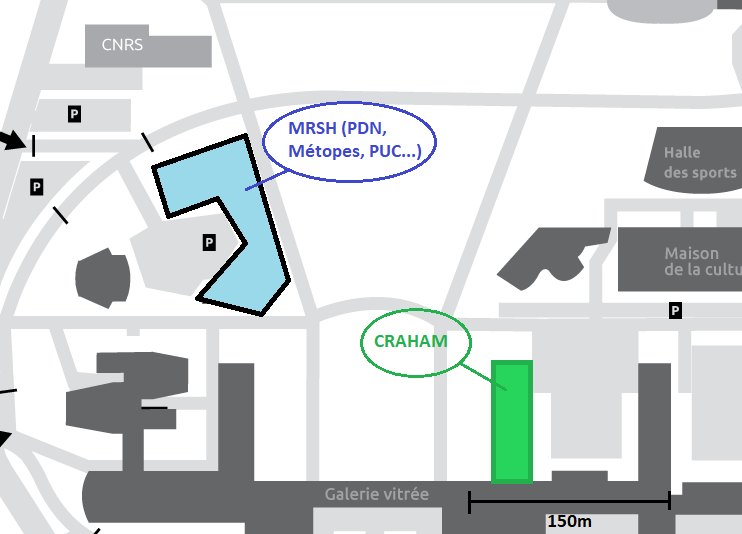
\includegraphics[width=10cm]{img/partie_1/campus-univ-zoom.png}
        \caption{Partie de plan du campus 1 de l'université de Caen où se situent à proximité la \acrshort{MRSH} et les laboratoires comme le CRAHAM.}
    \end{figure}
   
    
    \section{Le Centre de recherches archéologiques et historiques anciennes et médiévales médiévales (CRAHAM)}
    
    Au c\oe{}ur du Centre Michel de Boüard, dont le fondateur éponyme, Michel de Boüard (1909-1989), fut une grande figure de l'archéologie médiévale en France, est logé le laboratoire scientifique du CRAHAM. Créé dans la seconde moitié des années 1950, et homologué en 1959, la structure a d'abord réuni des archéologues, puis s'est ensuite ouverte aux historiens médiévistes, puis à ceux de l' Antiquité et aux spécialistes de langues et de littératures grecque et latine\footcite{craham}. Le bâtiment se situe sur l'esplanade du campus 1 de l'université de Caen. Le \acrshort{CRAHAM} abrite un ensemble de services exceptionnel pour une unité de recherche en \acrshort{SHS} : un laboratoire de paléoanthropologie, un laboratoire d'archéométrie-céramologie doté d'un matériel de caractérisation de haut niveau, un laboratoire de numismatique, un service d'archéomatique, un service d'édition et de communication ainsi qu'un service de dessin-cartographie. Le centre s'est doté également d'une belle bibliothèque de recherche spécialisée en archéologie et en histoire du Moyen Âge et conserve en son sein bon nombre de collections importantes en ostéologie et numismatique. Le \acrshort{CRAHAM} est notamment responsable de la publication de la revue \textit{Archéologie médiévale} et dirige la collection des \og Publications du Craham\fg{} éditée par les \acrlong{PUC}. Le \acrshort{CRAHAM} se compose d'environ 150 chercheurs et enseignants-chercheurs en histoire, archéologie, latin et grec, et il compte également dans sa structure de nombreux fonctionnaires ITA/BIATSS\footnote{ensemble de fonctions et de personnels de la Fonction publique composés de bibliothécaires, ingénieurs, personnel administratif et technique, du monde du social et de la santé.}, en plus de plusieurs doctorants\footcite{craham}.
    Le \acrshort{CRAHAM} s'implique fortement dans le domaine des humanités numériques : nombreux sont les projets ayant eu lieu en collaboration avec la \acrshort{MRSH}. Le centre a été moteur dans la création de \og plusieurs programmes de recherche dans l'édition multimodale de sources anciennes et médiévales documentaires (ex. du projet ANR Actépi) et littéraires (projet Ichtya), et pour la construction de bases de données textuelles, catalographiques, archéologiques et numismatiques (ex : Bibliothèque virtuelle du Mont Saint-Michel, Nummus…)\fg. Le \acrshort{CRAHAM} est aussi un des membres fondateur de l'Equipex Biblissima (2012-2019)\footnote{observatoire du patrimoine écrit du Moyen Âge et de la Renaissance, 2012-2021: \footcite{Biblissima}} ainsi que des consortiums CAHIER\footnote{consortium interdisciplinaire de projets numériques, en accès libre, menés principalement dans les domaines des \og corpus d'auteurs\fg, qu'ils relèvent de la littérature, de la philosophie ou d'une thématique liée à une école ou à une pratique: \footcite{consortium_cahier}}, COSME\footcite{consortium-cosme}, MASA\footcite{consortium-masa} de la \acrfull{TGIR} Huma-Num\footcite{huma-num}. Il participe désormais aux travaux de Biblissima+ (2021-2029)\footcite{Biblissima+}, ce qui peut souligner la reconnaissance de l'unité dans le domaine des humanités numériques.
    
    \section{Les Presses Universitaires de Caen (PUC)}
    
    Crées en 1984 comme service de l'université, les \acrshort{PUC} ont toujours comme mission principale de \og soutenir par leur savoir-faire l'édition et la valorisation de la recherche effectuée au sein des équipes caennaises et leurs réseaux nationaux ou internationaux\fg\footcite{PUC}. Elles travaillent en étroite collaboration avec des chercheurs de toutes disciplines et s'occupent également de la distribution des ouvrages publiés en dedans et en dehors de l'université. Bien que les \acrshort{PUC} publient en format papier, la manipulation et le travail effectué dès le stade numérique leur a permis de s'imposer dans le domaine des méthodes d'édition en contexte numérique comme peut en témoigner leur partenariat constant avec l'IR \acrshort{METOPES}.

    \section{Le Pôle Document Numérique (PDN)}
    
    Le Pôle Document Numérique est né de l'initiative de Julia Roger, ingénieure d'étude et actuelle directrice du \acrshort{PDN} et de Pierre-Yves Buard, ingénieur de recherche et ancien directeur du \acrshort{PDN}. À la fin des années 2010, alors qu'ils étaient employés aux \acrshort{PUC}, ils ont eu la volonté de développer un espace de travail et de recherche sur le traitement numérique des sources historiques. La thèse de Julia Roger, intitulée \og\textit{Descartes et ses livres. L'édition comme geste philosophique} \fg{} et soutenue en 2015, problématisait les exigences ainsi que les contraintes mise en lumière par l'édition papier, auxquelles étaient associées les possibilités offertes par la numérisation des manuscrits\footcite{roger_descartes_2015}. Pierre-Yves Buard soutenait sa thèse la même année, ayant pour intitulé \og \textit{Modélisation des sources anciennes et édition numérique} \fg{} et qui avait pour objectif d'essayer de définir des modèles d'édition spécifiques adaptés aux sources anciennes\footcite{buard_modelisation_2015}. Ces deux thèses ont donc en commun un travail de conceptualisation, de réflexion sur l'expressivité de la matérialité d'ouvrages à travers le numérique, et qui a donc été expérimenté les années qui suivirent. Dans un article de 2008 co-rédigé par Pierre-Yves Buard et Carole Dornier, une conclusion quant au rôle du numérique, alors encore très marginal, en avait-été tirée :  
    \begin{quote}
        Loin de faire obstacle à une version papier dont la relative pérennité et la maniabilité demeurent des atouts, ils [les outils numériques] peuvent être conçus en complémentarité : les introductions et notes savantes étant réservées à la version papier, l'exploitation et la valorisation du manuscrit dans ses aspects matériels constituent l'intérêt de la version électronique, utilisée aussi pour renvoyer à l'objet-livre\footcite{buard:hal-00322204}.
    \end{quote}
    Le numérique, notamment à travers l'utilisation de normes techniques, a permis d'éclaircir le rendu de la matérialité des livres, que l'édition papier peinait à retranscrire. C'est donc par cette porte de la matérialité de l'ouvrage que le numérique a pris sa place dans la \acrshort{MRSH} de Caen, pour ensuite s'étendre à d'autres enjeux et problématiques.

    \section{Méthodes et outils pour l'édition structurée (Métopes)}

    Dans les bureaux mitoyens à ceux du \acrshort{PDN} se trouve cette infrastructure de recherche conçue \og à l'usage des éditeurs et au service de l'activité éditoriale de l'ensemble des établissements publics d'enseignement supérieur et de recherche\footcite{Métopes}\fg. Soutenue par le CNRS, la chaîne Métopes est responsable de la création et du déploiement d'outils éditoriaux pour les éditeurs scientifique notamment via la création d'environnements de travail structurés et normés.
    
    Cette normalisation est essentielle afin de pouvoir remplir une autre des missions de l'infrastructure qui est d'assurer des fonctions de diffusion des produits éditoriaux, numériques ou imprimés en pleine connaissance des impératifs de l'idéal d'OpenAccess. Ces impératifs requièrent un travail conséquent sur la qualité de la donnée afin de pouvoir proposer des publications d'articles à des portails numériques tels OpenEdition\footnote{OpenEdition est un portail de ressources électroniques en sciences humaines et sociales.}, Cairn.info\footnote{Cairn.info est un portail web de revues et ouvrages en sciences humaines et sociales} ou encore Jats-NLM\footnote{Jats est une application qui définit un ensemble d'éléments et d'attributs XML pour le balisage et la description d'articles de revues.}, mais également pour du format papier. Une partie importante du temps de travail est également accordée à la formation d'éditeurs d'ouvrages numériques du monde scientifique. Ils sont plus de 400 à avoir été formés à ce jour\footcite{Métopes}.
    
    \section{Des méthodes de travail transversales nécessitant un dialogue constant}
    
     Toutes ces institutions, qui portent chacune des missions différentes, travaillent à l'aide d'un vocabulaire qui leur est propre. Lors de la réalisation d'un projet commun, un des plus gros enjeu est de parvenir à les faire se comprendre. L'élaboration d'un vocabulaire contrôlé et commun est une solution permettant à chacun d'exprimer de manière claire ses besoins et ses attentes.
     Bien que ces institutions soient géographiquement proches les unes des autres, ce travail est en réalité très complexe : il nécessite un dialogue constant entre les institutions, afin de s'assurer tout du long du projet que tout le monde parle bien de la même chose, et que chacun a conscience des objectifs des uns et des autres sur le long terme.
     Avant même le développement technique d'un projet, il est essentiel de prendre le temps de trouver ces termes, ces définitions à établir afin de pouvoir partir sur des fondations durables. 
     
     Si ces compétences de dialogue et de sensibilisation s'affinent au fil des projets, elles ne sont pas constamment gage de réussite. En effet, chaque projet possède son identité propre ainsi que des porteurs de projets différents. Les arguments apportés, de même que le lexique convenu ne sont donc jamais tout à fait les mêmes.
     Vis-à-vis du \acrshort{PDN}, il est donc important que ses ingénieurs aient une vision claire sur ce qui fait l'identité de leur institution, sur les enjeux et les missions qui lui sont confiées, afin de pouvoir les faire comprendre aux autres institutions.
     
     Par exemple, il arrive parfois que les entités \acrshort{PDN} et \acrshort{METOPES} soient confondues par des personnes extérieures, alors que les deux équipes n'ont pas du tout les mêmes missions\footnote{Pour rappel : le \acrshort{PDN} s'occupe du développement de projets numériques tels des bibliothèques et des bases de données, tandis que \acrshort{METOPES} est à la charge des publications d'articles dans des revues numériques scientifiques.}. Il revient dans ce cas là de bien redessiner les frontières de chacun afin de gagner en temps d'explication et en efficacité de travail. Il est particulièrement profitable dans ces cas là d'avoir avec soi des personnes issue des autres institutions : par exemple, deux anciens membres des \acrshort{PUC} travaillent au \acrshort{PDN}, et deux ingénieurs recrutés récemment ont travaillé plusieurs années au CRAHAM. Cela aide à l'élaboration de ce vocabulaire commun.
     
     
     Au tout début de la création du \acrshort{PDN}, il y a une dizaine d'années, un important travail de sensibilisation auprès des chercheurs avait été mené par les ingénieurs. L'objectif avait été de convaincre des personnes extérieures au monde de l'informatique de l'intérêt des outils numériques dans des projets de recherche. Malgré tous les projets menés par la suite, et après toutes ces années, ce travail de sensibilisation reste toujours le même. Même si, il faut le dire, les humanités numériques sont maintenant beaucoup mieux implantées dans le processus de recherche scientifique.
     
     Le but n'étant absolument pas de faire valoir une recherche qui passerait exclusivement par la voie du numérique. Il est tout à fait possible scientifiquement parlant, même en 2022, de ne pas avoir recours au numérique pour mener ses recherches. Il s'agit même d'un choix tout à fait défendable, le numérique ne devant être après tout qu'une valeur ajoutée et non une fin en soi. Cependant il est bon de rappeler que cette sensibilisation, qui passe par une explication claire des objectifs des institutions de recherche en numérique, sera toujours une part importante du travail de l'ingénieur.
     
     
     Une idée pour aider à cette sensibilisation avait été émise au \acrshort{PDN}. Il s'agissait de la réalisation d'une bibliographie informative sur l'identité et les missions de l'institution. Cette bibliographie, comportant divers articles rédigés notamment par Julia Roger et Pierre-Yves Buard, aurait permis aux nouveaux ingénieurs entrant au \acrshort{PDN} ainsi qu'aux autres institutions de mieux s'aligner avec les objectifs du \acrshort{PDN}. Toutefois cette bibliographie n'a pour l'instant pas encore vu le jour.
   

\chapter{Le laboratoire de recherche et d'édition de sources}
    Un des enjeux du \acrshort{PDN} par cette sensibilisation est de rappeler son rôle de laboratoire de recherche en édition de sources anciennes. Il est important de comprendre que le \acrshort{PDN} n'est pas un prestataire au service de l'université de Caen. Il s'agit d'une infrastructure de recherche, plus précisément :
    
    \begin{quote}
    (...) d'un groupe d'ingénierie inscrit dans une politique de recherche, déployant une activité de développement de projets en lien avec des équipes et des partenaires, ainsi qu'un espace de réflexion, de recherches interdisciplinaires, sur la méthode, les méthodologies du document numérique\footcite{noauthor_mrsh-pdn_nodate}.
    \end{quote}
    
Il ne s'agit pas de répondre simplement à des besoins et des demandes de chercheurs et ingénieurs extérieurs mais bien de proposer des nouvelles méthodologies et des solutions techniques après avoir mené une réflexion scientifique. Très soutenu par le \acrshort{CNRS}, actif et représenté dans de nombreux consortiums\footnote{CAHIER, MASA, Huma-Num...}, le \acrshort{PDN} a été un moteur dans la création de plus d'une soixantaine de projets à buts patrimoniaux mais également de recherche. De manière générale, le développement de projets porte trois objectifs principaux : premièrement, permettre aux chercheurs de mieux appréhender leurs données et de les voir sous un angle nouveau. Deuxièmement, le développement d'outils techniques par le \acrshort{PDN} et troisièmement, la diffusion du savoir dans l'espace public à des fins culturelles et scientifiques.

Cette culture scientifique de même que ces outils techniques peuvent ensuite être repris dans le futur par d'autres projets scientifiques. On peut alors se poser la question de l'accessibilité et la pérennité de ces projets : comment faire pour que ces derniers aient une véritable valeur scientifique alors que leurs donnés, leur structure de même que leurs aspects esthétiques évoluent lors de chaque mise-à-jour ? 
    
\section{L'édition papier comme pratique de stabilisation}

Pour répondre à cette question il faut se tourner vers les éditions papier. Bien que le \acrshort{PDN} soit chargé des projets d'édition numérique, il travaille toujours en étroite relation avec les \acrshort{PUC}. Chaque projet élaboré par le \acrshort{PDN} est ensuite édité en version papier, comme le montre la figure \ref{papier} ci-dessous pour les projets Malaterra et Ichtya.

  \begin{figure}[H]
    \centering
    \begin{subfigure}[b]{0.3\linewidth}
      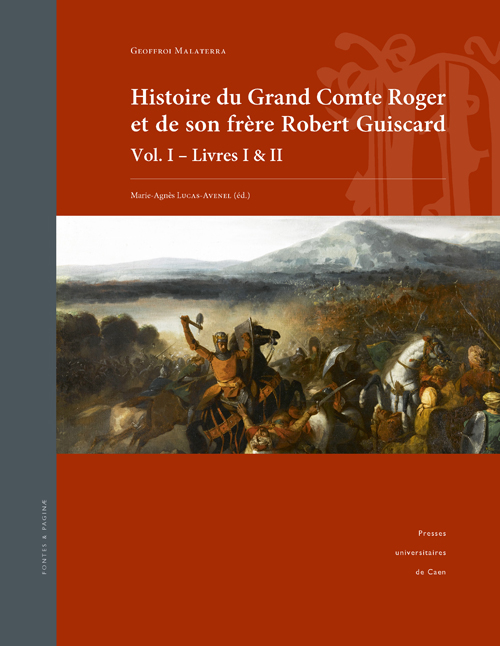
\includegraphics[width=\linewidth]{img/autre/couvMalaterra.jpg}
    \end{subfigure}
    \begin{subfigure}[b]{0.3\linewidth}
      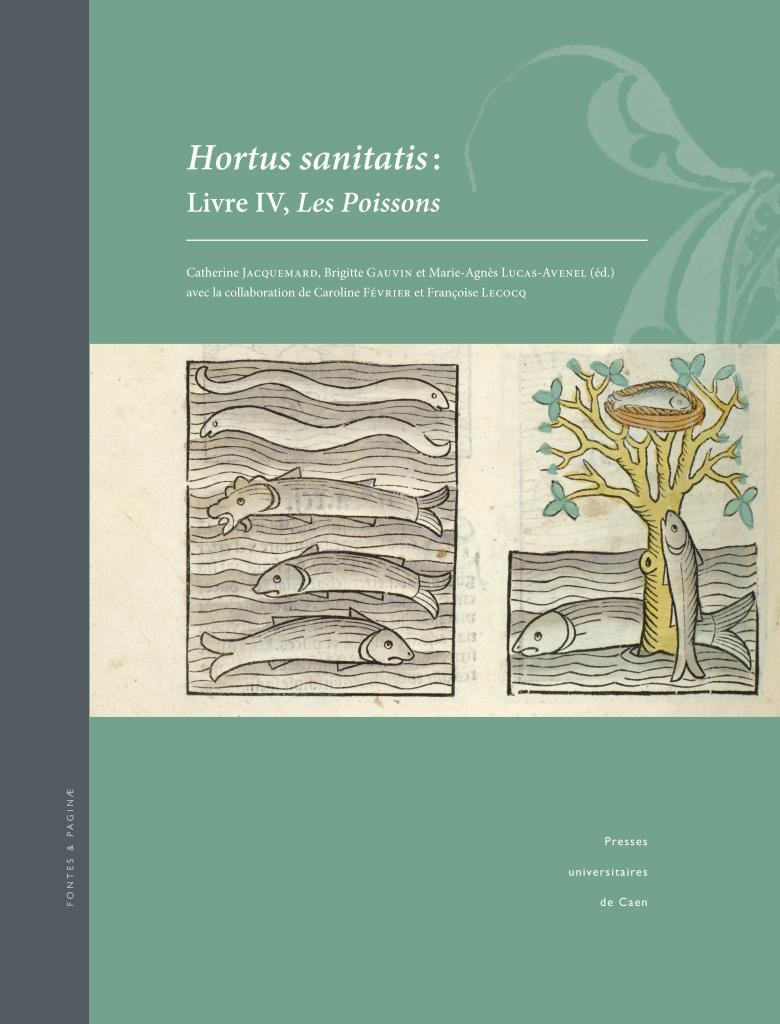
\includegraphics[width=\linewidth]{img/autre/depiscibus.jpg}
    \end{subfigure}
    \caption{À gauche, la couverture d'un des volumes de l'édition papier du projet Malaterra. À droite, celle d'un des volumes de l'édition papier du projet Ichtya.}
    \label{papier}
\end{figure}

Contrairement au monde du numérique, les éditions papier offrent la possibilité de rééditer des \oe{}uvres présentant des coquilles, des erreurs d'analyses ou des erreurs conséquentes de mise en page, tout en conservant l'\oe{}uvre précédente physiquement. Dans le monde de la recherche, l'arrivée du Web et du partage de connaissances de manière instantanée à l'échelle mondiale a non seulement fortement bouleversé les pratiques éditoriales papier, mais en a également, contrairement à ce que l'on pourrait penser, renforcé le rôle d'agent de contrôle.

En effet un des problèmes de l'ouverture de la recherche, et d'autant plus face à la forte expansion de la pratique de l'OpenData, pratique qui consiste à rendre accessible les données dont l'usage est laissé libre aux usagers, a été de ne plus y voir clair entre les recherches en cours, celles terminées, celles aux hypothèses validées ou bien rejetées. En somme, puisque la donnée est accessible à n'importe quel moment de la réflexion scientifique, cela peut porter à confusion pour un public inconscient des normes de la publication scientifique.

Dans les pratiques éditoriales universitaires papier, la publication d'un travail de recherche ne peut se faire sans être revue auparavant par des pairs, c'est-à-dire par un comité d'experts missionné dans le but de juger de la rigueur scientifique des hypothèses qui y sont développées. C'est une des fonctions principales des \acrshort{PUC} pour tout travail d'édition. Or, pour la recherche exposée via le numérique, en accès libre à tout instant, ce travail de vérification ne peut être effectué avant la diffusion des travaux. C'est pourquoi certains d'entre eux se retrouvent cités et partagés dans les journaux et les réseaux à des stades préliminaires, avec des pratiques scientifiques non validées parfois même erronées. Ce qui a évidemment d'importantes conséquences dans le débat public, car cela pourrait être apparenté à de la désinformation\footnote{La pratique de la désinformation peut être apparentée à l'ensemble de techniques de communication visant à tromper des personnes ou l'opinion publique pour protéger des intérêts (privés ou non) ou influencer l'opinion publique. Source : \cite{desinformation}}.

C'est le double jeu risqué de l'OpenData : faire de la transparence un gage de la rigueur scientifique mais qui peut être également se retourner contre elle-même et devenir, parfois sans le vouloir, source de désinformation.
     
    
 \section{L'outil Méduse : étape de statification des projets}
    
 Désirant offrir une solution indépendante du papier tout en restant sur des données numériques pour en délivrer l'accès, une solution a été développée au \acrshort{PDN} pour \og pétrifier \fg les données des sites web et ainsi empêcher toute modification. Cela a été rendu possible par l'intermédiaire du \acrfull{CERTIC}, qui est un département de la \acrfull{DSI} de l'université de Caen depuis 2015. Son personnel travaille à l'élaboration de technologies en collaborations avec les laboratoires, et c'est par ailleurs par cette enseigne qu'a été développé l'outil de statification de site-web Meduse.
    
    
Meduse est un outil en ligne de commande (\acrshort{CLI}) destiné à réaliser des copies statiques des projets du \acrshort{PDN}. L'intégralité des projets à disposition sur le site du \acrshort{PDN} sont en réalité des versions \og médusées \fg, dont les données ne peuvent plus bouger.

Pour télécharger Meduse, il faut avoir installé le langage de programmation python\footnote{Python est un langage de programmation OpenSource.}, de même que la commande \texttt{pip}\footnote{Pip est un gestionnaire de paquets utilisé pour installer et gérer des paquets écrits en Python.} afin de pouvoir lancer la commande \texttt{pip install meduse-CERTIC} dans son terminal. Une fois l'application téléchargée et le script lancé il suffit d'entrer la commande \texttt{./meduse mirror [lien du site] -d [chemin/pour/stocker/le/dossier]}  pour lancer la transformation statique du site en question. Le script va alors interroger tous les liens \acrshort{HTML} qu'il trouve sur le site en question et interpréter toutes les images de même que tous les fichiers croisés. Meduse va alors transformer toutes ces informations en fichiers et liens HTML qui pourront alors être ouverte sur n'importe quel navigateur.

Un fichier \texttt{wget.log} sert d'historique des transformations effectuées et nous donne des informations quant au fichier traité (date, emplacement, nom, futur emplacement...), notamment le poids final des pages Web. On peut voir que ce poids reste en général très léger (pas plus dizaine de ko par page), ce qui rend le transfert par mail ou autre très simple et rapide. Cette méthode a été utilisée pour partager une première version du site avec le responsable de projet, Dyrin n'étant pour l'instant pas accessible en ligne. Cela a permis au responsable de faire remonter toute une série de première modification sans avoir à se déplacer au \acrshort{PDN}.

Cette manière de figer le site et ses données permet par la suite de pouvoir l'intégrer au Web afin qu'il puisse servir de source pour d'autres projets par la suite.
   
   
    
    \chapter{Des choix conscients d'outils}
    Le \acrshort{PDN} est donc un laboratoire d'édition de sources anciennes ayant pour mission l'ouverture des données de la recherche en sciences humaines et sociales. Dans le cadre de cette volonté d'ouverture s'est posée la question des outils à utiliser. La tendance à la normalisation des pratiques (à entendre dans le sens de la production et de l'utilisation de normes) ont amené le \acrshort{PDN} à prendre plusieurs décisions, orientées sur quatre axes : la structuration de la donnée scientifique, le stockage, leur accès, leur exploitation et leur visualisation.
    
    \section{Structuration de la donnée scientifique : XML}
    
    Le \acrfull{XML} est langage à balises développé en  1998 et utilisé, entre autres, dans la conception des sites Web et pour faciliter les échanges d'informations sur Internet. Ce langage de description a pour mission de formaliser des données textuelles. Il s'agit, en quelque sorte, d'une version améliorée du langage HTML avec la création illimitée de nouvelles balises\footcite{def-xml}. Un exemple de ce langage est donné ci-dessous :
    
    \begin{minted}{XML}
    <?xml version="1.0"?>
        <tei:teiHeader>
            <tei:fileDesc>
                <tei:titleStmt>
                    <tei:title>Gerfaut</tei:title>
                    <tei:author xml:id="TBuquet">
                    <tei:name>Thierry Buquet</tei:name>
                    <tei:affiliation>CNRS, Centre Michel de Bouard-Craham UMR 6273,
                    Université de Caen Normandie</tei:affiliation>
                    </tei:author>
                </tei:titleStmt>
            <tei:publicationStmt>
    \end{minted}
    
    Le langage \acrshort{XML} est une des briques centrales au \acrshort{PDN}. Descendant du \acrfull{SGML}\footnote{langage de description à balises}, il en reprend les principes généraux. Un de ses principaux objectif est de faciliter l'interopérabilité des données. Parfaitement intégré aux \acrshort{PUC}, chez \acrshort{METOPES} et au \acrshort{PDN}, son intérêt principal est de permettre au chercheur d'annoter ses sources au fur et à mesure de leur découverte, sans a priori scientifique particulier. Le \acrshort{XML}, contrairement au \acrfull{SGBD} traditionnel, ne nécessite pas d'avoir un schéma pré-construit pour manipuler ses données, mais bien d'enrichir la source sans devoir penser et repenser des schémas de bases de données complexes.
    
    L'utilisation du \acrshort{XML} montre également un intérêt technique : ses possibilités de langage sont très larges, il est donc possible de dire beaucoup de choses avec ce langage. De plus, avoir des connaissances et des compétences en XML ouvre l'accès à une quantité d'outils d'exploitation importante, ce qui n'était pas encore le cas lors de sa mise en ligne une vingtaine d'années plus tôt. À cette époque alors, l'intérêt pour ce langage était réel, mais celui-ci n'était alors pas aussi développé et répandu qu'aujourd'hui.
    
    
   Un fait notable de ce langage est donc sa grande diffusion. Pour citer quelques exemples, \textit{LibreOffice} manipule ses données en \acrshort{XML}, l'extension \texttt{.odt} est un fichier \texttt{.zip} dans lequel on trouve des fichiers en \acrshort{XML}. La lettre \og x \fg{} de \texttt{.docx} fait référence au \acrshort{XML}, avec toutes ses variables qui suivent... Tous ces outils fonctionnent avec du XML.
   
   Dans le domaine de l'édition scientifique on retrouve également cette technologie XML. Les \acrshort{PUC} utilisent par exemple le logiciel \textit{InDesign} sur la base d'un import \acrshort{XML} qui, d'un côté, permet la production d'un site Web, et de l'autre, la production d'une forme imprimée avec une mise en page relativement complexe propre aux publications scientifiques.
    
    Ce n'est cependant pas ses caractéristiques de langage à balise qui font, du point de vue du \acrshort{PDN}, l'intérêt essentiel d'\acrshort{XML} mais plutôt sa structure arborescente. Cet intérêt se situe dans la localisation \og spatiale \fg{} des éléments à l'intérieur d'un même arbre comportant un certains nombre de branches qui se développent, représentant des chapitres, des parties, des sections... Il n'est plus question de simples balises mais bien de toute une structure dont les éléments, classés en différents groupes, sont inter-dépendants les uns aux autres.
    
   \acrshort{XML} est au centre des technologies utilisées par le \acrshort{PDN}. L'idée est de partir de données non structurées que l'on va par la suite ramener à des vocabulaires contrôlés \acrshort{TEI} (\acrlong{TEI}) et \acrshort{EAD} (\acrlong{EAD}). Cela va permettre une structuration fine des données imbriquées les unes dans les autres. Tout au long de ce travail d'annotation, il est important d'essayer de factoriser au maximum les informations entrées afin d'éviter leur répétition au sein du fichier XML. L'avantage d'une telle factorisation est un gain de temps dans le futur traitement de cette donnée XML. Ce traitement pourra se faire lors de la mutualisation des données dans des bases locales d'autorité dédiées. C'est ce qui a été fait par exemple avec les bases Thesauri\footnote{Pour plus d'informations voir la partie sur les Thesauri en \ref{thesauri}} du \acrshort{PDN} : ces bases regroupent de manière collective et collaborative des données XML en provenance non plus d'une source unique, mais de tout un ensemble de sources produites par les chercheurs et ingénieurs de l'université de Caen.
   
   Au \acrshort{PDN}, deux langages XML sont utilisés : d'une part l'\acrshort{EAD} devenu un format de catalogage courant pour la description des fonds d'archives et des manuscrits, aussi bien dans les services d'archives que dans les bibliothèques. On retrouve cette forme de langage au \acrshort{PDN} dans des projets comme la \acrfull{BVMSM}\footnote{Consultable à cette adresse : https://emmsm.unicaen.fr/emmsm/bvmsm/accueil.html}). De l'autre, le langage TEI pour de l'édition de sources textuelles, utilisé pour des projets comme Ichtya. Dans les deux cas, l'utilisation de ces langages nécessitent la création d'un vocabulaire contrôlé.
   
   Au \acrshort{PDN}, une partie importante du travail est dédiée au choix de dénomination de ce vocabulaire, c'est-à-dire de ces parties du texte que l'on trouve dans les \oe{}uvres physiques : apparat critique, annotation de l'auteur, annotation de bas de page ou bien encore notes en marge. Ce choix est pris en concertation entre ingénieurs et chercheurs.
   
   Si l'\acrshort{EAD} permet une liberté d'annotation, cela est d'autant plus vrai pour la \acrshort{TEI} : ce langage est doté d'un grand nombre de modules, d'éléments et d'attributs offre une grand liberté d'annotation. Malgré tout, ce vocabulaire reste contrôlé, notamment pas la publication de Guidelines\footnote{Les Guidelines sont de la documentation concernant les règles de structuration TEI. \cite{guidelines}}. Ce qui peut amener certains chercheurs à exprimer leurs doutes quant à l'utilisation de la TEI pour la description de sources, estimant que malgré cette liberté d'annotation, la \acrshort{TEI} reste tout de même contrainte dans un cadre déjà fixé à l'avance, limitant ainsi la réflexion scientifique possible.
   
   Si le \acrshort{PDN} a fait le choix de l'\acrshort{XML}, a aucun moment il n'en impose son utilisation à ses partenaires. Le fait, pour certaines institutions, de ne pas souhaiter utiliser la \acrshort{TEI} de nos jours pour structurer les textes, est une décision à respecter, mais qui reste cependant à argumenter : se passer de la \acrshort{TEI} c'est se passer de 40 ans de réflexions, de recherche et de développement sur les objets que constituent les textes. Pour preuve, ce langage existe depuis 1986 et existait bien avant \acrshort{XML}.
   
   Cette dernière technologie est une brique technique qui peut être appelée à changer, contrairement à la \acrshort{TEI} et \acrshort{EAD} qui sont des vocabulaires solides et bien implantés, d'où l'importance des standards : ils surplombent celle des aspects techniques, leur permettant de durer dans le temps.
   
    \section{L'importance de questionner nos habitudes techniques}
    
    Ces briques \acrshort{XML},\acrshort{TEI} et \acrshort{EAD} sont utilisées pour modéliser les données à l'intérieur d'environnements de travail, dont on trouve un exemple en figure \ref{envi}. Ces derniers sont des interfaces créées pour faciliter le travail et les interactions entre le chercheur et l'arbre XML en devenir. Cette notion d'environnement provient de l'éditeur XML \acrfull{XXE} de la société française Pixware\footcite{pixware} qui a été choisi au \acrshort{PDN}, au début des années 2000, pour diverses raisons que nous allons détailler.
    
    \begin{figure}[H]
    \centering
    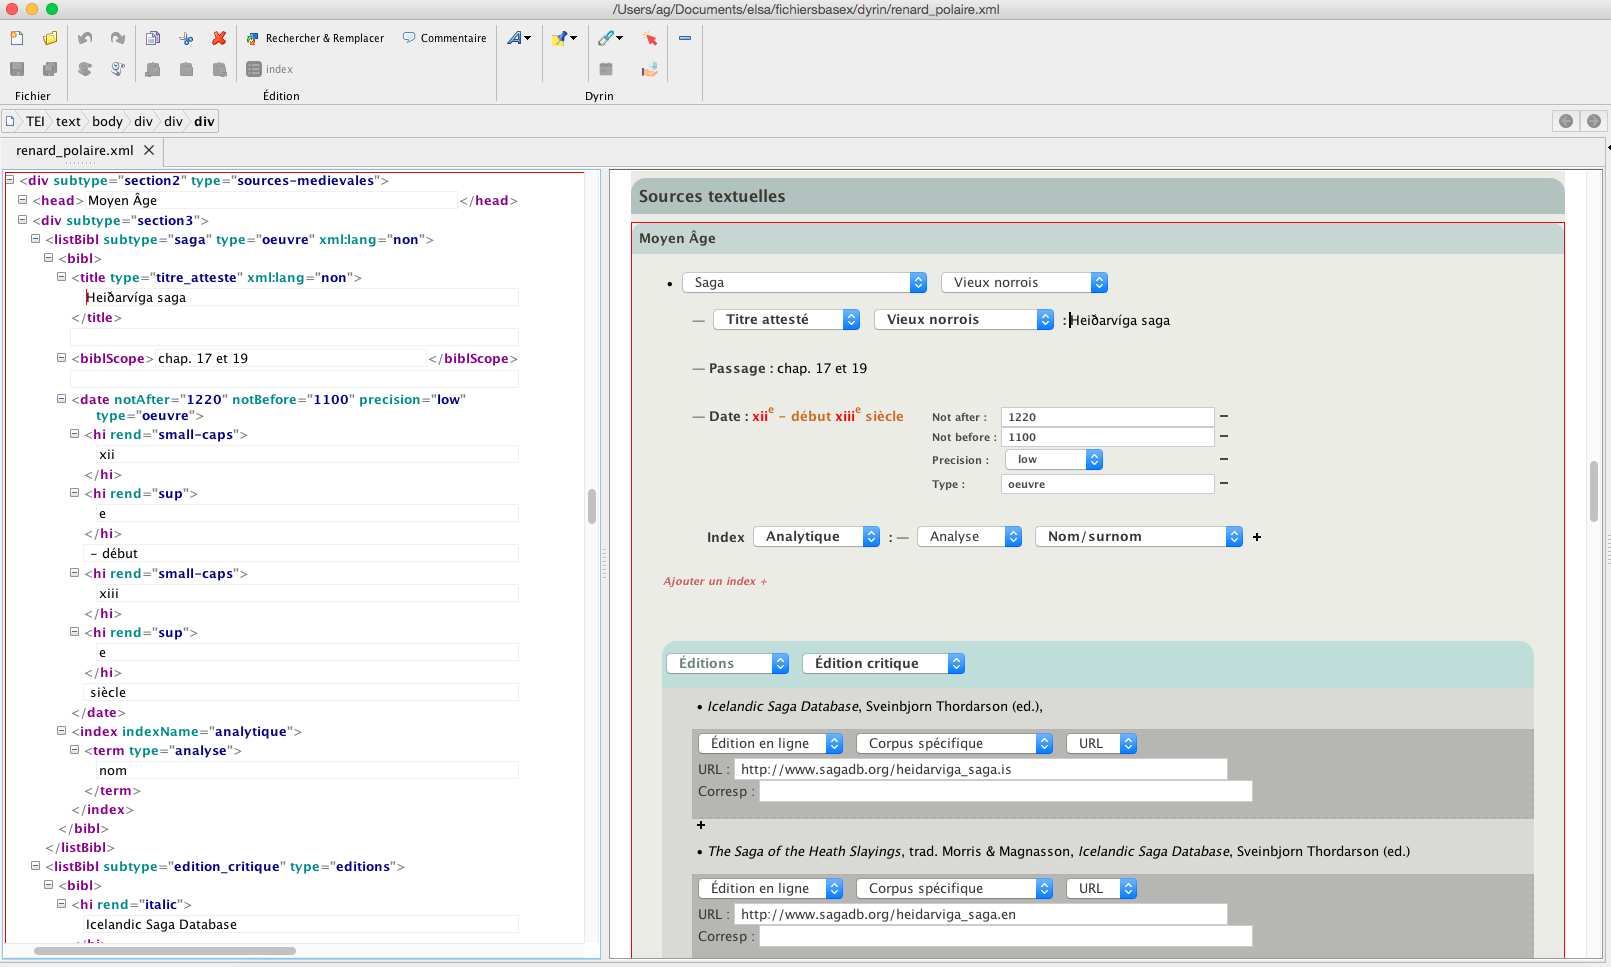
\includegraphics[width=12cm]{img/MaX/env_interface.png}
    \caption{Capture de l'interface de XXE : à gauche l'arbre XML et au centre l'environnement de travail créé pour Dyrin.}
    \label{envi}
\end{figure}
    
    
    Comme nous venons de le dire, il est essentiel de considérer les documents \acrshort{XML} comme des arbres. Il a donc été décidé au \acrshort{PDN} de chercher un éditeur d'arbre et non pas un éditeur de code. Le très connu logiciel Oxygen XML Editor\footcite{oxygen} n'a donc pas été retenu, étant considéré comme un éditeur de code \acrshort{XML}. Il s'agit en effet d'un très bon environnement de développement de technologie \acrshort{XML} qui offre la possibilité d'annoter une source, de développer des feuilles de transformation \acrshort{XSL}, de même que d'y incorporer ses propres requêtes xQuery\footnote{xQuery est un langage de requête informatique permettant non seulement d'extraire des informations d'un document XML, ou d'une collection de documents XML, mais également d'effectuer des calculs complexes à partir des informations extraites et de reconstruire de nouveaux documents ou fragments XML (\cite{xquery}). Nous y reviendrons plus en détails dans la partie \ref{que}.}. Cependant ses fonctionnalités ne sont pas adaptées à tous les utilisateurs en ce qui concerne l'édition numérique.
    
    Il est vrai que lorsque l'on est chercheur, nos enjeux et nos objectifs de travail ne sont pas les mêmes que ceux d'un ingénieur. Il n'est pas du ressort du chercheur de construire des feuilles de transformations \acrshort{XSL} ou bien d'élaborer des requêtes xQuery. Le chercheur est celui devant apporter avant tout son expertise scientifique. La technique reste le travail de l'ingénieur. C'est ce genre de réflexion qui a présidé le choix d'\acrshort{XXE} au \acrshort{PDN}.
    
    Quelques années auparavant, le projet \textit{Hortus Sanitatis} avait servi de premier cadre de réflexion menée sur le meilleur outil à utiliser : un outil le moins lourd possible, peu technique, mais qui permettent aussi une annotation en TEI. L'objectif était le développement d'un outil façon WYSIWYG\footnote{Littéralement : \textit{What You See Is What You Get}} qui permettait, tout en annotant ses sources, de pouvoir surveiller en continu la création de l'arbre XML correspondant. Cet outil permettrait également la multiplication des vues adaptées à la tâche actuelle du chercheur : transcription, annotation de diverses natures, d'indexation...tous ces moments d'annotation du texte correspondent à des interfaces de travail particuliers. C'est à ce moment que le choix d'\acrshort{XXE} fut pris.
    
    À travers l'interface XXE, le chercheur, maîtrisant l'annotation, a accès à l'arbre \acrshort{XML} dont il contrôle le schéma mis en place. Toutes les contraintes techniques (conformité des balises, du schéma) étant prises en charge par le logiciel. L'outil parfait techniquement n'existant pas, il faut toutefois que le chercheur contrôle visuellement la construction de son arbre XML afin de repérer d'éventuels chevauchements ou déplacements de balises incongrus.
    
    Cette question du choix des outils est primordiale. Le choix d'XXE a été porté par une réflexion autour des tâches et des missions attribués à chacun, dans l'optique de trouver l'outil le plus adapté. Chaque décision a un impact et des coûts réels sur plusieurs plans : un coût financier, tout d'abord, car le choix de tel ou tel outil n'est pas sans conséquences d'un point de vue budgétaire. Des outils comme Oxygen ou bien XXE sont accessibles dans leur version professionnelles via des licences payantes. Cependant seul XXE propose une version gratuite à usage personnel pour des projets à but non lucratif. Une des prochaines étapes de réflexion serait peut-être de chercher un logiciel OpenSource, c'est-à-dire un logiciel dont le code est ouvert au public. Un logiciel OpenSource repose sur la révision par les pairs et par les contributions des communautés de programmeurs. Un de ses grand avantages est sa grande flexibilité permettant d'ajuster le logiciel à des besoins spécifiques sans autorisation d'un fournisseur.
    
    
    Le numérique, par sa croissance exponentielle dans la recherche en SHS, ne peut être analysé à l'échelle individuelle. Il doit se comprendre comme une cause aux conséquences multiples, à une échelle démesurément plus grande que celle de l'individu. Au \acrshort{PDN}, c'est plus de soixante projets qui ont vu le jour, sur lesquels on travaillé des dizaines de chercheurs et ingénieurs. Il est donc important de réfléchir à l'outil dans son utilisation avant de le déployer à grande échelle : dans notre cas, le chercheur n'est pas ingénieur, il n'a donc pas à devoir s'inquiéter des aspects techniques numériques. C'est pourquoi il nous semble qu'un outil comme Oxygen n'est pas la meilleure option, car il donne au chercheur des missions techniques (ouverture, fermeture des balises...) dont il ne devrait pas avoir la charge. \acrshort{XXE} quant à lui, est un meilleur parti en correspondant mieux au travail demandé au chercheur : annoter simplement un arbre \acrshort{XML} à travers une interface graphique pensée sur mesure.
    
    Cette question doit aussi se poser du point de vue de l'ingénieur : il est selon nous de son devoir de trouver les outils adaptés à la tâche de chacun. Le choix d'un outil doit être fait en fonction de son utilité et de son utilisateur, afin de pouvoir tirer un maximum de ses potentialités et éviter la situation que formulait Abraham Maslow en 1966 : \og Je suppose qu'il est tentant, si le seul outil dont vous disposez est un marteau, de tout traiter comme s'il s'agissait d'un clou.\fg
    
    En ce qui concerne les langages XML-TEI et EAD, ce qui fait la force de leur utilisation via l'éditeur XXE est à la fois de permettre l'interopérabilité des données entre collaborateurs et également une personnalisation de leur modélisation.
    
    \section{La question du stockage: BaseX\label{basex}}
    
    La question du stockage des données a été très problématique jusqu'au début des années 2000. À cette époque ces fichiers \acrshort{XML} devaient être stockés de la même manière que les fichiers d'autres formats sur des disques durs de serveurs, posant inévitablement des problèmes d'efficacité en terme d'accès, de possibilité de requêtages, de sécurité, etc... Mais cela a pris fin à partir du moment où il a été possible de disposer de bases de données natives \acrshort{XML}. En effet, l'arrivée d'eXist ainsi que le développement à maturité d'eXist-db à permis des solutions de stockage intéressantes. 
    
    \begin{wrapfigure}{r}{0.25\textwidth}
    \centering
    
\includegraphics[width=0.25\textwidth]{img/partie_1/existdb.jpg}
    \caption{Logo du système de gestion de base de données eXist.}
\end{wrapfigure}
    
    
    Au \acrshort{PDN}, le choix avait été fait il y a quelques années d'utiliser un logiciel de base de données \acrshort{XML} natif intitulé BaseX. À l'époque où ce choix avait été fait, et où la question se posait entre la technologie BaseX ou bien eXist-db, BaseX se montrait beaucoup plus stable sur le plan technique. Certes eXist était très rapide et très efficace sur de petites quantité de données, beaucoup plus que BaseX, mais l'outil posait des problèmes de stabilité criants, qui rendait incontournable le redémarrage des serveurs une fois par semaine. Cependant, si cela était vrai avec les premières versions d'eXist, il serait intéressant de refaire les tests de performance effectués des années plus tôt, les dernières versions du logiciel étant beaucoup plus stables. 
    
    Les équipes d'ingénieurs du \acrshort{PDN} sont après toutes ces années habitués à cette technologie. Cependant, comme nous le faisions remarquer un peu plus haut, l'habitude n'exclue pas la réflexion. BaseX étant une brique outil, celle-ci pourra très bien être changée en temps voulu si les circonstances le veulent. Jusqu'à ce jour, BaseX reste très fonctionnel pour les tâches accomplies au \acrshort{PDN}. Il faut également noter que les outils actuellement développés, c'est le cas notamment de MaX, le sont sous cette technologie. Changer cette dernière reviendrait à reprendre l'intégralité des développements et ne pourra pas se faire du jour au lendemain.
    
     \begin{wrapfigure}{l}{0.25\textwidth}
    \centering
    
\includegraphics[width=0.20\textwidth]{img/partie_1/baseX.png}
    \caption{Logo du système de gestion de base de données BaseX.}
\end{wrapfigure}
         Un des grands intérêts de BaseX est sa politique d'utilisation : il s'agit d'un logiciel gratuit, ce qui n'est pas négligeable. De plus il s'agit d'un logiciel OpenSource\footnote{"BaseX is completely OpenSource." \cite{map_xml}} dont les mises-à-jour sont apportées par une communauté très active. BaseX porte en lui deux modes de fonctionnement :
         
    Le premier est un mode client, BaseX-GUI (Graphical User Interface), c'est-à-dire un logiciel que l'on peut lancer sur l'ordinateur pour tester des requêtes à travers un interpréteur de langage xQuery très puissant. C'est une fonction beaucoup utilisée au \acrshort{PDN} notamment par les doctorants dans le cadre de leurs travaux de thèse. Ce mode client reste très commode car il requiert simplement de télécharger BaseX, de créer une base de données de documents XML, puis de rédiger dans l'interface la commande xQuery souhaitée. Le logiciel envoie ensuite le résultat sous forme d'arbre XML.
    
  
    Si l'on souhaite avoir accès à l'espace client de BaseX il faut lancer le script du fichier \texttt{basexgui} qui va lancer l'application.
    
    \begin{figure}[H]
    \centering
    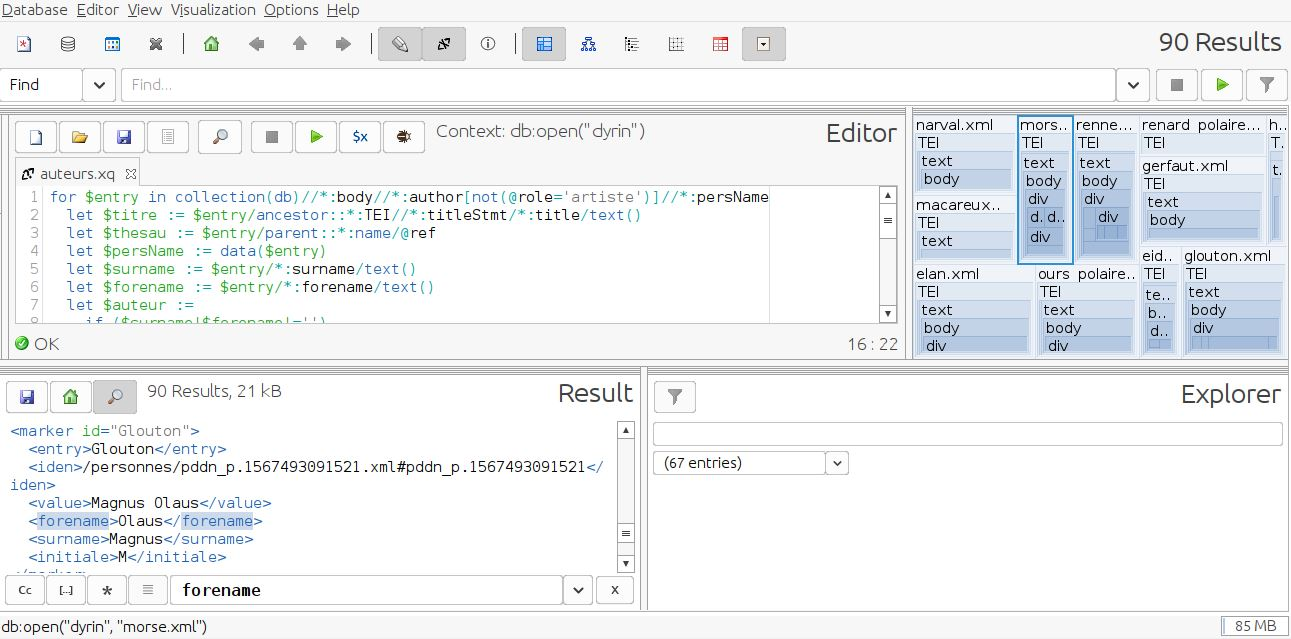
\includegraphics[width=14cm]{img/partie_1/basex_interface_client.JPG}
    \caption{Capture de l'interface client de BaseX.}
\end{figure}
    
    La figure ci-dessus est une capture de l'interface client BaseX. On peut voir sur la droite en bleu les onze fichiers de la base de données Dyrin. À gauche une requête en langage xQuery permet d'aller chercher tous les auteurs d'\oe{}uvres présents dans toutes les fiches animales. Enfin, en bas à gauche se trouve une partie du résultat de cette requête où apparaît le nom d'Olaus Magnus, un des auteurs présents dans la fiche sur le glouton. BaseX offre la possibilité de pouvoir sauvegarder sa requête en format \texttt{.xq} ainsi que le fichier de résultats de sortie sous format XML. Le résultat est visible ci-dessous en figure \ref{xq-auteurs} et \ref{xml-auteurs}.
    Cette possibilité  d'enregistrer les requêtes ainsi que les résultats en sortie est idéale pour l'export, le partage et la réutilisation de jeux de données. Il est en effet tout à fait possible de réintégrer les résultats de sortie dans BaseX afin d'effectuer de nouvelles requêtes dessus.
    
    \begin{figure}[H]
        \centering
        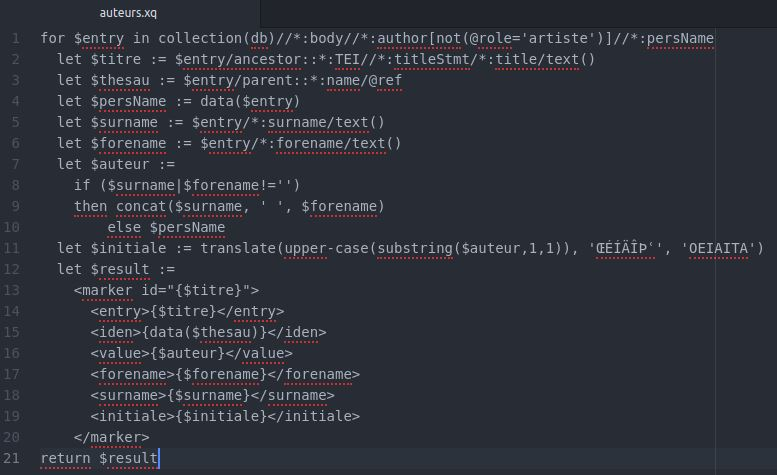
\includegraphics[width=10cm]{img/partie_1/auteurs_requete_xq.JPG}
        \caption{Fichier de requête xQuery sur les auteurs importé via BaseX.}
        \label{xq-auteurs}
    \end{figure}
    
    \begin{figure}[H]
        \centering
        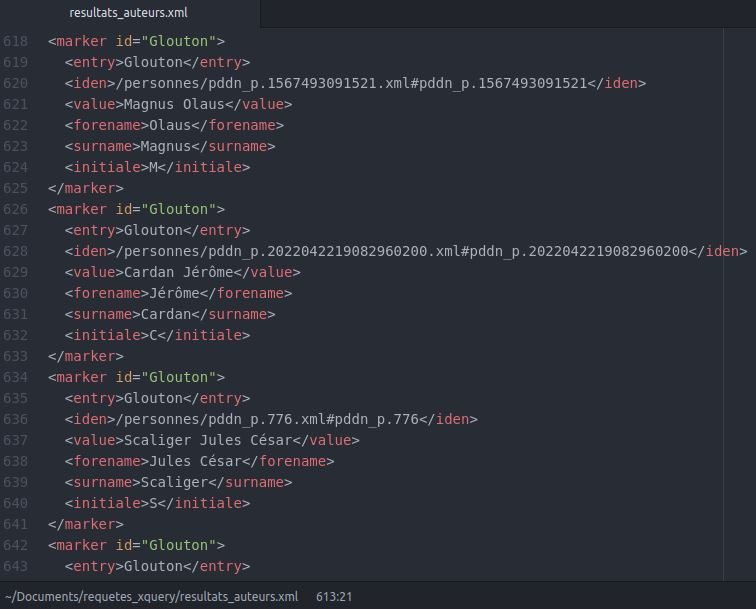
\includegraphics[width=10cm]{img/partie_1/resultats_auteurs_xml.JPG}
        \caption{Une partie des résultats de la requête xQuery sur les auteurs sous format XML.}
        \label{xml-auteurs}
    \end{figure}

    
    Le deuxième mode de fonctionnement de BaseX est en client-serveur, ce qui veut dire que l'on peut l'installer sur un serveur et l'interroger via un site Web par exemple. C'est donc avec cette brique de base que MaX a été développé.

    \begin{figure}[H]
    \centering
    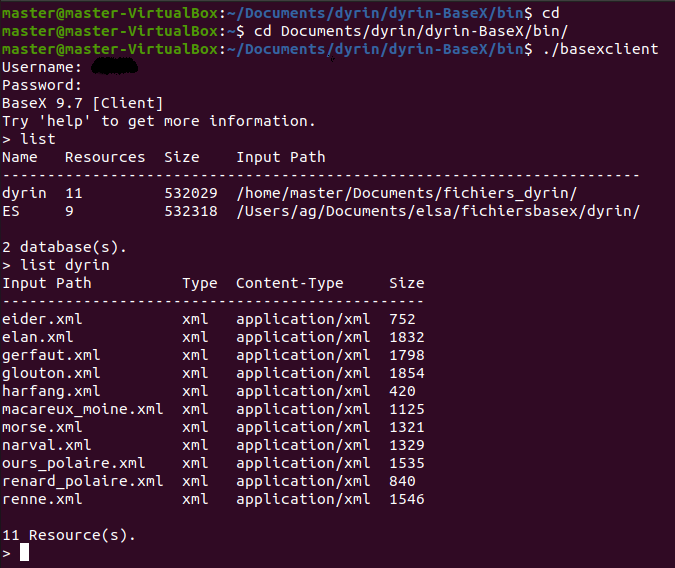
\includegraphics[width=10cm]{img/partie_1/basex_client.png}
    \caption{Capture de l'interface client de BaseX.}
    \label{bx}
\end{figure}
    
    La figure \ref{bx} ci-dessus montre l'accès à l'interface client de BaseX. C'est dans cette interface que l'on peut manipuler les fichiers de nos bases de données.
    La première étape pour pouvoir interagir avec celles-ci consiste à entrer dans le mode client-serveur de BaseX grâce à la commande \texttt{./basexclient} qui permet de lancer le script associé dans le dossier \texttt{[projet]-BaseX/bin}. L'accès est restreint par un nom utilisateur ainsi qu'un mot de passe renseigné au moment de la création de notre base de données. Par la suite, diverses possibilités s'offrent à nous. La commande \texttt{list} permet de lister toutes les bases de données créées sur BaseX. Ici elles sont au nombre de deux : Dyrin qui comporte 11 fichiers et ES qui en comporte 9. L'interface nous renseigne également sur la taille de ces bases ainsi que sur leur localisation. La commande \texttt{list [nom-de-la-base]} permet de lister les documents qui y sont présents en y dévoilant leur nom. La base de donnée est très facilement modifiable : la commande \texttt{open [nom-de-la-base]} permet d'en ouvrir l'accès afin de pouvoir y faire des modifications comme ajouter des documents (\texttt{add to [nom-de-la-base] [chemin-vers-le-fichier]} ) ou bien en retirer (\texttt{delete [nom-du-fichier]} ). La commande \texttt{close} quant à elle permet de quitter l'espace d'interaction avec la base de données.
    
    Toutes ces commandes sont intégrées dans les fonctionnalités de BaseX et n'ont pas été créées par le \acrshort{PDN} lui même. Si des modifications sont faites aux fichiers XML, il est nécessaire de les retirer de la base pour les ajouter à nouveau. Le résultat de ces changement est alors visible lors de la connection au site web.
    
    
    C'est aussi grâce aux bases de données \acrshort{XML} que le concept de travail collectif sur des sources a pu être envisagé au \acrshort{PDN}. Face à la demande et au besoin grandissant d'un travail collectif en temps-réel, la création du module collaboratif PluCo\footnote{PluCo permet d'interroger une base de données XML, d'en rapatrier des informations ou de modifier le XML. Il s'agit d'un module qui doit être intégré à un éditeur XML, il ne peut donc pas fonctionner de manière autonome. \cite{pluco}} a permis de donner un accès à distance à des données structurées à la fois aux ingénieurs et aux chercheurs. Le plugin a permis de répondre à deux grandes problématiques : la faisabilité d'un travail collectif entre ingénieurs et chercheurs ainsi que la manipulation d'arbres \acrshort{XML} présentant une arborescence très importante. En effet un problème se posait avec les plus gros fichiers \acrshort{XML} qui pouvaient mettre du temps à s'ouvrir, notamment lorsqu'y étaient ajoutées des interfaces graphiques sophistiquées comme celles produites par le \acrshort{PDN}, avec des briques comprenant beaucoup de mise en forme de branches \acrshort{XML}. \acrshort{PluCo} va permettre de pouvoir retirer un fragment de cette arborescence, juste un morceau de l'arbre, une sorte de branche de taille particulière afin de pouvoir travailler uniquement sur cette branche-là. Pour faire l'analogie, il faut imaginer un dictionnaire de 3 millions de mots, dans lequel on souhaiterait pouvoir travailler sur un terme tandis qu'un collègue travaillerait sur un autre terme : il s'agit de la même arborescence sur le serveur, cependant le travail est fait sur des fragments retirés par chacun des collaborateurs dans le cadre d'un projet.
    
    Chose importante à souligner, \acrshort{PluCo} est parfaitement intégrable à l'éditeur \acrshort{XXE}. Étant développé sous licence OpenSource, il se branche comme un plugin, comme un module d'extension et il serait donc tout à fait possible de l'adapter à d'autres éditeurs \acrshort{XML}. Sa version 2, en accès libre, est actuellement en cours de développement au \acrshort{PDN}.
    
    \section{Langage de requête : xQuery}\label{que}
    Afin de pouvoir interroger les bases de données, il est nécessaire de créer des requêtes en xQuery. Ce langage de requête est une brique technologique centrale au \acrshort{PDN}. Il s'agit d'un langage de requêtage qui permet d'interroger une base de données et d'en extraire tout ce qui correspond à des critères d'annotation \acrshort{XML} particulier. Les résultats en sortie ont une forme d'arbre XML.
    Ce langage utilise deux syntaxes particulières.
    
    La première dite syntaxe \og FLOWR \fg{} (prononcé \textit{flower}) et dont l'acronyme vient du nom des cinq principales fonctions de requête qui la compose :
        \begin{itemize}
            \item \textit{for}, pour définir le champ d'action de la requête, notamment la base de donnée explorée ;
            \item \textit{let}, pour déclarer une variable ;
            \item \textit{where}, pour déclarer des conditions (de taille, de nombre, de lieu etc.) à la requête ;
            \item \textit{order by}, pour ordonner le résultat (par ordre alphabétique, croissant, décroissant etc.) ;
            \item \textit{return}, pour indiquer la structure de sortie des données XML.
            \end{itemize}
Ce sont majoritairement des requêtes de ce style qui sont utilisées, souvent suffisantes.

La deuxième syntaxe est intitulée syntaxe XQueryX (pour \og XML Syntax for XQuery \fg), dans laquelle une requête est un document XML. De ce fait, elle est beaucoup plus verbeuse et moins lisible que la précédente et est destinée à des manipulations formelles par des programmes.


\begin{figure}[H]
    \centering
    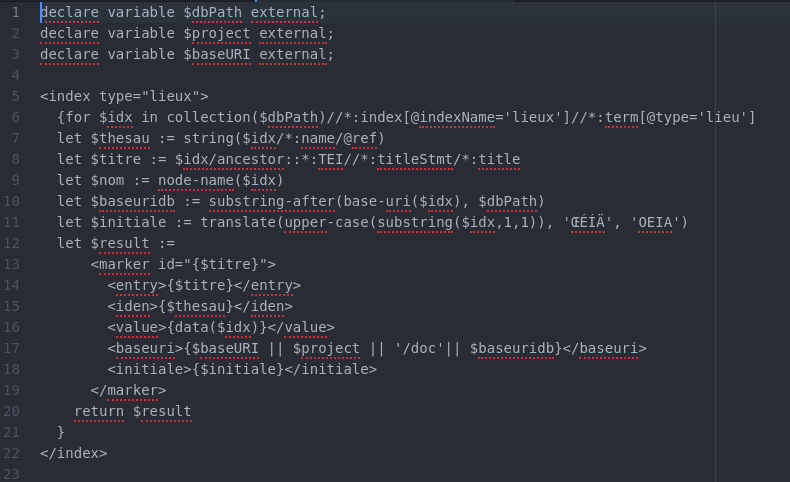
\includegraphics[width=12cm]{img/autre/xquery_exemple.png}
    \caption{Exemple de requête xQuery pour construire un index des lieux.}
    \label{xq}
\end{figure}

    L'exemple de la figure \ref{xq} ci-dessus montre une requête xQuery utilisée dans Dyrin afin de construire un index des lieux du site Web.
    
    Les différentes variables déclarées dans la requête xQuery vont permettre d'aller chercher les éléments XML dont on a besoin. Par exemple la variable \texttt{\$idx} permet de récupérer tous les éléments \texttt{<term>} de @type='lieu', eux-mêmes présents dans les balises \texttt{<index>} ayant un attribut \texttt{@indexName} égal à 'lieux'. La variable \texttt{\$titre} quant à elle va permettre de faire remonter le titre de la fiche animale en question.
    
    
    \begin{figure}[H]
  \centering
  \begin{subfigure}[b]{0.3\linewidth}
    \frame{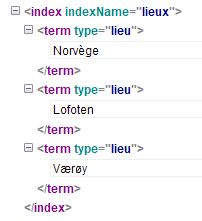
\includegraphics[width=\linewidth]{img/autre/index_lieu.JPG}}
    \caption{Exemples d'éléments XML \texttt{<term>} ciblés.}
  \end{subfigure}
  \begin{subfigure}[b]{0.4\linewidth}
    \frame{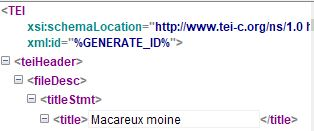
\includegraphics[width=\linewidth]{img/autre/title_fiche.JPG}}
    \caption{Élément XML \texttt{<title>} de la fiche macareux moine.}
  \end{subfigure}
\end{figure}

Le langage xQuery seul ne permet pas de mise en page HTML, mais renvoie seulement un arbre XML réorganisé avec les donnés que l'on souhaitait récupérer. C'est ce résultat de sortie qui devra être à nouveau interprété par un autre langage pour lui donner sa forme HTML finale.

    \section{L'exploitation des données: XPath, XSL}

    Ces deux langages, ce sont XPath et XML.
    
    \subsection{XPath}
    Le \acrfull{XPath} est un langage de requête permettant d'accéder à des parties de l'arborescence XML. Il rend possible un ciblage précis des éléments, tout en prenant en compte le contexte dans lequel celui-ci se trouve. Par exemple avec XPath, il est possible de chercher les éléments \texttt{<name>} présent uniquement dans des éléments \texttt{author} de la première \texttt{<div @section='source'>} du fichier XML. Les autres éléments \texttt{<name>} du document ne seront pas pris en compte. Une fois qu'une information est ciblée grâce à XPath, une transformation de l'élément sélectionné devient alors possible à l'aide du langage XSL.
    
    \subsection{XSL}
    Le langage \acrfull{XSL} est la troisième technologie utilisée au \acrshort{PDN} et permet de décrire comment doivent être transformés les documents XML. À l'intérieur même de cette technologie il en existe un très grand sous-nombre : une permet de manipuler des arbres, une autre est dédié à la production de formes PDF (il s'agit de \acrshort{XSL-FO}, longtemps montré comme un concurrent du langage de composition de documents \LaTeX)... \acrshort{XSL} est un fichier \acrshort{XML} ne contenant pas de données en particulier mais qui en respecte les principes d'écriture de base, à l'aide de balises, d'éléments et d'attributs. Il s'agit souvent de la première brique nécessaire pour travailler avec \acrshort{XML}, car, comme nous l'avons dit un peu plus haut, elle permet de passer d'un document \acrshort{XML} à un un document \acrshort{HTML}.
    
    \begin{figure}[H]
    \centering
    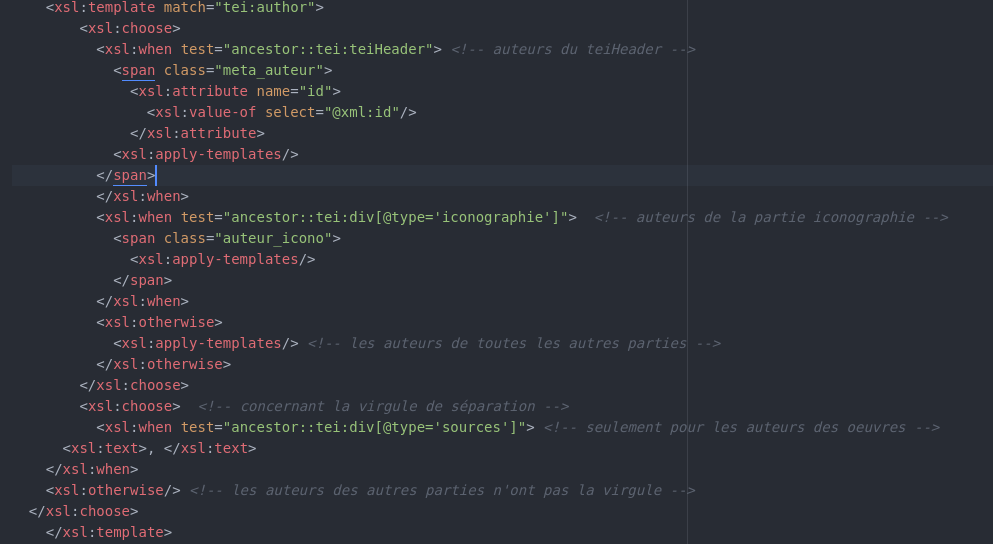
\includegraphics[width=12cm]{img/autre/exemple_xsl.png}
    \caption{Exemple de feuille \acrshort{XSL} du projet Dyrin ciblant l'élément \texttt{<author>}.}
\end{figure}

    Pour illustrer nos propos, prenons l'exemple ci-dessus de transformation \acrshort{XSL} concernant les auteurs dans Dyrin. On y \og cible\fg{} les éléments \texttt{<author>} dans le document XML et grâce au XPath on leur attribue des traitements particuliers en fonction de leur place dans l'arbre : ceux présents dans la partie du \texttt{teiHeader} du fichier XML, et uniquement eux, sont transformés en balise HTML \texttt{<span>} avec une classe \texttt{meta\_auteur} en plus d'un identifiant \texttt{id} qui prend la valeur de l'attribut \texttt{id} de l'auteur dans le XML. Ce qui correspond à cette partie de traitement :
    
    \begin{minted}{XML}
    <xsl:when test="ancestor::tei:teiHeader"> <!-- auteurs du teiHeader -->
            <span class="meta_auteur">
              <xsl:attribute name="id">
                <xsl:value-of select="@xml:id"/>
              </xsl:attribute>
            <xsl:apply-templates/>
          </span>
          </xsl:when>
    \end{minted}
    
   Lorsque les auteurs appartiennent à une partie descendant d'un noeud \texttt{div} auquel est associé l'attribut \texttt{@type} ayant pour valeur 'iconographie', ceux-ci sont entourés en HTML d'un \texttt{<span>} avec l'ajout d'une classe \texttt{auteur\_icono} comme montré ci-dessous :
    
    \begin{minted}{XML}
    <xsl:when test="ancestor::tei:div[@type='iconographie']">
    <!-- auteurs de la partie iconographie -->
            <span class="auteur_icono">
              <xsl:apply-templates/>
            </span>
          </xsl:when>
    \end{minted}
    
    Tandis que les auteurs des autres parties ne se trouvent pas à l'intérieur de balise spécifique dans le document HTML :
    
    \begin{minted}{XML}
    <xsl:otherwise>
            <xsl:apply-templates/> <!-- les auteurs de toutes les autres parties -->
          </xsl:otherwise>
    \end{minted}
    
    Et enfin, on traite différemment les auteurs en fonction de leur emplacement pour la gestion des virgules : seuls les auteurs faisant partis de la branche \texttt{<div>} de type 'sources' prennent une virgule, mais pas les autres.
    
    \begin{minted}{XML}
    <xsl:choose>  <!-- concernant la virgule de séparation -->
          <xsl:when test="ancestor::tei:div[@type='sources']">
          <!-- seulement pour les auteurs des \oe{}uvres -->
      <xsl:text>, </xsl:text>
    </xsl:when>
    <xsl:otherwise/> <!-- les auteurs des autres parties n'ont pas la virgule -->
  </xsl:choose>
    \end{minted}
    
    Dans notre rendu HTML de sortie on obtient ceci pour un auteur de la partie iconographie (visible ci-dessous en figure \ref{aut}. On remarque qu'il ne comporte pas à sa suite de virgule.
    
   \begin{figure}[H]
       \centering
       
\includegraphics[width=5cm]{img/autre/auteur_icono.png}
       \caption{Exemple d'un auteur de la partie iconographie ne comportant pas de virgule à sa suite.}
       \label{aut}
   \end{figure}

    Tandis que dans la figure \ref{auteurvir}, l'auteur est bien suivi par une virgule :
    
    \begin{figure}[H]
        \centering
        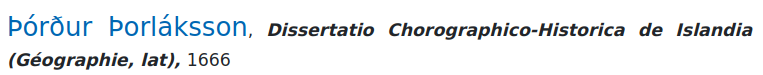
\includegraphics[width=10cm]{img/autre/auteur_virgule.png}
        \caption{Exemple d'un auteur dans la partie \oe{}uvre d'une fiche animale portant une virgule.}
        \label{auteurvir}
    \end{figure}
    
    Nous voyons donc que grâce au langage \acrshort{XSL} associé au XPath, il est tout à fait possible de traiter différemment des éléments en fonction de leur position dans l'arbre XML. Cela est rendu possible par les éléments \texttt{<xsl:choose>}, \texttt{<xsl:when>} et \texttt{<xsl:otherwise>} auxquels on vient ajouter des conditions pour indiquer les éléments précédents, concomitants ou suivants vis-à-vis de l'élément ciblé.
    
    
\section{Diffuser et accompagner}
    La version 1 de MaX, aboutissement d'une dizaine d'années de travail au \acrshort{PDN}, est sortie début avril 2022. Parallèlement à son élaboration, un gros effort de documentation\footcite{MaX} a été fait pour permettre la prise en main la plus commode possible, que ce soit pour les ingénieurs et chercheurs de l'université de Caen comme pour ceux d'autres institutions nationales. Malgré tout, il faut reconnaître que, sans la connaissance des langages \acrshort{XSL}, XPath ou xQuery, l'utilisation de MaX n'est pas évidente\footnote{Notamment lors de la création de surcharges, que nous développons plus loin en partie \ref{surcharge}}.
    
   D’où l’importance de constituer des collectifs de travail car maîtriser ces outils nécessite un temps d'apprentissage et de prise en main, cette dernière étant cependant toute relative : en effet l'utilisation de ces technologies ne requière pas une maîtrise très approfondie de l'informatique ; il n'est pas nécessaire d'être développeur pour les manipuler. L'effort à mettre en place, s'il n'est pas à minimiser, n'est pas non plus insurmontable pour la majorité des personnes. La diversité des profils représentés au \acrshort{PDN} le montre : il n'est absolument pas nécessaire de posséder un diplôme d'informatique pour comprendre de quoi il s'agit. L'exploitation élémentaire des arborescences ne nécessite pas un niveau technique ni une une formation théorique lourde, mais requiert cependant un minimum de temps pour se former. L'idée même de plate-forme impose de stabiliser des compétences et de laisser aux gens en poste le temps de se former et capitaliser dessus, tout en permettant la montée en compétence des ingénieurs sur place.
    
    
    Grâce à toutes ces briques technologiques, le \acrshort{PDN} a pu développer un outil permettant d'adapter son comportement, de prendre en compte une annotation \acrshort{XML} particulière associée à un projet, sans être obligé de re-développer l'ensemble, ni de rentrer dans des développements lourds. Telle est la spécificité de MaX : c'est sa capacité à proposer, à afficher certaine données avant même d'avoir commencé à manipuler des feuilles \acrshort{XSL} ou bien des requêtes xQuery. Mais de tout aussi bien laisser la possibilité d'ajouter une personnalisation d'un traitement particulier. À partir de ce moment alors il revient à l'ingénieur d'affiner sa requête en manipulant les langage xQuery, \acrshort{XSL} et XPath. Pour résumé, MaX a été développé pour faciliter la tâche autant aux chercheurs qu'aux ingénieurs, là où des solutions plus centralisées nécessiteraient une prise en main un peu plus délicate.
    
    
    Nous avons donc vu dans cette première partie l'importance donnée au partage entre les institutions dans la recherche en sciences humaines. Cela est rendu possible grâce à la mise en place d'un vocabulaire partagé qui se traduit par des normes techniques et des typologies communes. Tout cela a donc mené à la création de l'outil MaX, outil propice à l'innovation scientifique et technique autant pour les institutions de recherche que d'ingénierie.
    
\part{Le Moteur d'affichage XML MaX}
    
\chapter{Présentation}
MaX est un outil de production d'interfaces de lecture pour des sources \acrshort{XML} dans un environnement web. Il a été développé par le \acrfull{CERTIC} et le \acrshort{PDN}, la version 1 étant sortie début avril 2022. L'outil repose sur le système de base de données \acrshort{XML} native BaseX et sur les technologies RESTXQ\footnote{RESTXQ est une API qui facilite l'utilisation de xQuery comme langage de traitement côté serveur pour le Web. \cite{xquery}} et XSL.

Il s'agit d'un outil extensible capable de produire des interfaces de lecture pour tous les standards \acrshort{XML}. Il propose par défaut un certain nombre de modules pour la \acrshort{TEI} et l'EAD. Cet outil est l'aboutissement de plus de dix années de réflexions au \acrshort{PDN} sur l'édition de sources numériques. En effet, chaque projet développé par le \acrshort{PDN} a permis de créer des solutions technologiques que nous appellerons des \textit{briques} et qui, mises bout-à-bout, ont permis de développer MaX. Initialement développé pour les ingénieurs et chercheurs de l'université de Caen, l'outil a peu à peu été pensé comme une solution de traitement XML à vocation nationale. Pour quelles raisons et par quels moyens ? Nous étudierons pour répondre à cela son principe de fonctionnement de même que sa structure pensée pour faciliter le travail de l'éditeur ingénieur. Puis nous étudierons ce qui fait de MaX un outil pratique, à vocation universelle, poussé par l'importance croissante des pratiques FAIR du numérique.

\section{Installation}

\begin{figure}[H]
    \centering
    \frame{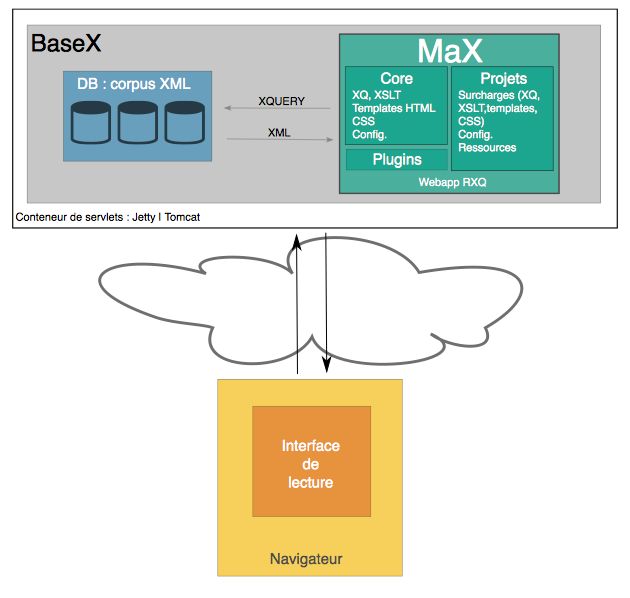
\includegraphics[width=10cm]{img/MaX/architecture.png}}
    \caption[Fonctionnement et relations de l'API MaX]{Fonctionnement et relations de l'API MaX\footnotemark.}
    \label{max}
\end{figure}
\footnotetext{\cite{MaX}}

MaX repose sur la technologie du \acrlong{SGBD} BaseX. BaseX contient des \acrfull{DB} représentées par les trois cylindres noirs dans le schéma \ref{max} ci-dessus, composées chacune de plusieurs fichiers XML dont le regroupement est qualifié de \textit{corpus}. Ces \acrshort{DB} sont modifiables via l'interface client comme expliqué dans la partie \ref{basex}. Par ailleurs, MaX est relié aux différentes éditions créées.
Plusieurs pré-requis sont donc nécessaires à l'installation de MaX :
\begin{itemize}
    \item un Système d'exploitation linux ou mac OS.
    \item Java 8+\footnote{Java est un langage de programmation qui permet de développer des applications web-serveurs.}
    \item BaseX 9.2+.
\end{itemize}

Pour chaque projet, l'utilisateur aura besoin de télécharger une application BaseX, actuellement la version 9.6\footcite{download-basex}, ainsi qu'une instance de MaX dont la dernière version est disponible sur la page GitLab\footnote{GitLab est un logiciel libre de forge, c'est-à-dire de gestion et de maintenance collaborative de textes, basé sur le logiciel de gestion Git. } du PDN\footcite{pdn-certic}.\\
À l'issu de cette procédure, la structure recommandée par la documentation étant la suivante, chaque dossier [projet] contiendra :
\begin{itemize}
    \item un dossier BaseX nommé \texttt{[projet]-BaseX}
    \item un dossier nommé \texttt{[projet]-editions} contenant toutes les éditions créées
    \item un dossier MaX nommé \texttt{[projet]-MaX}
\end{itemize}

La figure \ref{structure_dyrin} ci-dessous est un exemple de la structuration de Dyrin.

\begin{figure}[H]
    \centering
    \frame{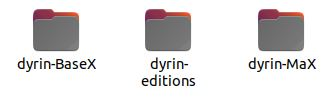
\includegraphics[width=8cm]{img/partie_2/structure_dyrin.JPG}}
    \caption{Exemple de la structure du projet Dyrin.}
    \label{structure_dyrin}
\end{figure}

Le respect de cette structure est recommandé pour pouvoir s'y retrouver dans les instructions de la documentation lors de la création d'une édition. Les dossiers seront liés les uns aux autres au moyen de \textit{liens symboliques}. Un lien symbolique est un lien créé entre deux dossiers permettant de les relier sans avoir besoin d'éditer ce même fichier/dossier plusieurs fois ou pour éviter d'avoir à déplacer des fichiers/dossiers.  Grâce au lien symbolique, si un fichier est édité, les modifications apportées apparaissent automatiquement dans tous les fichiers liés. Une illustration est donnée en guise d'exemple dans la figure \ref{lien} ci-dessous :

\begin{figure}[H]
    \centering
    \frame{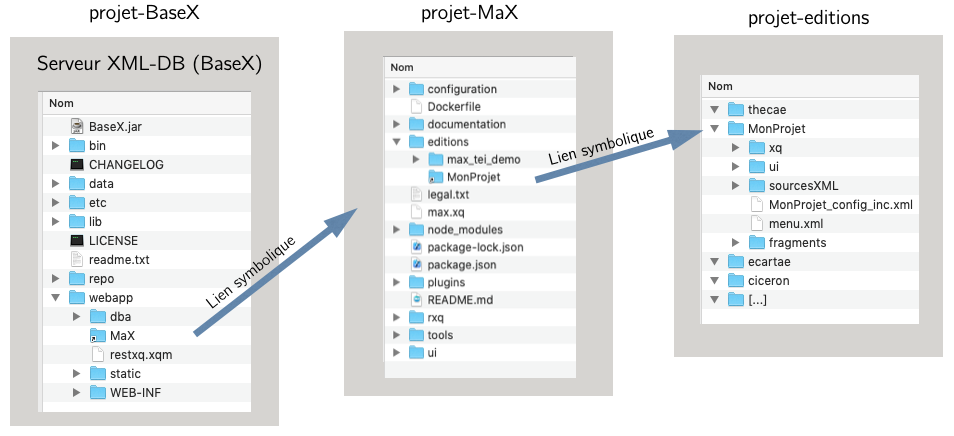
\includegraphics[width=13cm]{img/partie_2/liensSymboliques.png}}
    \caption[Représentation des différents liens symboliques présents entre chaque dossier]{Représentation des différents liens symboliques présents entre chaque dossier.\footnotemark}
    \label{lien}
\end{figure}
\footnotetext{\cite{maxdoc}}



Il faut ensuite initialiser MaX et créer les dépendances nécessaires à certaines fonctionnalités de l'outil. On utilise les termes de \og dépendances\fg{} ou de \og librairies\fg{} pour renvoyer à des logiciels externes à MaX dont il a besoin pour certaines de ses fonctionnalités. Ces dépendances sont installées grâce à la commande \texttt{./max.sh -i}. Cette commande lance l'exécution d'un script qui permet également la création de fichiers essentiels au fonctionnement de l'application comme par exemple le fichier de configuration du projet.

\section{Création d'une édition
}
Afin de pouvoir créer un site, il est nécessaire de créer tout d'abord une édition. Cette édition sera associée à BaseX. Au moment de l'installation de MaX, l'installation de deux éditions de démonstration sont proposées à l'utilisateur afin que ce dernier puisse se familiariser avec l'outil : il existe une version d'édition TEI et une autre version pour la gestion de formats EAD. Avant de créer une édition il est indispensable de lancer le serveur HTTP BaseX en se plaçant dans le dossier \texttt{[projet]/[projet]-BaseX/bin} et en lançant la commande \texttt{./basexhttp}, sinon MaX générera une erreur HTTP. En effet, au lancement du site, MaX établit des requêtes vers les sources conservées par BaseX. Si BaseX n'est pas ouvert, MaX réagit comme s'il n'existait pas de fichiers à traiter.

Il faut ensuite se placer dans le dossier \texttt{[projet]/[projet]-MaX/tools} et lancer la commande \texttt{./max.sh --d-tei} pour lancer l'édition TEI (le résultat est visible dans la figure \ref{demo-tei}) ou \texttt{./max.sh --d-ead} pour l'édition en format EAD (visible dans la figure \ref{demo-ead}).

\begin{figure}[H]
    \centering
    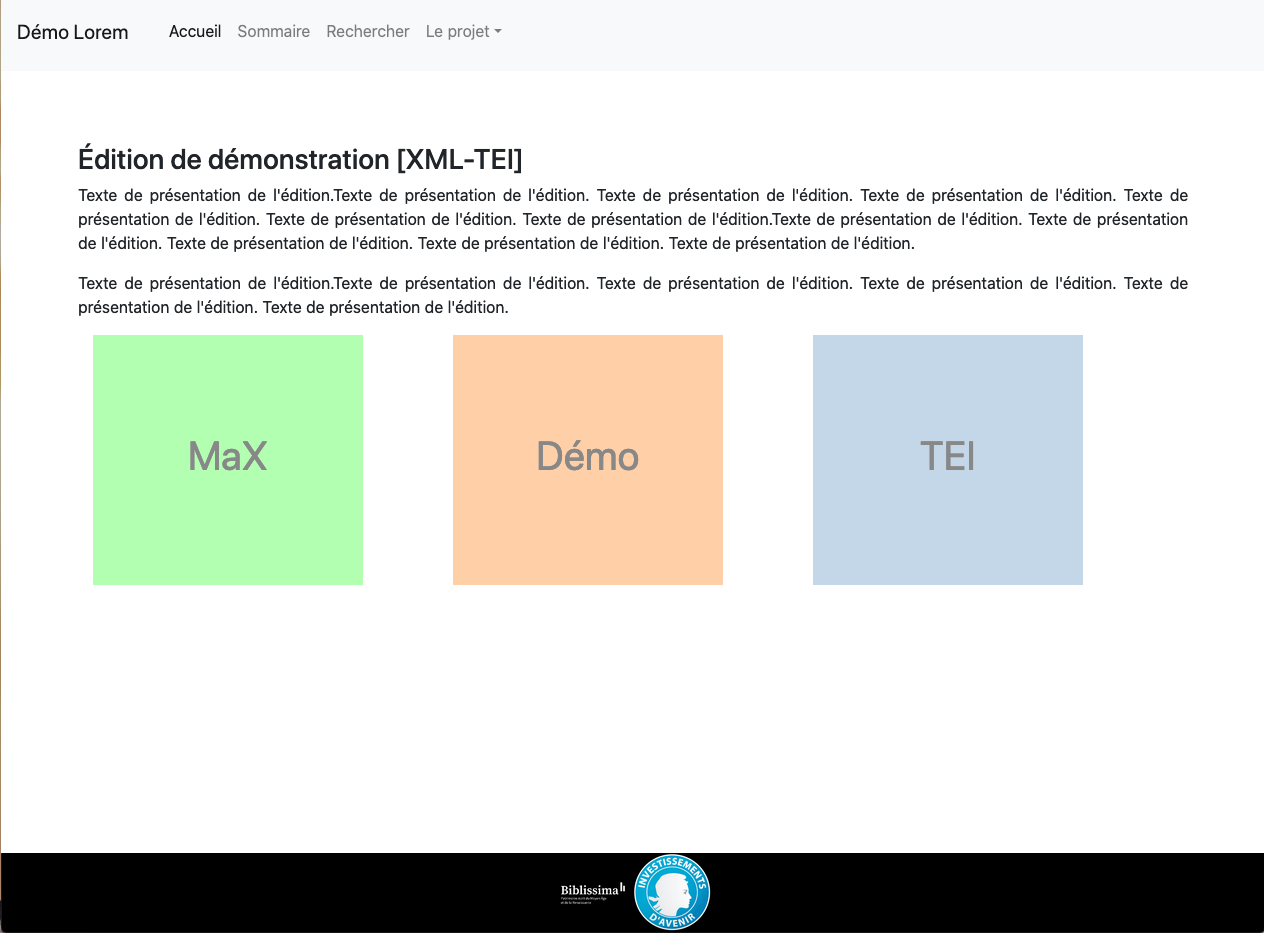
\includegraphics[width=13cm]{img/partie_2/demoTei.png}
    \caption{Page de sommaire de l'édition TEI de démonstration.}
    \label{demo-tei}
\end{figure}

\begin{figure}[H]
    \centering
    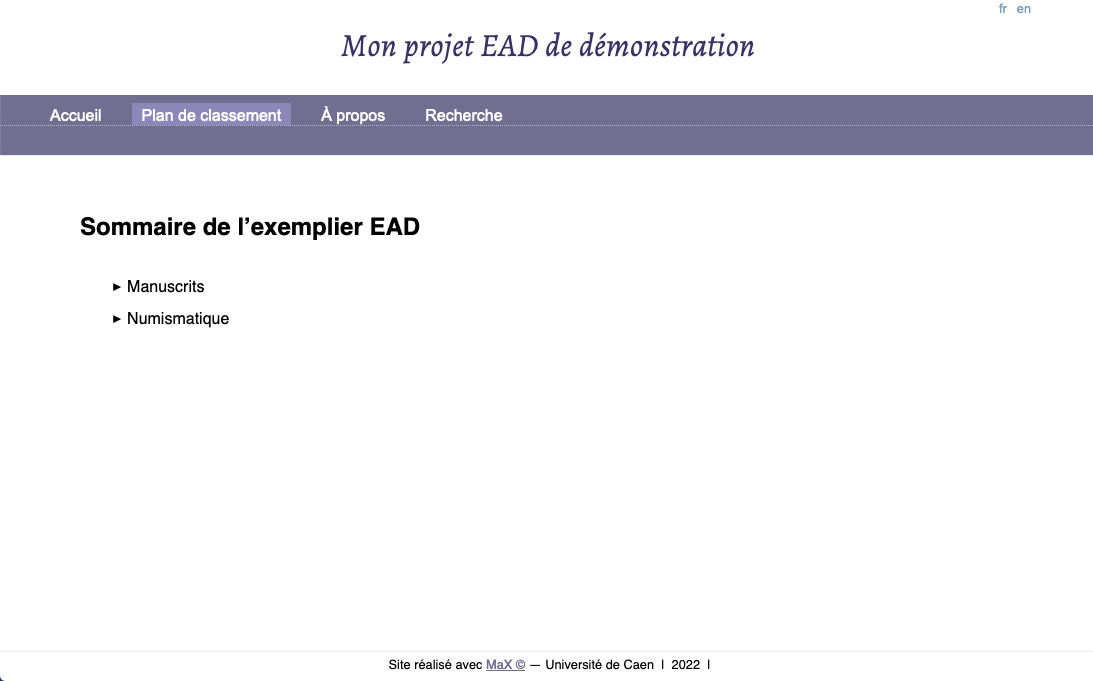
\includegraphics[width=13cm]{img/partie_2/demoead.png}
    \caption{Page de sommaire de l'édition EAD de démonstration.}
    \label{demo-ead}
\end{figure}

Cependant si l'on souhaite créer une édition avec ses propres fichiers XML, il faut suivre le processus de création d'une édition. Il faut alors se placer dans le dossier \texttt{[projet]/[projet]-MaX/tools} et lancer la commande \texttt{./max.sh -n} s'il s'agit d'une nouvelle édition et que les ports HTTP par défaut, 1984 pour le START et 8985 pour le STOP, n'ont pas été changés. Il est possible en effet de modifier ces ports s'il existe plusieurs éditions pour un seul environnement BaseX et que l'on souhaite en avoir plusieurs ouvertes en même temps. Si le port est le même pour toutes les éditions, cela ne peut être possible et déclenchera une erreur HTTP. Changer de port START et STOP doit se faire manuellement en les modifiant directement depuis le fichier caché \texttt{.basex} à la racine du dossier \texttt{[projet]-BaseX}. Si les ports on été modifiés c'est donc une autre commande qu'il faudra appeler : \texttt{./max.sh -p [numero-de-port-START] -n}.

 \begin{figure}[H]
  \centering
  \begin{subfigure}[b]{0.4\linewidth}
    \frame{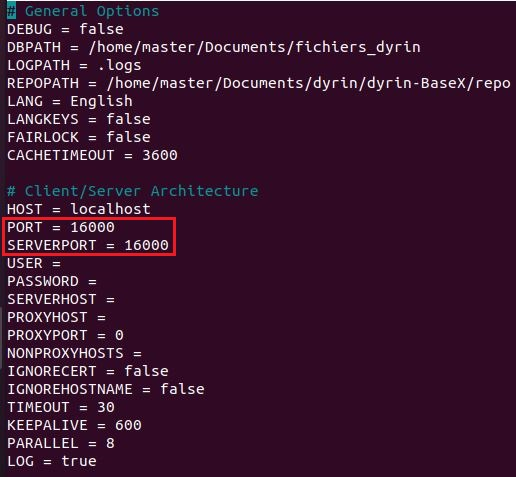
\includegraphics[width=\linewidth]{img/partie_2/port.JPG}}
  \end{subfigure}
  \begin{subfigure}[b]{0.4\linewidth}
    \frame{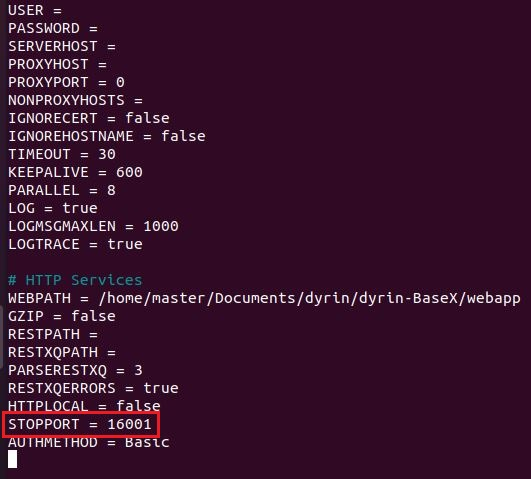
\includegraphics[width=\linewidth]{img/partie_2/port_stop.JPG}}
  \end{subfigure}
  \caption{À gauche, définition du port \textit{START} de Dyrin sur 16000 et à droite du port \textit{STOP} sur 16001.}
\end{figure}

Une fois le serveur lancé, MaX procède à la création du fichier de configuration \texttt{mon-edition\_config\_inc.xml}\label{config} à travers plusieurs questions posées à l'utilisateur:
\begin{itemize}
    \item \textit{Project ID ?} Il convient de saisir le nom du site, sans espace ni caractères spéciaux. Par exemple : dyrin
    \item \textit{XML Project type (tei, ead, ...) ?} Il faut ici saisir \textit{tei} ou \textit{ead}, selon le type de fichier du projet développé.
    \item \textit{Database path ? }Il s'agit ici de renseigner le nom de la base de données XML sans diacritique ni espace. Par exemple : dyrindb
    \item \textit{XML sources path ?} On doit alors renseigner le chemin complet vers le dossier où se trouvent les sources XML. Ce dossier ne doit contenir que des fichiers XML (aucun autre type de fichier), et uniquement les fichiers XML qui doivent être versés dans la base. Un exemple : \texttt{/home/master/Documents/fichiers\_dyrin}
    \item \textit{Please type your BaseX login/password} : cette dernière étape consiste à définir un nom d'utilisateur ainsi qu'un mot de passe qui seront demandés à l'éditeur qui souhaitera accéder à la base de données via l'outil client de BaseX.
\end{itemize}

Ces informations se retrouveront dans le fichier \textbf{[edition]\_config\_inc.xml} véritable carte d'identité de l'édition. À l'issue de cette procédure, il est désormais possible de se connecter via un navigateur en local à l'adresse suivante : \url{http://localhost:[numero-de-port]/mon-edition}. Par exemple pour Dyrin on aurait \url{http://localhost:16000/dyrin}. Il est alors possible d'accéder à son édition et de naviguer entre les différents liens présents. Chaque lien correspond à chacun des fichiers présents dans le corpus XML de BaseX.

\begin{figure}[H]
  \centering
    \frame{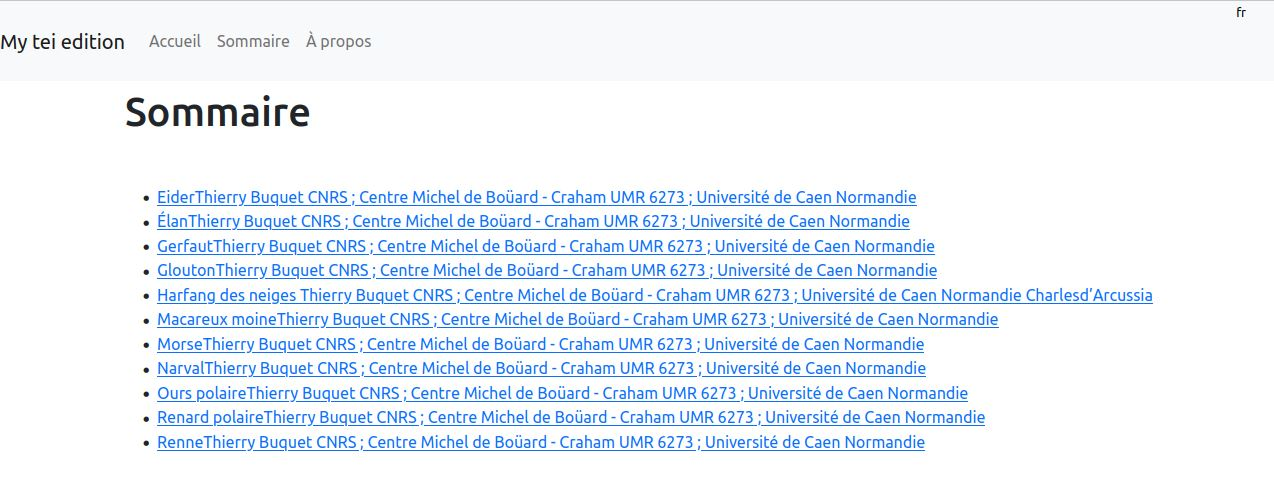
\includegraphics[width=12cm]{img/partie_2/sommaire_max.JPG}}
    \caption{Sortie \acrshort{HTML} du sommaire du projet Dyrin pris en charge par MaX.}
\end{figure}

\begin{figure}[H]
    \centering
    \frame{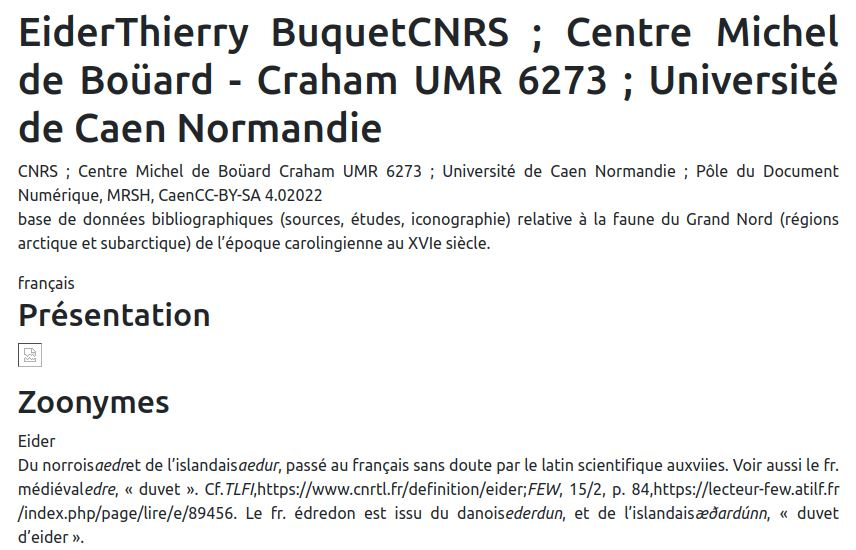
\includegraphics[width=13cm]{img/partie_2/eider_max.JPG}}
  \caption{Un exemple de sortie \acrshort{HTML} pour la fiche animale de l'eider.}
  \label{max-animal}
\end{figure}

Dans la figure \ref{max-animal} ci-dessus on remarque que certaines données apparaissent plus ou moins bien sans véritable mise en forme esthétique. Il sera par la suite possible d'y remédier grâce à des surcharges (voir la partie \ref{surcharge}) pour modifier la sortie \acrshort{HTML} de nos données. Quoi qu'il en soit, MaX fait bien ce pour quoi il a été développé : donner une première visualisation de nos sources XML sans avoir eu besoin d'éditer le moindre fichier. 


\chapter{Structure et fonctionnement}

\section{Le dossier [projet]-MaX}

Le dossier \texttt{[projet]-MaX}, un des trois piliers avec \texttt{[projet]-BaseX} et \texttt{[projet]-editions}, est en réalité le même dossier téléchargé plus tôt sur la page du \acrshort{CERTIC} mais que la structure recommandée appelle à renommer ainsi. En effet, l'application s'organise selon une arborescence très spécifique que l'on peut retrouver plus bas dans la figure \ref{arbo}.

Au sein de l'encadré rouge, à gauche, se trouve représenté le \og coeur de MaX\fg. Ce sont les dossiers et les fichiers récupérés avec l'installation de MaX. À droite, au sein de l'encadré bleu, nous avons la partie \og edition\fg. Pour joindre les deux il est nécessaire de créer un lien symbolique de l'édition dans le dossier \texttt{[projet]-edition/[edition]}, représenté au sein de la figure \ref{arbo} par une flèche allant d'un encadré à l'autre. Grâce à cela, toutes les modifications apportées dans notre édition seront automatiquement rapportées dans \texttt{[projet]-MaX} qui lui même est relié à \texttt{[projet]-BaseX}. Le dossier \texttt{[projet]-MaX} s'organise de la façon suivante :

\begin{itemize}
    \item un dossier \texttt{configuration} contenant les fichiers de configuration, d'identité du projet et des éditions créées.
    \item un dossier \texttt{documentation} qui comporte toutes les pages \acrshort{HTML} de la documentation.
    \item un dossier \texttt{editions} dans lequel on va retrouver toutes nos éditions.
    \item un dossier \texttt{plugins} qui comporte la liste des plugins importables (voir partie \ref{plugin}).
    \item un dossier \texttt{rxq} et un autre \texttt{tools} contenant les fichiers de transformation de configuration de l'édition.
    \item un dossier\label{ui} \texttt{ui} qui contient d'autres dossiers comme celui appelé \texttt{xsl} où l'on retrouve toutes les feuilles de transformation \acrshort{XSL} pour passer du XML au \acrshort{HTML}, de même que le dossier \texttt{css} responsable de la mise en forme côté client, ou bien encore le dossier \texttt{i18n} pour les versions du site en langue étrangères.
    \item le dossier contient également des fichiers comme un \texttt{readme.md} décrivant le rôle de MaX, la licence utilisée (davantage détaillée dans le fichier \texttt{legal.txt}), les pré-requis, la procédure d'installation ou bien encore les contacts des développeurs de l'application. En somme, comme tous les README, c'est une sorte de mode d'emploi.
\end{itemize}
On retrouve la même structuration du dossier \texttt{ui} au sein de ces sous-dossiers pour la configuration d'une édition particulière, c'est-à-dire dans le dossier \texttt{[projet]-editions}.


\begin{figure}[H]
    \centering
    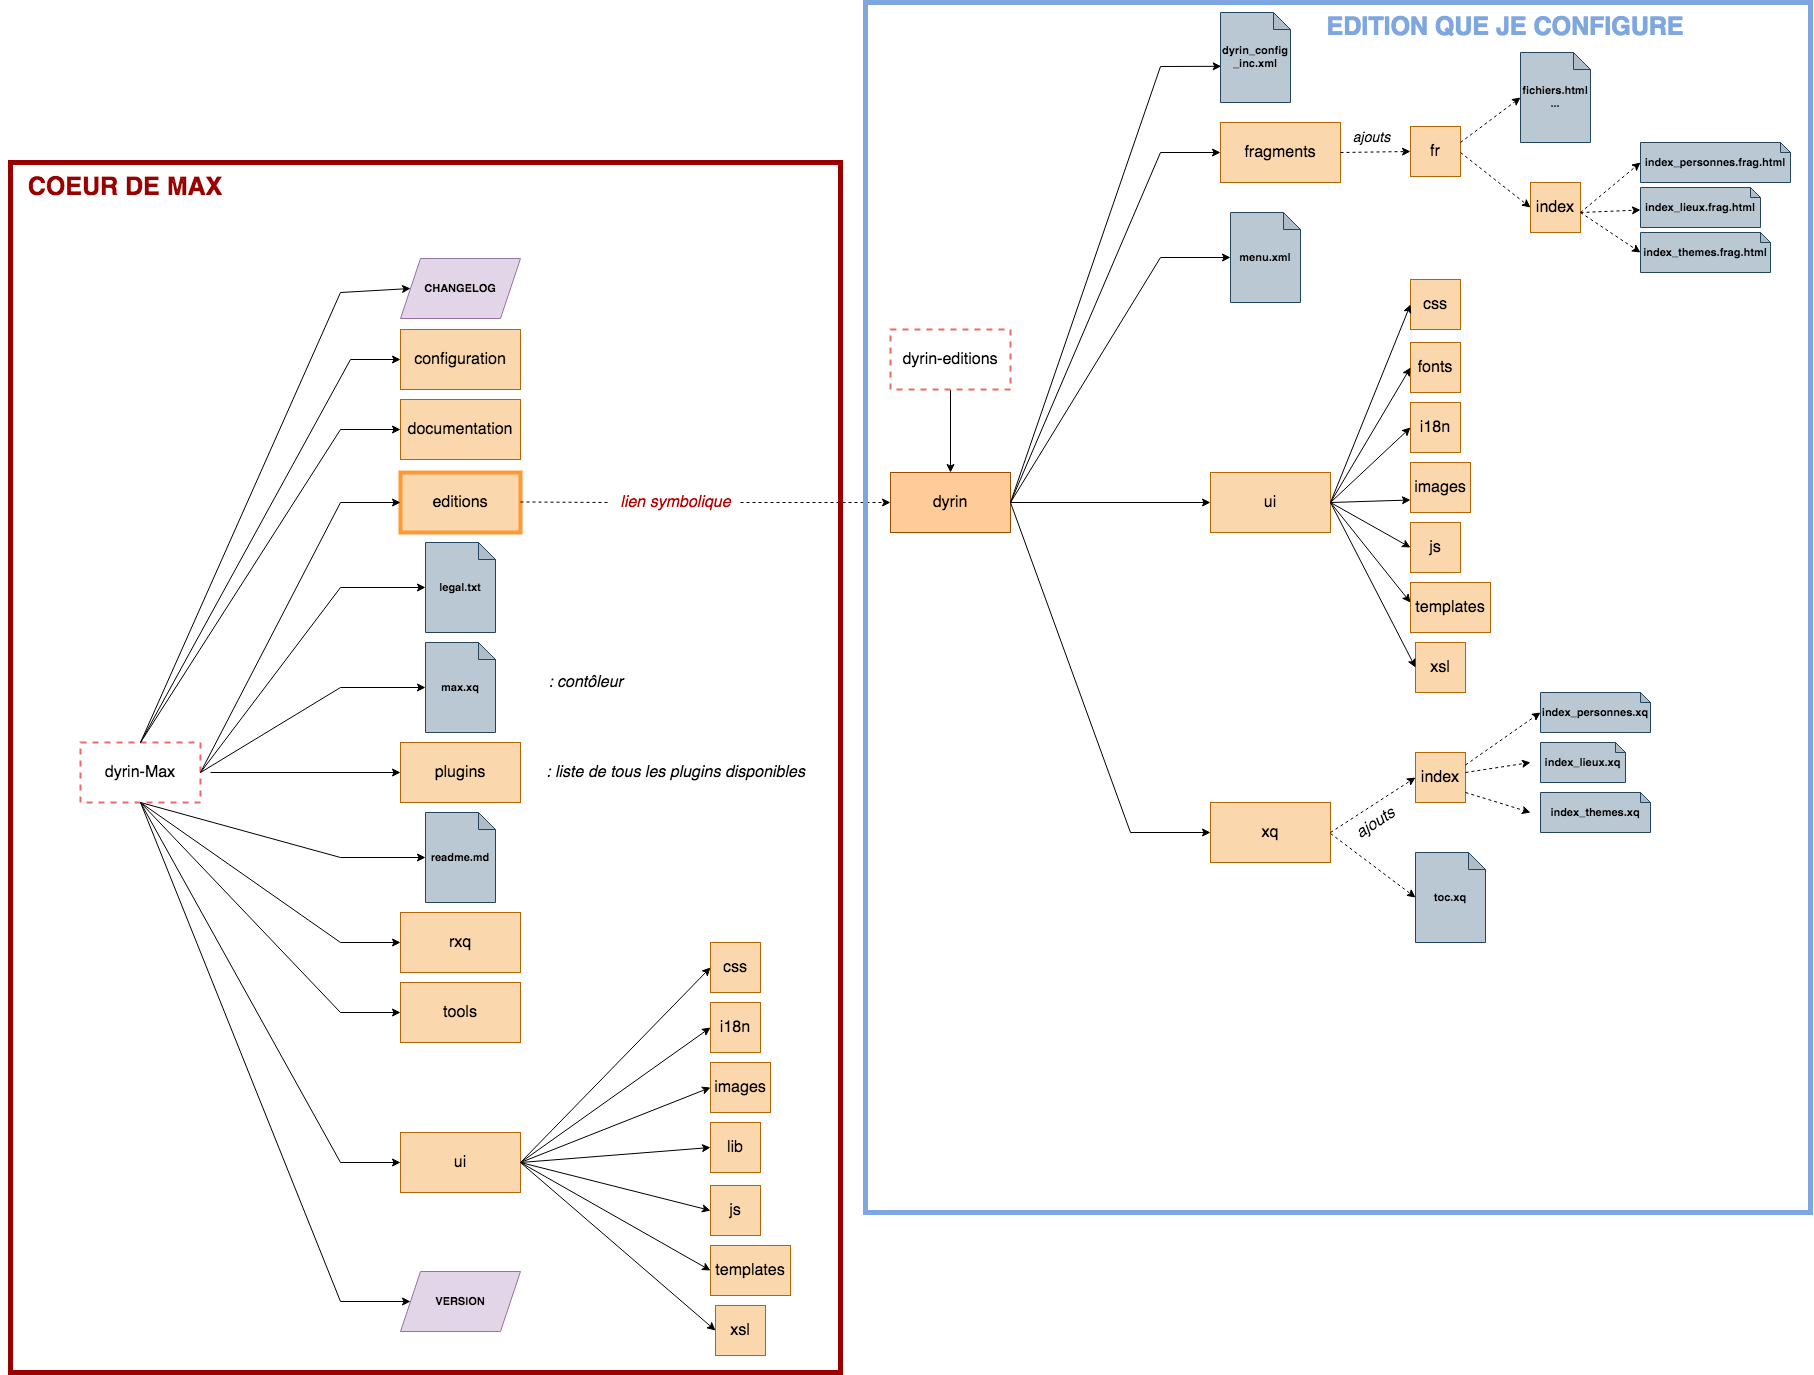
\includegraphics[width=18cm]{img/MaX/structure_MaX.png}
    \caption{Structure du c\oe{}ur de MaX et d'une édition associé (ici Dyrin).}
    \label{arbo}
\end{figure}


Le c\oe{}ur de MaX est une entité fragile et complexe : il a été développé de telle manière à ce qu'il puisse prendre en charge de manière autonome l'affichage de sources XML. Les fichiers qui le composent sont interdépendants et ne doivent pas être modifiés, au risque d'y apporter des changements irréversibles qui pourraient le rendre inopérant. Les seuls dossiers de \texttt{[projet]-MaX} dans lesquels il est possible d'apporter des modifications sont ceux intitulés \texttt{editions}, qui est en fait relié à nos éditions créées, et  \texttt{plugins}, ces fichiers n'entrant pas dans la configuration automatique de MaX.

\section{Le dossier [projet]-editions}
Ce dossier, deuxième pilier central, n'existe pas au moment de l'installation de MaX. Il s'agit en fait du dossier \texttt{editions}, constitué à l'issu de la création d'une édition, initialement présent dans \texttt{[projet]-MaX} et qui est déplacé et renommé. On vient créer par la suite le lien symbolique entre les deux afin que les modifications apportées dans \texttt{[projet]-editions} soient reportées et interprétées directement dans \texttt{[projet]-MaX}.

\begin{figure}[H]
    \centering
    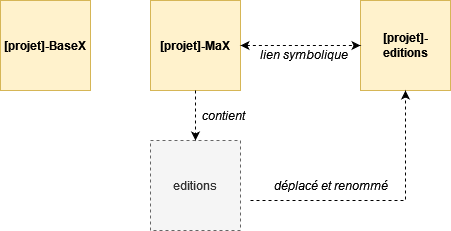
\includegraphics[width=10cm]{img/partie_2/editions.png}
    \caption{Le dossier editions déplacé et renommé devient \texttt{[projet]-editions}.}
\end{figure}

Un dossier d'édition, que l'on peut retrouver dans un état plus développé dans la figure \ref{arbo}, est composé de la manière suivante :
\begin{itemize}
    \item un dossier \texttt{fragments} qui comporte lui même un dossier \texttt{fr} contenant la page statique \acrshort{HTML} intitulée \texttt{about.frag.html}, appelée à être éditée par la suite.
    \item un dossier \texttt{ui} de même composition que décrit plus haut en \ref{ui}.
    \item un dossier \texttt{xq} vide.
    \item deux fichiers .xml indépendants : le premier intitulé \texttt{menu.xml} et qui gère l'affichage \acrshort{HTML} de la barre de navigation. Le second   \texttt{[projet]\_config\_inc.xml} qui contient les caractéristiques d'identification de l'édition (\textit{id}, \textit{dbpath}, \textit{environnement}, \textit{prettyName}) vu en \ref{config}.
\end{itemize}

Une seule instance de MaX peut accueillir plusieurs éditions. Dans le cas de notre projet Dyrin, MaX n'est relié qu'à un seul dossier d'édition. Mais par exemple, pour le projet laboratoire Norécrit\footcite{norecrit} de sources normandes, on compte 34 corpus d'édition différents !

\begin{figure}[H]
    \centering
    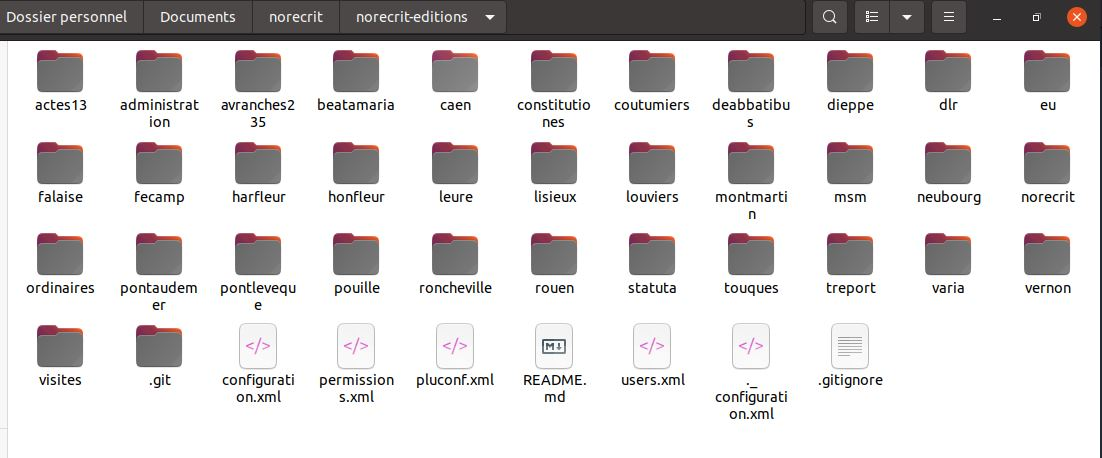
\includegraphics[width=12cm]{img/partie_2/norecrit.JPG}
    \caption{Les 34 dossiers d'édition du projet Norécrit du \acrshort{PDN}.}
\end{figure}

\section{Url et routes}
Pour la consultation d'une page d'une édition, MaX se base sur l'url interrogée. Cette url va permettre de déclencher une route à laquelle correspond un ensemble de traitements (de l'affichage d'une page \acrshort{HTML} simple, au requêtage de la base de données \acrshort{XML} pour générer une nouvelle page \acrshort{HTML} via une transformation \acrshort{XSL}). L'url contient systématiquement l'identifiant de l'édition consultée. Cet identifiant, plus d'autres paramètres optionnels, permettent de construire le document adéquat, en s'appuyant également sur le fichier de configuration de l'édition (pour les options d'affichage ou l'utilisation des plugins par exemple).

Les principales url de consultation sont les suivantes :

\begin{itemize}
    \item \url{http://[host]:[port]/[edition]/accueil.html} pour la page d'accueil d'une édition.
    \item \url{http://[host]:[port]/[edition]/sommaire.html} pour la page de sommaire d'une édition, soit une liste des documents XML consultables.
    \item \url{http://[host]:[port]/[edition]/doc/[document].html} pour la consultation d'un document d'une édition.
    \item \url{http://[host]:[port]/[edition]/[document].xml/[id].html} pour consulter un fragment (qui se base sur l'attribut XML \texttt{@xml:id}) d'une édition.
    \item \url{http://[host]:[port]/[edition]/[page].html} pour n'importe quelle page de contenu \acrshort{HTML} statique.
\end{itemize}

Au moment de la consultation de n'importe lesquel de ces url, MaX effectue un requêtage xQuery afin de récupérer les données souhaitées (liste de documents, document complet, fragment d'identité \texttt{@xml:id} etc.). Il transforme ensuite ces données en du contenu \acrshort{HTML} par application des fichiers \acrshort{XSL} présents dans \texttt{[projet]-edition} et dans \texttt{[projet]-MaX}. Il créé par la suite la page \acrshort{HTML} consultée à partir d'un \textit{template} \acrshort{HTML} de base auquel il ajoute les données transformées (blocs de navigation, menu etc.) de même que les imports \acrshort{CSS} et Javascript nécessaires. Enfin, il exécute les fonctionnalités Javascript importées via le navigateur.  
Concernant les pages \acrshort{HTML} statiques, elles se trouvent dans le dossier \texttt{[projet]-editions/[edition]/fragments/[langue-locale]} et porte chacune l'extension \texttt{.frag.html} les rendant facilement identifiables et manipulables. Le dossier \texttt{[langue-locale]} prend le nom de \texttt{fr} pour la version française du site. Les pages \acrshort{HTML} statiques telles que celles de l'accueil ou des contacts ne viennent pas avec l'installation de MaX. Il revient à l'utilisateur de créer lui même ces fichiers \acrshort{HTML}. La création de ces pages \acrshort{HTML} statiques ne nécessitent pas plus que des compétences minimes en \acrshort{HTML} et CSS.

\begin{figure}[H]
    \centering
    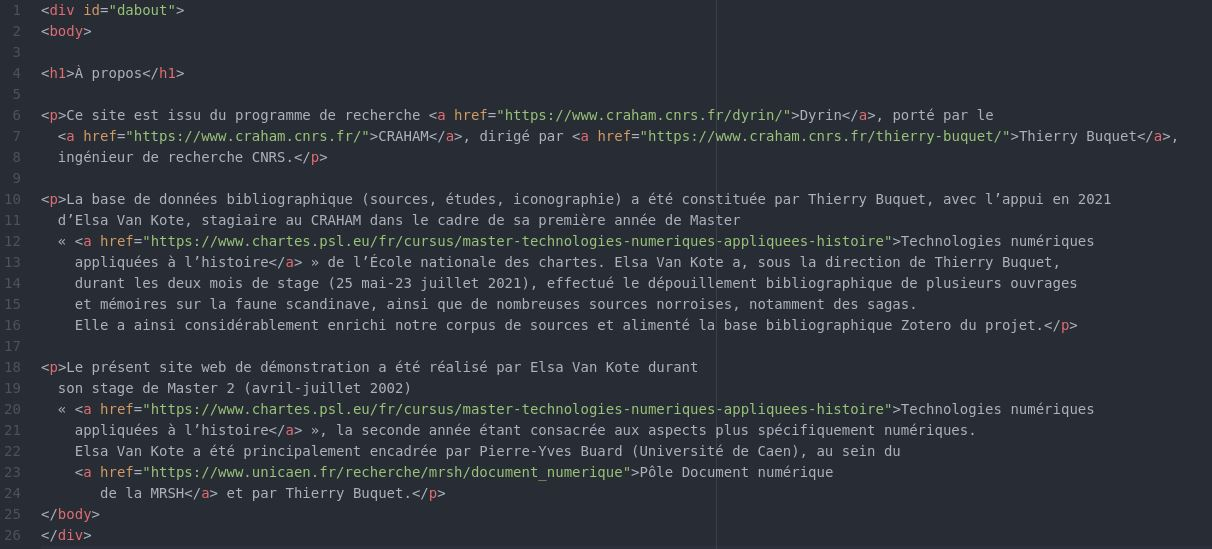
\includegraphics[width=\linewidth]{img/partie_2/a_propos_max.JPG}
    \caption{Capture du fichier \texttt{about.frag.html} du projet Dyrin.}
\end{figure}

\begin{figure}[H]
    \centering
    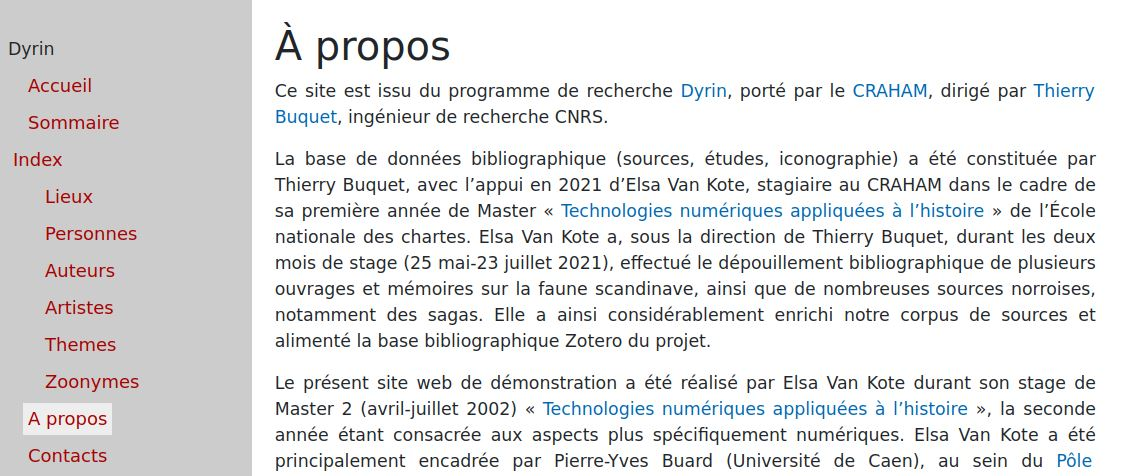
\includegraphics[width=\linewidth]{img/partie_2/a_propos_html.JPG}
    \caption{Rendu \acrshort{HTML} du fichier \texttt{about.frag.html}.}
\end{figure}


\section{Surcharges}\label{surcharge}
Le terme de \og surcharge \fg{} fait référence à l'action d'imposer un comportement nouveau à MaX venant supplanter celui proposé par défaut. Initialement, lors de la création d'un site Web, MaX va chercher en son \og coeur \fg{} les fichiers de requêtes xQuery et de transformation \acrshort{XSL} nécessaires à la création des pages \acrshort{HTML}. Cependant avant d'exécuter ces fichiers, il vérifie auparavant dans le dossier \texttt{[projet-]editions/[edition]/[ui ou xq]} pour voir s'il y trouve des fichiers \texttt{xq} et \texttt{xsl}. Si tel est le cas, il les exécute à la place de ceux en son coeur.
Ainsi pour modifier le comportement des fichiers qui se trouvent dans le c\oe{}ur de MaX, il faut créer des fichiers aux noms similaires que l'on placera dans le dossier \texttt{[projet-]editions/[edition]}. MaX en effet se repère grâce à la structure des dossiers et des noms des fichiers.  Ce sont ces fichiers de surcharge que l'on viendra éditer pour affiner nos requêtes et nos transformations.

\begin{figure}[H]
    \centering
    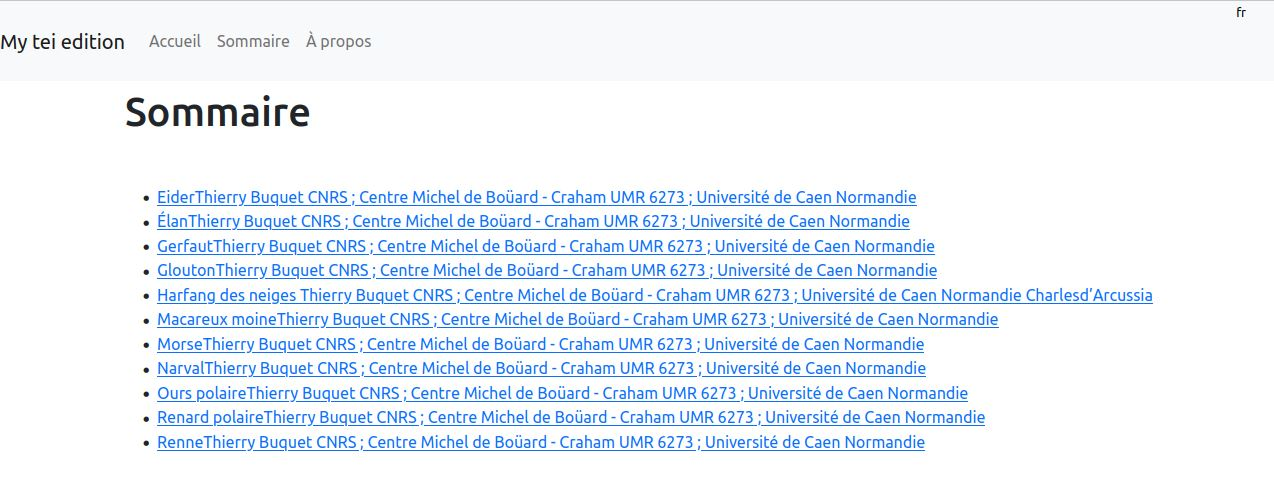
\includegraphics[width=12cm]{img/partie_2/sommaire_max.JPG}
    \caption{Sommaire pris en charge par MaX.}
\end{figure}

\begin{figure}[H]
    \centering
    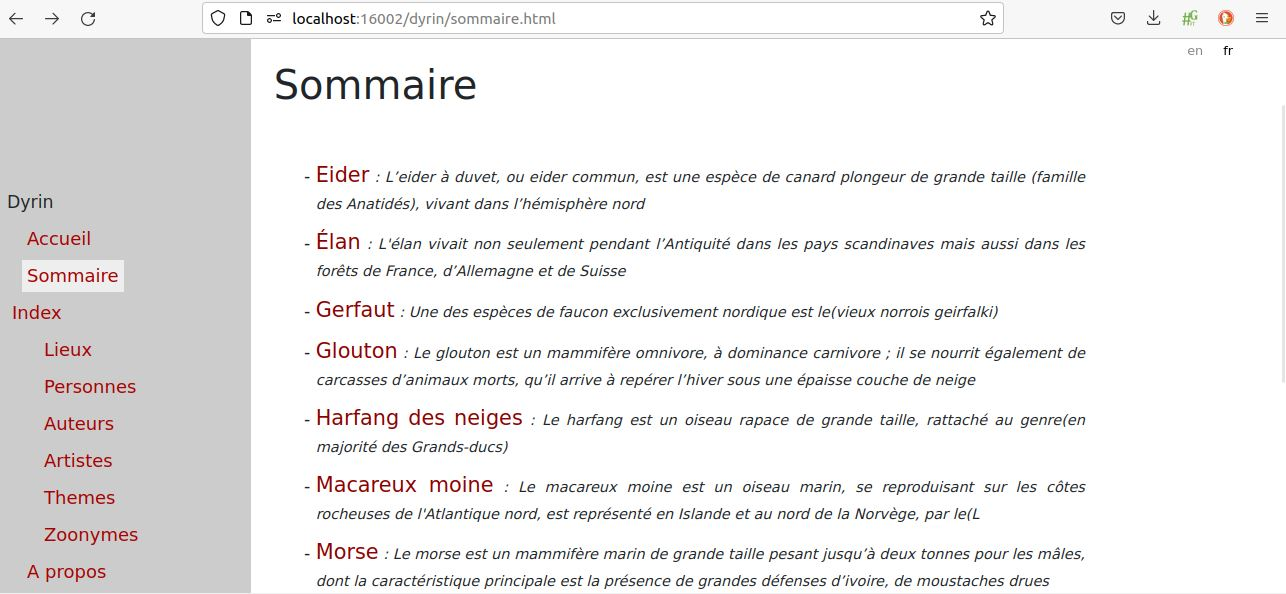
\includegraphics[width=12cm]{img/partie_2/sommaire_surcharge.JPG}
    \caption{Le même sommaire pris en charge par les surcharges \acrshort{XSL}, xQuery et \acrshort{CSS}.}
    \label{surcharge-xsl}
\end{figure}

Dans la figure \ref{surcharge-xsl} ci-dessus, on peut voir que la barre de navigation est cette fois-ci à gauche et que l'intitulé des ses sections ont été changées, notamment par l'ajout de plusieurs index. Les items du sommaire, renvoyant au fichier XML, ont également été modifiés. Par défaut, chaque item correspondait au texte qui se trouvait dans l'élément \texttt{<titleStmt>} du fichier TEI correspondant. Dans le sommaire revu par la surcharge, le nom de l'animal étudié apparaît, suivi d'un petit paragraphe de présentation. L'aspect esthétique du site (couleurs, police...) a également été revu grâce aux surcharges.


Il est possible de surcharger la quasi totalité des fichiers de MaX afin de pouvoir correspondre au maximum aux objectifs d'un projet. Ainsi la page d'accueil, le menu, le sommaire, les textes, les métadonnées \acrshort{HTML} et la mise en page sont modifiables. Cette personnalisation d'affichage des données est possible par la création du fichier le plus important de l'application, jouant un rôle de surcharge, et intitulé \texttt{text\_hook.xsl}. Ce fichier doit être placé dans le dossier \texttt{[edition]/[ui]/[xsl]}. C'est lui qui va supplanter les fichiers \texttt{tei.xsl} ou \texttt{ead.xsl} lus par défaut par MaX. Ce fichier est la feuille de transformation \acrshort{XSL} centrale qui va permettre de structurer et d'arranger les données de nos documents XML.

\begin{figure}[H]
    \centering
    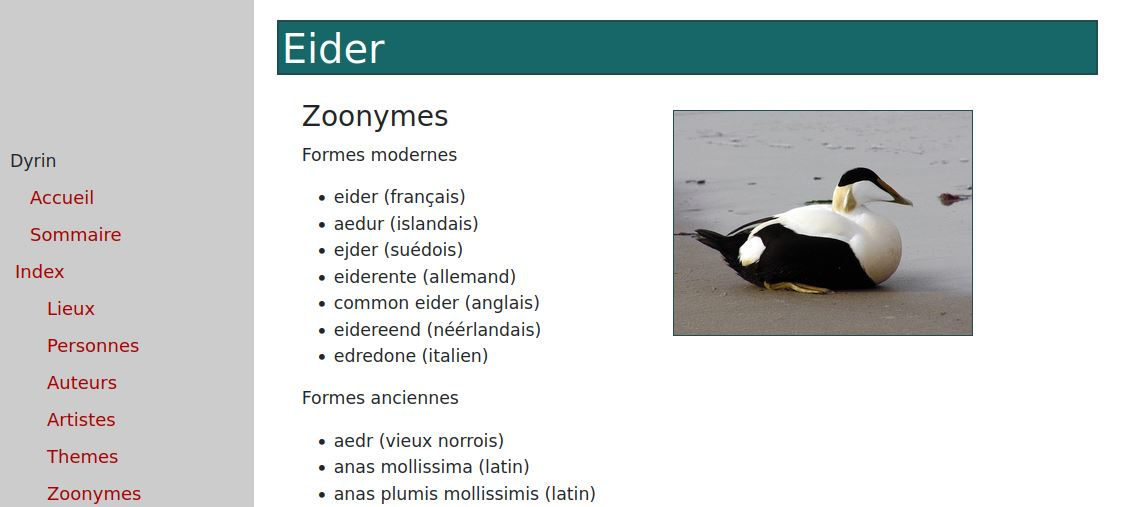
\includegraphics[width=12cm]{img/partie_2/eider_surcharge.JPG}
    \caption{La fiche eider affichant les données souhaitées grâce au fichier \texttt{text\_hook.xsl}.}
    \label{eider}
\end{figure}

On peut voir dans la figure \ref{eider} ci-dessus les zoonymes correspondant à l'eider classés en plusieurs catégories : les formes modernes et les formes anciennes. Ce choix de classement vient du porteur du projet qui a souhaité traiter ainsi les zoonymes. Ces deux catégories se retrouvent au sein du fichier XML de l'animal où elles sont indiquées par l'élément \texttt{<entry>} portant un attribut \texttt{@type} pouvant prendre la valeur de \texttt{moderne} ou bien \texttt{ancienne}. La feuille de transformation \texttt{text\_hook.xsl} va venir sélectionner ces éléments et les trier en fonction de cet attribut \texttt{@type}.

\begin{figure}[H]
    \centering
    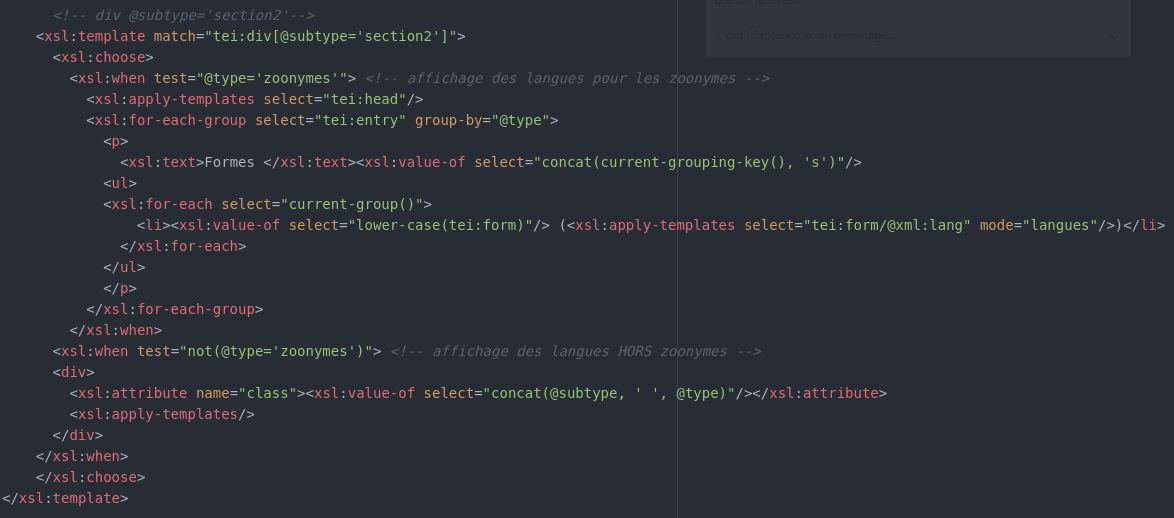
\includegraphics[width=\linewidth]{img/partie_2/zoonymes.JPG}
    \caption{Traitement de la structure des zoonymes par la feuille de transformation \texttt{text\_hook.xsl} pour la sortie \acrshort{HTML}.}
    \label{zoonymes}
\end{figure}

Dans l'extrait de code ci-dessus en \ref{zoonymes}, on peut voir que lorsque l'élément TEI \texttt{<div>} dont l'attribut \texttt{@subtype} est de valeur 'section2', on lui attribue une transformation. Pour cela on teste si cet élément possède en plus un attribut \texttt{@type} de valeur égale à 'zoonymes'. Si c'est bien le cas, on inscrit la valeur de l'élément TEI \texttt{<head>} suivie ensuite d'un tri en groupe grâce à la fonction \acrshort{XSL} \texttt{xsl:for-each-group} sur la valeur de l'attribut \texttt{@type} (\og ancienne\fg{} ou \og moderne\fg). Le résultat est inséré dans une balise \acrshort{HTML} \texttt{<p>} dans laquelle on insère une chaîne de caractères \texttt{Forme} à laquelle on ajoute la valeur de l'attribut \texttt{@type}. En somme, si la valeur est égale à \texttt{moderne} on obtient \texttt{Formes modernes}, et si elle est égale à \texttt{ancienne} on obtient \texttt{Formes anciennes}. À l'intérieur de ces groupes on trouve sous forme de liste d'éléments \acrshort{HTML} \texttt{<li>} les termes des zoonymes en questions. On trouve à la suite, entre parenthèses, la langue correspondante à ce zoonyme. L'affichage de la langue se fait grâce à la récupération de la donnée présente dans le \texttt{@xml:lang} de l'élément \texttt{<form>} du document TEI. C'est la règle : \texttt{<xsl:apply-templates select="tei:form/@xml:lang" mode:"langues"/>} qui permet cela. L'expression \texttt{@mode="langues"} que l'on retrouve dans cette règle permet d'appliquer à cette transformation une règle précédemment déclarée concernant toutes les langues du document. Pour terminer, si l'élément TEI \texttt{<div>} n'a pas d'attribut \texttt{@type} de valeur égale à 'zoonymes', la règle précédemment décrite ne s'appliquera pas.


Réaliser des surcharges requiert obligatoirement des connaissances ainsi que des compétences en technologies xQuery, \acrshort{XSL}, \acrshort{HTML} et CSS. Ces compétences sont apportées par les ingénieurs. Afin que les objectifs scientifiques du projet soient bien remplis à cette étape, il est important de concevoir entre chercheurs et ingénieurs une feuille de route précise sur ces objectifs et sur la manière dont ceux-ci vont être atteints.
Une des conséquences de cette dépendance du chercheur envers l'ingénieur est leur sollicitation permanente pour effectuer des modifications techniques. Or plus le nombre de projets sera important plus ces sollicitations seront nombreuses, tandis que les équipes d'ingénieurs ne peuvent s'étendre indéfiniment.


Dans l'optique de pouvoir se libérer du temps de recherche, le \acrshort{PDN} a développé pour MaX des \textit{plugins} permettant de répondre à des créations techniques similaires entre plusieurs projets.

\section{Plugins}\label{plugin}

Un \textit{plugin} (dans le contexte de MaX), également appelé module, est une brique logicielle proposant une fonctionnalité supplémentaire au noyau de l'application MaX. C'est avec ces plugins que sont possibles par exemple l'affichage des apparats critiques dans les sources, la gestion d'index ou bien encore la visualisation d'images. 

L'ensemble des plugins proposés, au nombre de 18, sont stockés dans le dossier \texttt{[projet]-MaX/plugins}. Pour les activer il suffit de se placer dans le dossier \texttt{tools} puis de lancer le script \texttt{max.sh} qui permet l'activation/désactivation de ces plugins. Afin de savoir quel plugin est activé ou non sur l'édition en cours, il est nécessaire de faire apparaître leur liste dans le terminal via la commande \texttt{./max.sh --list-plugins}. 


\begin{figure}[H]
    \centering
    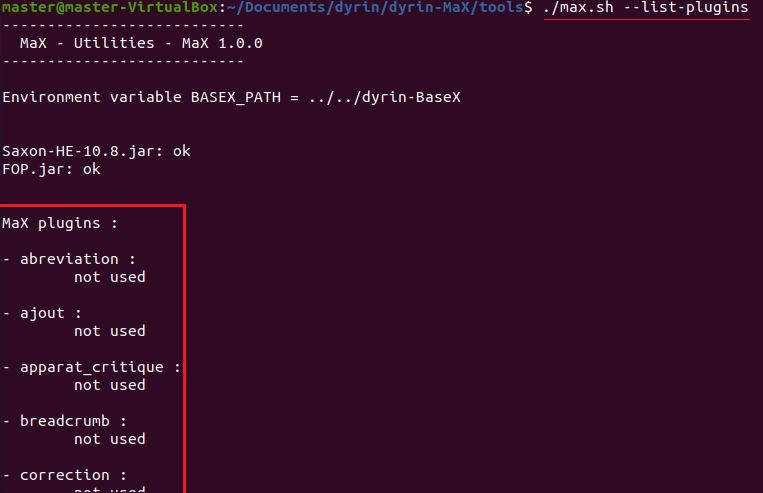
\includegraphics[width=12cm]{img/partie_2/plugins.JPG}
    \caption{Soulignée en rouge, la commande de liste des plugins. En bas à gauche, des plugins non activés encadrés en rouge.}
\end{figure}

Ces modules sont désactivés par défaut, comme l'indique la formule \textit{not used}. Mais ils peuvent être activés à tout moment grâce à la commande \texttt{./max.sh --enable-plugin [plugin\_name] [mon-edition]}. Cette commande va permettre de supprimer un fichier\textit{ .gitignore} présent dans le plugin et va également inscrire son identité dans le fichier d'identité \texttt{[projet]\_config\_inc]} en ajoutant une ligne \texttt{<plugin name="[nom-du-plugin]"/>}. Lors de la consultation d'un fragment, MaX exécute l'ensemble des xQuery des plugins actifs respectant la convention de nommage : \texttt{plugins/[nom-du-plugin]/[nom-du-plugin].xq}. 

\begin{figure}[H]
    \centering
    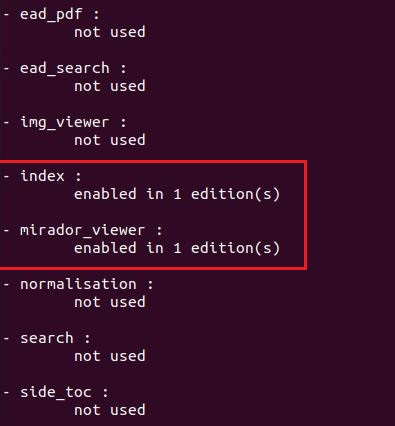
\includegraphics[width=8cm]{img/partie_2/plugins_actifs.JPG}
    \caption{Dans le cadre rouge, deux plugins actifs pour l'édition Dyrin : celui de gestion des index et celui d'affichage d'images \acrshort{IIIF}.}
\end{figure}

Certains plugins ont des dépendances vers des bibliothèques Javascript (par exemple le plugin \textit{img\_viewer} requiert l'utilisation d'OpenSeadragon\footnote{OpenSeadragon est un logiciel OpenSource de visualisation d'images : \cite{openseadragon}}) permettant par exemple l'affichage de fenêtres pop-up côté client. Ces dépendances sont appelées au moment de la structuration de la page \acrshort{HTML}, comme on peut voir dans l'exemple ci-dessous:

\begin{figure}[H]
    \centering
    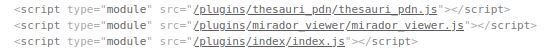
\includegraphics[width=13cm]{img/partie_2/modules_html.JPG}
    \caption{Appel des scripts Javascript des trois modules activés de l'édition Dyrin.}
\end{figure}

Ces bibliothèques sont incluses dans chacun des plugins.
À chaque plugin est associé une documentation en markdown\footnote{Le markdown est un langage de balisage créé dans le but d'offrir une syntaxe facile à lire et à écrire. \cite{markdown}} détaillant les fichiers contenus par ledit plugin.
À n'importe quel stade du travail éditorial les plugins activés peuvent être désactivés de nouveau avec la commande \texttt{./max.sh --disable-plugin [plugin\_name] [mon-edition]}.

Chacun de ces plugins permet d'insérer dans le projet une fonctionnalité supplémentaire : le plugin \texttt{thesauris\_pdn} permet de créer des liens entre les documents et des fiches d'autorité. Celui intitulé \texttt{mirador\_viewer} permet d'intégrer dans les documents des visualisations d'images et textes en haute qualité. Le dernier plugin, \texttt{index} quant à lui permet de créer des pages d'index.

Ces plugins, que nous détaillerons bien plus en détail en partie \ref{plugin}, ont été imaginés et développés par le \acrshort{PDN} au fur et à mesure des projets traités. Pour citer quelques exemples, le module \textit{apparat-critique} a été développé pour le projet Malaterra\footnote{Le projet Geoffroi  Malaterra vise à l'édition critique avec traduction française et commentaire (historique, philologique et littéraire) de l' Histoire du Grand Comte Roger et de son frère Robert Guiscard.} puis réutilisé pour Norécrit. Les modules d'\textit{abbréviation}, \textit{ajout} et \textit{correction} ont été élaborés à l'issu de la création de l'environnement inventaire ancien du projet Thecae\footnote{Thecae est une collection d'inventaires de livres médiévaux et modernes, du \textsc{viii}\ieme{} au \textsc{xviii}\ieme{} siècle, tant en caractères latins qu'en caractères grecs. Elle a été préparée par des décennies de recherche à l'IRHT et a été prévue dans le programme Biblissima avec la participation du \acrshort{CRAHAM} et de la \acrshort{MRSH} de Caen. La France se dote ainsi des premiers répertoires électroniques de sources et du premier corpus électronique d'inventaires anciens de livres (en XML-TEI), permettant d'étudier la transmission des textes sur un temps long et de façon totalement transversale. Pour plus d'information sur le projet, consulter l'adresse suivante : \url{https://www.unicaen.fr/puc/sources/thecae}\label{thecae}}. Le projet des \acrshort{BVMSM} quant à lui a permis au \acrshort{PDN} de mettre au point deux plugins de visualisation d'images: \textit{img\_viewer} pour les images classiques et \textit{mirador\_viewer} pour les définitions en format \acrshort{IIIF}\footnote{L'International Image Interoperability Framework (IIIF) désigne à la fois une communauté et un ensemble de spécifications techniques dont l'objectif est de définir un cadre d'interopérabilité pour la diffusion et l'échange d'images haute résolution sur le Web. \cite{iiif-intro}}.




\chapter{Principes FAIR et questions de maintenance}
Au sein de cette sous-partie, nous analyserons MaX sous l'angle des protocoles d'échange FAIR et essaierons de comprendre ce qui fait de MaX un outil interopérable.

\section{Suivre les principes FAIR}
Comme nous l'avons vu plus haut, MaX repose sur des standards bien implantés dans la communauté scientifique. Les langages XML-TEI et XML-EAD en sont des exemples, rendant interropérables les données numériques. L'utilisation de standards de structure facilite grandement leur réapropriation par d'autres institutions partageant les mêmes codes et outils,  quelque soit le domaine de recherche (la figure \ref{echange} plus bas illustre ces propos). Cette interopérabilité vise à permettre d'échanger et de croiser des types et formats de données très divers ; c'est l'un des principes et critères des pratiques FAIR (que représente la figure \ref{echange} ci-dessous).


\begin{figure}[H]
    \centering
    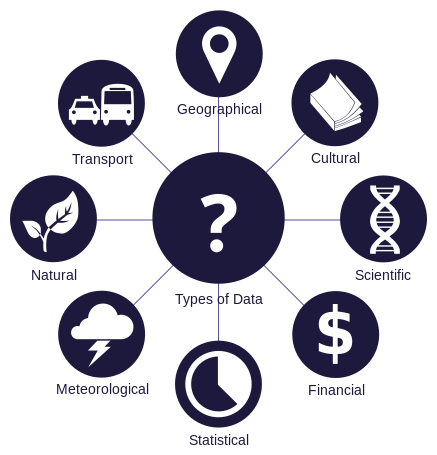
\includegraphics[width=8cm]{img/partie_2/Data_types.png}
    \caption{Les pratiques FAIR permettent de rendre interropérables des données de domaines scientifiques très différents.}
    \label{echange}
\end{figure}

\begin{quote}
    Les principes FAIR (Findable, Accessible, Interoperable, Reusable) décrivent comment les données doivent être organisées pour être plus facilement accessibles, comprises, échangeables et réutilisables. On en parle surtout pour les données de recherche mais ces principes concernent toute ressource numérique disponible en accès ouvert relative à une activité scientifique\footcite{FAIR}.
\end{quote}

Ce principe de \textit{fair data}, dont l'acronyme fait notamment référence au concept d'équité, est apparu en 2016 après la publication d'un rapport d'une communauté internationale\footcite{wilkinson_fair_2016} composée de chercheurs, de bibliothécaires, d'archivistes ou bien encore d'éditeurs, dans le journal scientifique \textit{Scientific data}\footnote{Scientific Data est une revue en libre accès évaluée par des pairs pour la description d'ensembles de données et de recherches et qui se donne pour mission de faire progresser le partage et la réutilisation des données de recherche : \cite{scientific-data}} de la revue \textit{Nature}\footnote{Nature est une revue internationale hebdomadaire publiant les recherches évaluées par des pairs dans tous les domaines de la science et de la technologie : \cite{nature}}. Cette publication décrivait les initiatives à déployer pour faire appliquer ces pratiques FAIR dans tous les domaines numériques.
Cette idée de données faciles à trouver, accessibles, interropérables et réutilisables implique un comportement pro-actif et juste de la part de leur producteur lequel, par des choix conscients, cherche à rendre ses données plus accessibles à tous sur internet, dans une logique de partage des savoirs. De nos jours, avec le recours croissant à l'intelligence artificielle, ces puits de données publiques sont un enjeu de plus en plus grand. Une donnée d'excellente qualité mais mal référencée ne pourra pas être extraite de manière évidente, tout comme une donnée facilement trouvable mais non interropérable. C'est là toute la complexité des principes FAIR : leur efficacité est optimale uniquement si toutes les cases sont remplies, et une seule règle manquante peut mettre en péril l'objectif de toutes les autres. Ces données doivent donc être facilement manipulables non seulement par l'humain mais également par la machine qui joue ici un rôle de moissonneuse dans la récolte et l'extraction d'un genre de donnée particulière. Le rôle des machines est d'autant plus important que la quantité et la complexité des données disponibles sur le web croissent de manière exponentielle.


Bien que MaX ait été initialement créé pour une utilisation limitée à l'université de Caen, l'outil a pu être diffusé en-dehors en partie grâce à des choix de développement alignées sur les pratiques FAIR.
MaX est un outil libre développé en OpenSource dont les fichiers de développement sont accessibles de manière totalement libre et gratuite. On peut le trouver sur Internet depuis n'importe quel navigateur et depuis n'importe quel moteur de recherche.
Si nous faisons l'expérience d'essayer de trouver l'outil MaX avec différents navigateurs, voici les résultats obtenus :

\begin{table}[H]
\centering
\begin{tabular}{|>{\columncolor{lightgray}}c|>{\columncolor{red}}c|>{\columncolor{red}}c|c|}
\hline
Navigateur|Recherche & \cellcolor{lightgray}max caen & \cellcolor{lightgray}MaX caen & \cellcolor{lightgray}max université caen \\
\hline
Firefox & adresse coiffeur & adresse coiffeur & \cellcolor{red}université de caen \\
\hline
Chrome & adresse coiffeur & adresse coiffeur & \cellcolor{green}outil MaX \\
\hline
Edge & adresse coiffeur & adresse coiffeur & \cellcolor{red}université de caen \\
\hline
\end{tabular}
\caption{Tableau comparatif des différents moteurs de recherche.}
\label{tableau}
\end{table}

\begin{table}[H]
\centering
\begin{tabular}{|>{\columncolor{lightgray}}c|>{\columncolor{green}}c|>{\columncolor{green}}c|>{\columncolor{orange}}c|}
\hline
Navigateur|Recherche & \cellcolor{lightgray}max unicaen & \cellcolor{lightgray}max pdn & \cellcolor{lightgray}pdn xml caen \\
\hline
Firefox & MRSH + documentation & documentation & acceuil PDN \\
\hline
Chrome & outil MaX & outil MaX & acceuil MRSH-PDN \\
\hline
Edge & MRSH + documentation & documentation & acceuil PDN \\
\hline
\end{tabular}
\caption{Tableau comparatif des différents moteurs de recherche.}
\label{seo}
\end{table}

Dans les deux tableaux ci-dessus \ref{tableau} et \ref{seo} le navigateur Firefox est utilisé avec le moteur de recherche duckduckgo. Chrome fonctionne avec Google tandis qu'Edge utilise le moteur Bing de Microsoft. On remarque que pour une même recherche (\og \textit{max caen}\fg, \og \textit{MaX caen}\fg) les résultats sont les mêmes : ils ne répondent pas à la demande initiale et sont donc marqués de rouge. Avec la recherche \og\textit{max université caen}\fg, seul Chrome parvient à rediriger vers MaX. Les deux autres navigateurs renvoient vers le site de l'université de Caen que nous considérons comme une réponse trop large. Avec les recherches \og \textit{max unicaen}\fg{} et \og \textit{max pdn}\fg{} les trois moteurs parviennent à répondre à notre demande en donnant le lien direct vers MaX via le site de la \acrshort{MRSH}, la documentation ou bien la page du \acrshort{CERTIC}. Dans le cas de la dernière recherche, \og \textit{pdn xml caen}\fg, on trouve comme réponses les pages d'accueil du \acrshort{PDN} et celle de la \acrshort{MRSH}, ce qui est acceptable, mais non totalement satisfaisant. En conclusion, nous pouvons dire que peu importe le navigateur ou bien le moteur de recherche utilisé, la mention seule de MaX ne suffit pas pour trouver l'outil. D'une part notamment car Max étant un prénom courant, cela émet beaucoup de bruit dans les résultats, comme nous pouvons le voir avec les retours concernant le salon de coiffure. D'autre part, peut-être serait-il intéressant d'accentuer l'efficacité de la recherche en lui attribuant des mots clefs comme \og édition numérique\fg{} ou bien \og XML\fg, \og TEI\fg{} ou \og EAD\fg. 

Cependant, malgré les efforts d'une meilleure indexation, chaque moteur de recherche a des algorithmes si différents qu'il est impossible de prédire une liste de résultat. Ce résultat sera de toute manière personnalisé pour chaque machine en fonction de l'historique et des préférences de l'internaute.

La première étape pour pouvoir réutiliser les données est qu'elles soient faciles à trouver que ce soit pour l'homme ou la machine. Au moment de la création d'une édition, MaX élabore des métadonnées \acrshort{HTML} pour le site Web créé. Ces métadonnées sont prises en charge par le c\oe{}ur de MaX, grâce à un fichier \texttt{html.xqm} que l'on peut voir dans la figure infra \ref{metadata}.


\begin{figure}[H]
    \centering
    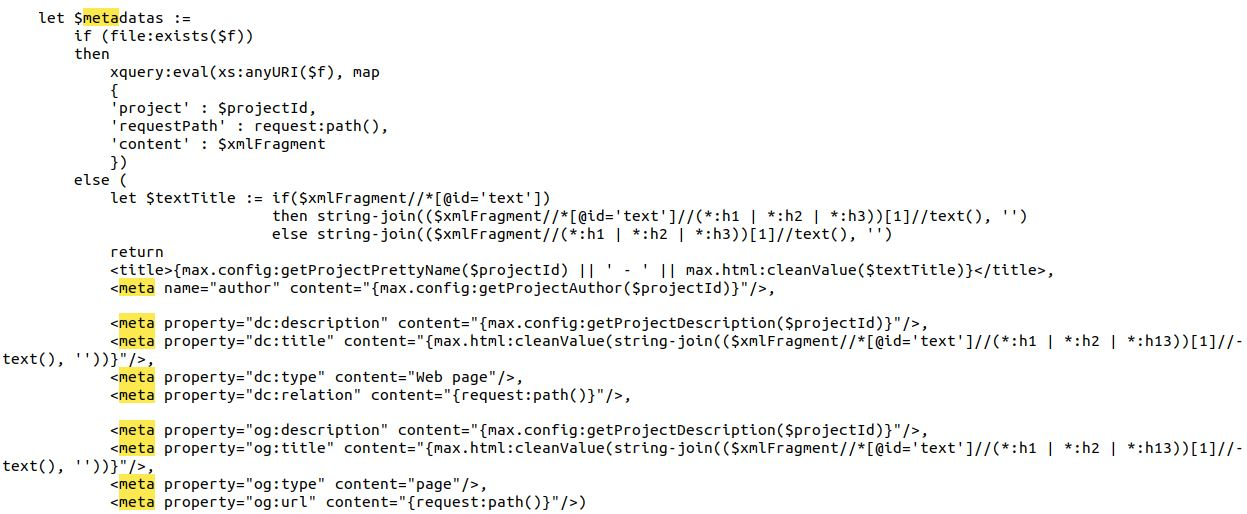
\includegraphics[width=15cm]{img/partie_2/metadata_max.JPG}
    \caption{Fichier de requêtes de création des métadonnées \acrshort{HTML}.}
    \label{metadata}
\end{figure}


Dans ce fichier, deux types de processus de récupération des métadonnées sont identifiables : \textit{dc}  et \textit{og}.

Le premier fait référence aux métadonnées sous format Dublin Core. Le Dublin Core est un vocabulaire de métadonnées pour la  descriptions de documents, développé par le DCMI (Dublin Core Metadata Initiative). Cette structure de métadonnées a pour but de \og fournir un socle commun d'éléments descriptifs suffisamment structuré pour permettre une interopérabilité minimale entre des systèmes conçus indépendamment les uns des autres\footcite{dublincore}\fg. Le vocabulaire Dublin Core se compose de quinze éléments de base (Title, Subject, Description, Source, Format, Type, Creator, Contributor, Publisher, Rights, Relation, Coverage, Language, Date et Identifier), chacun des élements étant relié à un identifiant de ressource universel (URI) prérenne\footnote{Les URI sont des espaces de noms qui permettent de donner un identifiant pérenne à une source en lui donnant un chemin précis, basé sur les url. La liste des termes et leurs URI correspondants sont accessibles à cette adresse : \cite{dcmi}}.


Les quinze éléments de Dublin Core peuvent être associés avec des qualificateurs afin de leur donner un contexte (exemple pour le tag dc:relation, on peut lui attribuer les éléments \textit{unqualified}, \textit{has version}, \textit{is part of} etc.)


Au sein de MaX, on retrouve quatre de ces quinze éléments :

\begin{itemize}
    \item \texttt{dc:description}, sorte de résumé de la source
    \item \texttt{dc:title}, pour le nom donné à la source
    \item \texttt{dc:type} donne le genre ou la nature de la source (image, article, musique etc...)
    \item \texttt{dc:relation}, pour décrire une source connexe
\end{itemize}

Au moment de la création d'une page web avec MaX, certaines métadonnées sont renseignées, mais seulement celles concernant le type et la relation, comme on peut le voir sur la figure \ref{dc_animal}. On voit même que dans ce dernier cas, l'élément \textit{dc:title} est erroné puisque la requête xQuery correspondante affiche toutes les valeurs des balises XML <title> et non pas seulement la valeur de la première comme voulu.

\begin{figure}[H]
    \centering
    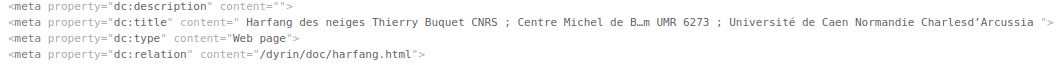
\includegraphics[width=\textwidth,height=\textheight,keepaspectratio]{img/partie_2/metadata_dc_animal.JPG}
    \caption{Métadonnées \acrshort{HTML} de la fiche animale du harfang des neiges.}
    \label{dc_animal}
\end{figure}


Le deuxième protocole de métadonnées suivi par MaX est celui de l'\acrfull{OGP} et s'inspire du Dublin Core. L'\acrshort{OGP} est un protocole de description de métadonnées créé par Facebook permettant aux pages web de se comporter comme des pages du réseau social et ainsi d'être facilement partageables sur ces mêmes réseaux (Twitter, Facebook, Linkedin...)\footcite{OGP}. Si ces métadonnées n'existent pas, les robots interpréteurs essaieront d'en créer d'eux mêmes, mais le résultat ne sera pas optimal.

Pour illustrer nos propos, prenons l'exemple des billets de blog du réseau social Twitter. La figure \ref{twitter} ci-dessous illustre l'organisation et la localisation de métadonnées utilisées. Dans cet exemple, le billet ne présente pas de problème d'affichage, ses métadonnées ayant bien été entrées. En revanche la figure \ref{bad_figure} suivante montre un problème d'affichage d'image. Si l'on regarde ses métadonnées renseignées en figure \ref{tag_og}, on remarque que le tag \texttt{og:image} est erroné, ne redirigeant pas vers une ressource physique (il manque le format de l'image en fin de valeur). L'interpréteur web ajoute alors de lui même une image générique symbolisant un problème d'affichage.

\begin{figure}[H]
    \centering
    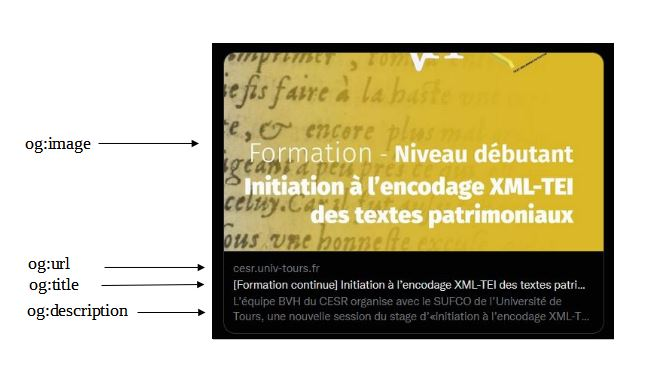
\includegraphics[width=12cm]{img/partie_2/exemple_og.JPG}
    \caption{Anatomie d'un billet Twitter utilisant des tags Open Graph bien formés.}
    \label{twitter}
\end{figure}


\begin{figure}[H]
    \centering
    
\includegraphics[width=12cm]{img/partie_2/poitiers.JPG}
    \caption{Dans cet exemple, le tag \texttt{og:image} n'a pas son format de renseigné. L'interpréteur a donc chargé de lui-même une image présentée par défaut dans cette situation.}
    \label{bad_figure}
\end{figure}

\begin{figure}[H]
    \centering
    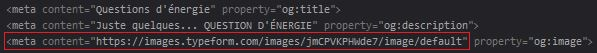
\includegraphics[width=12cm]{img/partie_2/og_image_bad.JPG}
    \caption{Le tag \texttt{og:image} avec un format manquant responsable du problème d'affichage}
    \label{tag_og}
\end{figure}


Il est donc important de veiller à remplir de manière la plus complète et juste possible les métadonnées des documents, afin que leur partage soit optimal.
Concernant ce protocole \acrshort{OGP}, MaX prend en charge quatre types de tag :

\begin{itemize}
    \item \texttt{og:title}, qui renseigne le titre de la page. Il vaut mieux ne pas dépasser les 65 caractères maximum, au risque de le voir tronqué à l'affichage.
    \item \texttt{og:desription}, qui correspond une description courte de la page. Il est recommandé de ne pas dépasser 300 caractères pour cette balise, pour un affichage optimal sur les réseaux sociaux.
    \item \texttt{og:url}, qui renvoie l'url canonique de la page. En général, elle est déjà affichée par le navigateur dans les résultats de recherche.
    \item \texttt{og:type}, qui donne le type de la page et qui décrit le type principal d'objet contenu dans celle-ci (article, vidéo, musique).
\end{itemize}

Sans aucune surcharge et sans aucune modification, MaX renvoie automatiquement des données associées à ces tags grâce aux requêtes prédéfinies du fichier \texttt{html.xqm}. On obtient le résultat \acrshort{HTML} ci-dessous :


\begin{figure}[H]
    \centering
    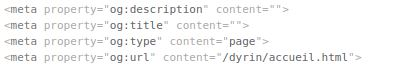
\includegraphics[width=10cm]{img/partie_2/og_test.JPG}
    \caption{Métadonnées \acrshort{HTML} de la page d'accueil créées par MaX dans Dyrin.}
    \label{meta_accueil}
\end{figure}


\begin{figure}[H]
    \centering
    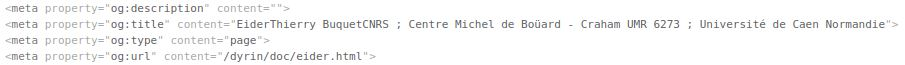
\includegraphics[width=15cm]{img/partie_2/og_test_eider.JPG}
    \caption{Métadonnées \acrshort{HTML} de la fiche animale de l'eider.}
    \label{meta_eider}
\end{figure}


On peut voir que ces métadonnées ne sont remplies que partiellement : il manque en effet des informations pour les tags \textit{og:description} et \textit{og:title} de la page d'accueil en figure \ref{meta_accueil}. Les requêtes qui y sont associées ne renvoient pas d'informations. De plus, les balises d'une page d'un article ne doivent en aucun cas être une description générale du site. Les métadonnées qui y sont associées doivent évoluer en fonction de la page visitée. Si nous prenons l'exemple de Dyrin, les métadonnées associées à la page d'accueil ne doivent pas être les mêmes que celles présente sur une fiche animale. Or, si l'on compare la figure \ref{meta_accueil} avec la \ref{meta_eider}, on remarque que seul le tag \textit{og:title} de la fiche animale a été ajouté, mais que la description de la page elle, reste manquante.


Il revient donc de modifier manuellement les requêtes xQuery afin que celles-ci produisent les métadonnées Dublin Core et OGP nécessaires. Le temps du stage ayant été imparti à la date d'écriture du présent rapport, cela pourrait notamment être une voie d'exploration et d'amélioration de l'outil MaX. Ces métadonnées sont modifiables en créant un fichier \texttt{metadata.xq} dans le dossier \texttt{[projet-]editions/[edition]/xq}. Il revient alors de créer ses propres requêtes xQuery pour en modifier le contenu. Or, comme nous le disions plus haut, il est essentiel d'avoir des métadonnées relatives à chacune des pages du site et non pas des métadonnées globales. Il faudra donc construire des requêtes en fonction des url interrogées. 

Une autre solution de référencement pérenne intéresse le \acrshort{PDN} : l'utilisation de DOI sur les pages des sites web. Un DOI (\acrlong{DOI}) est une solution permettant d'identifier, référencer, citer et fournir un lien durable à des ressources de toutes sortes (personnes, images, objets, pages web...) en attribuant à ces derniers toutes sortes de métadonnées. Les métadonnées sont des caractéristiques de description d'une source ou d'un objet : auteur, titre, résumé, date, liens, mots-clés, éditeurs, langues...Il s'agit d'une chaîne de caractère unique et pérenne dans le temps, puisqu'un DOI par mise-à-jour serait attribué\footcite{DOI}. \\
   Un DOI est facilement repérable car il porte toujours la même structure de fabrication. Il est composé d'une première partie attribuée par un organisme dédié tandis que la deuxième partie, derrière le signe \og /\fg est déterminée par le client. On peut retrouver cette structure avec l'exemple du DOI de l'article \og \textit{Éditer un cahier de travail de Montesquieu}\footcite{montesquieu}\fg{} dans le tableau \ref{DOI} ci-dessous :
   
   \begin{table}[H]
\centering
\begin{tabular}{|c|c|}
\hline
 \cellcolor{lightgray}Exemple de DOI : &  \textbf{10.4000/recherchestravaux.100} \\
\hline
\textit{partie 1} & \textit{10.4000} est la partie attribuée par l'agence attribuant les DOI \\
\hline
\textit{partie 2} & \textit{recherchestravaux.100} est la partie choisie par le client. \\
\hline
\end{tabular}
\caption{Tableau explicatif de la structure d'un lien DOI.}
\label{DOI}
\end{table}

L'adhésion à un organisme distributeur de DOI est payant, ce qui se justifie car cela permet d'éviter la profusion d'identifiants et de pouvoir en contrôler la réglementation, de même que de mieux regrouper les identifications. L'accès à la source est possible en tapant son DOI précédé de \texttt{doi.org/} directement dans la barre de recherche d'un navigateur. Des plugins pour chaque navigateurs existent également pour récupérer rapidement le DOI d'une source (exemple de l'application \og DOI resolver \fg de Google Chrome\footcite{doi-resolver}. Dans le cas d'une url, si celle-ci bouge ou vient à être supprimée, le DOI lui correspondant restera fixe de même que les informations qui lui sont associées. En résumé, attribuer un DOI à des pages web permettrait de stabiliser son contenu à un instant T afin de pouvoir le rendre accessible à tout moment, qu'importe le nombre de mises-à-jour postérieures. Cela nécessiterait probablement alors en plus, dans une politique d'accès facilité aux données, la création d'une sorte d'interface de navigation entre les DOI afin que ceux-ci soient facilement identifiables et exploitables par les utilisateurs.

\section{Reusable : documentation et après ?}
MaX est libre d'accès sur la page GitLab\footcite{pdn-certic} du \acrshort{CERTIC} avec sa documentation. Le logiciel est OpenSource et disponible gratuitement sous licence \acrshort{CECILL}- B\footcite{licences}, mention que l'on peut retrouver dans le fichier \texttt{legal.txt} de MaX. La licence CeCILL-B (\acrlong{CECILL}) est un type de licence attribuée aux logiciels développés en partenariat avec le \acrshort{CNRS} et l'\acrfull{INRIA}. La lettre B signifie que la licence a les caractéristiques d'une licence \acrfull{BSD} qui permet de réutiliser tout ou une partie du logiciel sans restriction\footcite{bsd}. Le libre accès à la ressource de même que l'indication claire de la licence utilisée par la ressource est un des axes principaux des principes FAIR. Dans la logique de sa diffusion, MaX est également accompagné d'une documentation élaborée par les membres du \acrshort{PDN} afin de rendre l'outil le plus facilement récupérable et utilisable possible. Malgré tout, cette mise à disposition pose plusieurs questions : tout d'abord la place du \acrshort{PDN} vis à vis de cette diffusion, notamment au niveau de l'aide fournie pour les personnes rencontrant des difficultés d'installation et d'utilisation. De l'expérience qui a été tirée au moment du stage effectué, plusieurs problèmes ont été soulevés. Un des objectifs du stage a été la prise en main de manière autonome de MaX afin de voir les éventuels soucis rencontrés. La documentation est certes d'une aide précieuse mais elle s'est montrée malheureusement insuffisante à certains moments de l'installation. Malgré tout, loin d'être un frein au développement, ces situations (relativement peu nombreuses) ont permis de parfaire la documentation. En conclusion, MaX reste relativement accessible. Accessible oui, mais à qui ?

Cette question peut-être illustrée par les journées SCRIPTO\footcite{scripto} ayant eu lieu au \acrshort{PDN} début juin 2022. L'objectif de ces journées étant une coopération entre les différentes \acrfull{MSH} de France dans l'optique d'échanger et de partager les pratiques de leurs membres. Deux journées au \acrshort{PDN} ont été organisées : une matinée était réservée pour la présentation des pratiques numérique du \acrshort{PDN}, tandis que l'après-midi portait sur un atelier d'installation de MaX. Les personnes présentes avaient le choix de travailler sur leur propre jeu de données ou bien de recevoir un jeu pré-existant. Avant les dites journées, la première étape avait été de se renseigner sur les compétences de chacun afin de les regrouper dans trois groupes : novice, intermédiaire et expert. Les critères de regroupement étaient axés selon l'expérience en ingénierie ainsi que les postes pourvus par chacun. Il est apparu que trois personnes n'avaient aucune expérience dans ce domaine, quatre personnes étaient dans le groupe intermédiaire et sept autres dans le groupe expert. Les discussions au \acrshort{PDN} ont alors tournées autour d'une question cruciale : à qui était destiné MaX ? Il s'agit bien d'un logiciel ouvert, mais ouvert vers qui ? En effet, comme il en est fait mention en première partie, il n'est pas nécessaire que l'utilisateur ait des connaissances très étendues en langage \acrshort{XSL} ou xQuery pour utiliser MaX. Cependant ce dernier s'installe tout de même à l'aide de commandes dans le terminal. Si les utilisateurs de Linux n'y verront pas de problème, c'est un peu moins le cas pour les utilisateurs de Mac et encore moins de ceux de Windows. La création d'outil et le choix du système d'exploitation sur lequel il tournera a des conséquences notables. Si les grandes sociétés éditrices de logiciels parviennent généralement à fournir des versions différentes pour chaque OS, les \acrshort{DSI} de taille plus raisonnable comme celle de l'université de Caen n'ont ni le temps ni les moyens de faire de même et doivent donc procéder à un choix. Il a donc été décidé de développer MaX uniquement sous Linux et Mac OS, mettant de côté les utilisateurs Windows. Pour les personnes qui seraient néanmoins intéressées par l'utilisation de MaX, il leur appartient de se former pour surmonter des obstacles techniques comme l'utilisation d'un terminal dans l'optique de développer des compétences qui pourront également leur être utiles dans d'autres projets. En ce qui concerne les journées SCRIPTO, la décision fut prise de faire des groupes de personnes de même niveau, épaulés par des membres du \acrshort{PDN} disposés à aider si le besoin s'en faisait sentir. Ce qui a très vite été le cas. L'idée selon laquelle la documentation seule était suffisante pour pouvoir se servir de MaX ne tenait plus. Cependant cette expérience doit-elle nous faire douter de la qualité, voire même de l'utilité de la documentation proposée ? Nous ne le pensons pas. Rappelons que cette documentation n'est pas toujours bien suivie et qu'il arrive aux utilisateurs, voulant aller trop vite, de sauter des étapes cruciales, ou bien encore de mal interpréter une instruction. Dans ce cas là il ne faut pas hésiter à reprendre l'installation du début et à faire preuve de patience\footnote{Comme aime souvent le rappeler avec ironie une connaissance ingénieur de longue date : \og Quand tout a échoué, lire la doc\fg.}.  Elle nous ramène cependant à la question de la place et du niveau d'investissement du \acrshort{PDN} dans la diffusion de MaX.



Il faut aussi souligner que cette documentation a été créée pour permettre au \acrshort{PDN} de se libérer du soucis de devenir un lieu de maintenance technique où les ingénieurs passeraient une bonne partie de leur temps à résoudre des problèmes d'installation à distance. Ce choix n'est pas pas fermé : dans le cas de \acrshort{METOPES} cette mission d'assistance est au c\oe{}ur de l'institution, dès lors leurs ingénieurs passent beaucoup de temps à la formation et au soutien technique de leurs partenaires, autant à distance que via des formations dispensées dans toute la France. Le choix de ne pas suivre cette voie a été pris au \acrshort{PDN} afin de pouvoir laisser le plus de temps possible aux ingénieurs à la recherche et à l'innovation, afin que le \acrshort{PDN} puisse tenir son rôle de laboratoire de recherche d'édition de sources numériques.

Une autre question s'est posée au moment de la sortie de MaX, début avril : est-il nécessaire de communiquer dessus ? Si oui, comment s'y prendre ? L'idée de faire une annonce sur la liste de diffusion DH\footnote{DH est une liste de discussion francophone concernant les Digital Humanities (DH), ouverte à toutes les disciplines de sciences humaines et sociales. Elle fait partie des services offerts par \textit{Humanistica}, l'association francophone des humanités numériques. \cite{dh}}, dans un premier temps attractif, a cependant été repoussée. En effet un des \og risques\fg{} encouru par le \acrshort{PDN} aurait été de se voir dépassé par des demandes d'installation auxquelles il ne serait pas possible de répondre. Pour cette raison l'idée a été abandonnée. En ce qui concerne le déploiement de MaX, une des solutions envisagée dans ce cas est probablement d'effectuer des temps de formation comme ceux ayant eu lieu lors des journées SCRIPTO, probablement sur une journée entière à raison d'une fois par an, dans l'optique de donner des compétences solides à des ingénieurs extérieurs qui pourront par la suite diffuser ces pratiques au sein de leurs propres institutions.


\section{Prévenir des questions de maintenance}\label{bootstrap}
Un des autres grands enjeux dans la diffusion d'un outil est donc sa maniabilité et sa maintenance sur le long terme. Afin que celui-ci puisse être fonctionnel le plus longtemps possible, il est important d'essayer de le rendre le plus simple d'un point de vue technique permettant de pouvoir garder dessus un certain contrôle.

Pour illustrer cela nous pouvons prendre en exemple le revirement du \acrshort{PDN} autour de certaines technologies qui étaient utilisées au temps où les projets étaient produits non pas par MaX, mais par le logiciel PLEADE\footcite{pleade}. Ce dernier, développé en OpenSource, est un logiciel à destination des archives, bibliothèques et musées qui permet la valorisation des données patrimoniales pour un objectif de publication, diffusion et de dissémination de ces données\footcite{pleade}. L'outil ayant récemment montré des failles de sécurité dans son système (\textbf{retrouver l'article en question...}), la décision a été prise de migrer tous les projets du \acrshort{PDN} vers MaX. Ce qui a également permis un plus grand contrôle technique pour les ingénieurs du \acrshort{PDN} qui ne dépendaient plus des mises-à-jour et des bugs techniques induits par PLEADE. Lors de la création de MaX, l'idée de limiter l'outil à son strict minimum technique a été de plus en plus confirmée permettant notamment aux ingénieurs du \acrshort{PDN} de réduire considérablement le temps de maintenance de la soixantaine de projet existant.

\subsection{Suppression de jQuery}
Une des premières et des plus grandes décisions à avoir été prise à ce sujet est la suppression des briques techniques jQuery et Bootstrap. JQuery est une bibliothèque JavaScript libre et multiplateforme créée en 2006 dans le but de faciliter l'écriture de scripts côté client dans le code \acrshort{HTML} des pages web. Cette bibliothèque permettait notamment le parcours et la manipulation sans précédent du \acrfull{DOM}\footnote{Le document object model est la représentation sous forme d'objets (de choses) du code de la page \acrshort{HTML}. C'est aussi une convention qui permet de manipuler les éléments d'une page Web. Le langage JavaScript qui parcourt une page Web la comprend comme une collection d'objets organisés selon une hiérarchie logique. Le DOM obéit à une structure en arbre (l'élément \acrshort{HTML} étant à la racine) où chaque élément appelé n\oe{}ud peut contenir d'autres éléments (enfants). \cite{dom_2020}}. Elle contient en effet de nombreuses fonctionnalités : gestion des animations, de la manipulation des feuilles CSS, gestion des évènements, etc. Un des points intéressants de jQuery à l'époque de sa création était qu'il permettait de réduire les écarts de traitement entre les différents navigateurs qui agissaient de manière indépendante. Or cet écart se réduit de plus en plus, comme nous le montre le groupe de travail intitulé
\acrfull{WECG}\footnote{Il s'agit d'un groupe de travail mis en place par le collectif W3C.} qui cherche actuellement à mettre en place une standardisation des navigateurs Apple, Google, Microsoft et Mozilla\footcite{webextensions}. Par conséquence, le recours à jQuery peut être remis en question. De plus, les nombreux plugins intégrés à jQuery ont posé des problèmes lors de leur mise-à-jour, quand ils n'ont pas tout simplement été supprimés. C'est un aspect mis en avant sur le site officiel de jQuery :

\begin{otherlanguage}{english}
\begin{quote}
    \textit{The quality of jQuery plugins varies widely. Many plugins are extensively tested and well-maintained, but others are hastily created and then ignored. More than a few fail to follow best practices}\footcite{jquery}.
\end{quote}
\end{otherlanguage}

Insérer du jQuery dans son projet signifie devoir très souvent vérifier la conformité et la validité dudit plugin installé. Si cela reste possible à l'échelle d'un projet, un nombre de projets trop important risque de devenir extrêmement chronophage à maintenir dans le temps. Et les mises-à-jour ne doivent pas être optionnelles : elles ont en réalité pour fonction de corriger toutes les vulnérabilités en matière de cybersécurité\footcite{security}, et sont donc extrêmement importantes.

\subsection{Suppression de Bootstrap}
C'est la même réflexion qui a poussé à la suppression de la technologie Bootstrap. Développé en 2011, Bootstrap est un framework contenant des codes \acrshort{HTML} et CSS, des formulaires, boutons, outils de navigation et autres éléments interactifs, ainsi que des extensions JavaScript en option. À l'instar de jQuery il permet d'ajouter des codes préconçus pour le design de ses sites web sans avoir réellement besoin d'éditer soi-même les feuilles CSS. Plusieurs problèmes se posent avec cette technologie : tout d'abord son poids, un peu moins de 600ko. Si cela reste très relatif, la technologie était cependant auparavant liée à celle de jQuery et nécessitait également son téléchargement\footcite{why-bootstrap}, même si ce n'est plus le cas depuis la version 5 de 2020. Bien que cette dépendance n'existe plus, elle pose la question de l'interdépendance des briques technologiques entre elles.

Elle pose aussi la question de la souveraineté de ce genre de technologies dans un sens où ces dernières, dans leur objectif de rester attractif, font le choix d'abandonner une partie de leurs utilisateurs en route en multipliant les mises à niveau. En effet la version 5 de Bootstrap a récemment fait le choix d'abandonner son support pour les navigateur Internet Explorer 10 et Internet Explorer 11, ce qui pose des questions sur l'obsolescence de ces logiciels incompatibles avec des versions antérieures\footcite{themesberg_bootstrap}.

 Un dernier problème vis à vis de Bootstrap est que malgré son apparente facilité d'utilisation, son code n'est pas si aisément adaptable et modifiable à souhait. Certains de ses paquets présentent parfois une écriture trop complexe pour être reprise par soi-même. Il est même parfois plus rapide d'éditer sa propre feuille CSS que de reprendre celle de Bootstrap. Un problème similaire s'est présenté avec les fichiers CSS dans MaX: chaque partie du site Web faisant appel à un fichier CSS particulier, il était parfois difficile d'arriver au rendu souhaité sans avoir à éditer les fichiers CSS sois disant intouchables du \og c\oe{}ur\fg{} de MaX.


Cependant, s'il a été jugé préférable de ne plus utiliser Bootstrap au \acrshort{PDN}, cela ne revient pas à dire qu'il faut totalement en banir l'utilisation à tous les niveaux. Il faut se poser les bonnes questions afin de juger à quel moment l'utilisation de Bootstrap est-elle une plus value : vais-je devoir en utiliser plusieurs composants ? Suis-je vraiment dans un besoin pressant de développer le design de mon site maintenant, ou au contraire, cela peut-il attendre un développement plus long pour du sur-mesure fait main ? Et surtout la question suivante : ai-je véritablement de ce composant dans mon projet ? Quelle est, si elle existe, sa véritable part de valeur ajoutée ? Et que se passe-t-il si je ne l'intègre pas ? Tous ces questionnements semblent peut-être anecdotiques. Néanmoins ils ont pour mérite de permettre une réflexion au moment du développement afin de véritablement creuser la question du \textit{pourquoi} et non plus simplement du \textit{comment}. Une sorte de première prise de recul qui nous font nous poser des questions cruciales concernant l'avenir du numérique.

\part{Le projet Dyrin}

\chapter{Objectifs scientifiques de Dyrin}
Les objectifs scientifiques de Dyrin sont de plusieurs natures : la création d'une conséquente base bibliographique relative à la faune du Nord, présentant une structure singulière et réfléchie, répondant à des enjeux scientifiques que nous allons détailler ici. La figure \ref{structure} ci-dessous offre une aide à la visualisation quant aux différents traitements ayant lieu dans Dyrin.

\begin{figure}[H]
    \centering
    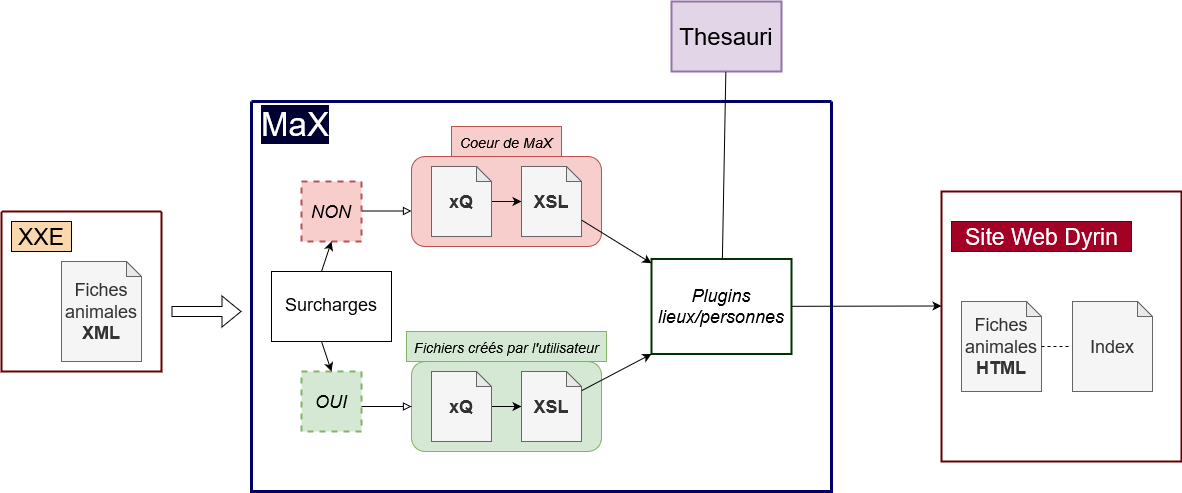
\includegraphics[width=\linewidth]{img/partie_3/schema.png}
    \caption{Structure de traitement de la chaîne éditoriale de Dyrin.}
    \label{structure}
\end{figure}

\section{La structure}
Le choix de structure reflété par le site de Dyrin n'est pas imposé par MaX. Certes Dyrin respecte bien dans sa structure fonctionnelle les trois dossiers distincts \texttt{[projet]-BaseX}, \texttt{[projet]-editions} et \texttt{[projet]-MaX}. Mais par les nombreuses surcharges qui ont été ajoutées, Dyrin propose une manière singulière d'afficher ses données XML. Il s'agit de la volonté du porteur de projet qui a aboutit à la création d'un site unique, à des fins scientifiques particulières. 

Le site Web de Dyrin constitue une base de données bibliographiques (sources, études, iconographie) relative à cette faune du Nord (ours polaire, morse, narval, baleines, autres animaux et monstres marins, mais aussi faucons gerfauts, rennes, élans, petits animaux à fourrure, etc.). Il ne s'agit pas d'une encyclopédie, ni d'une base textuelle de sources mais bien d'une bibliographie. Dyrin propose un outil orienté \og recherche \fg, permettant aux étudiants et aux chercheurs d'accéder à une bibliographie la plus complète possible sur chaque animal, mais aussi de pouvoir consulter les sources en ligne ; il s'agit donc d'une sorte d'\og atelier du chercheur \fg, permettant, à partir d'une liste de références de consulter des référentiels, des sources en ligne, d'importer des références bibliographiques, etc. La version actuelle du site créée est un démonstrateur : il ne comporte qu'au total onze fiches d'espèces animales, la plupart incomplètes dans leur contenu. Il s'agit avant tout d'un jeu de test qui a permis de valider les choix d'encodage, de normalisation et d'indexation. Le projet final devrait en comporter pas moins d'une cinquantaine, selon la sélection du chercheur Thierry Buquet.

Le site est structuré de la manière suivante :

\begin{itemize}
    \item une page \textit{Accueil} donnant les détails du projet, notamment son but scientifique.
    \item une page \textit{Sommaire} listant alphabétiquement les fiches animales disponibles.
    \item une page \textit{Index} dirigeant vers des pages d'index de lieux, personnes, auteurs, artistes, thèmes et de zoonymes.
    \item une page \textit{À propos} donnant des détails sur le contexte de mise en place du projet entre le \acrshort{PDN} et le \acrshort{CRAHAM}.
    \item une page \textit{Contacts} avec les coordonnées des différents porteurs du projet.
\end{itemize}


\section{Fiche animale : une découverte en quatre parties}

La structure d'une fiche d'animal se compose de quatre grandes parties : 

\begin{itemize}
    \item une première partie de présentation de l'animal contenant les divers zoonymes et références zoologiques de l'espèce, ainsi qu'une brève présentation zoologique et zoo-historique.
    \item une seconde partie présentant une liste bibliographique zoo-historique composée de référentiels.
    \item une troisième partie détaillant les sources antiques, médiévales et modernes spécifiques à l'espèce et consultables en lignes.
    \item une dernière partie recensant diverses ressources iconographiques.
\end{itemize}

\subsection{Zoonymes}
La première partie sur les zoonymes classe ces derniers en fonction de leur provenance d'une langue moderne (anglais, suédois, français, allemand...) ou bien ancienne (ancien français, latin, vieux norois...). Certaines formes sont accompagnées d'explications étymologiques proposées par le chercheur.

\begin{figure}[H]
    \centering
    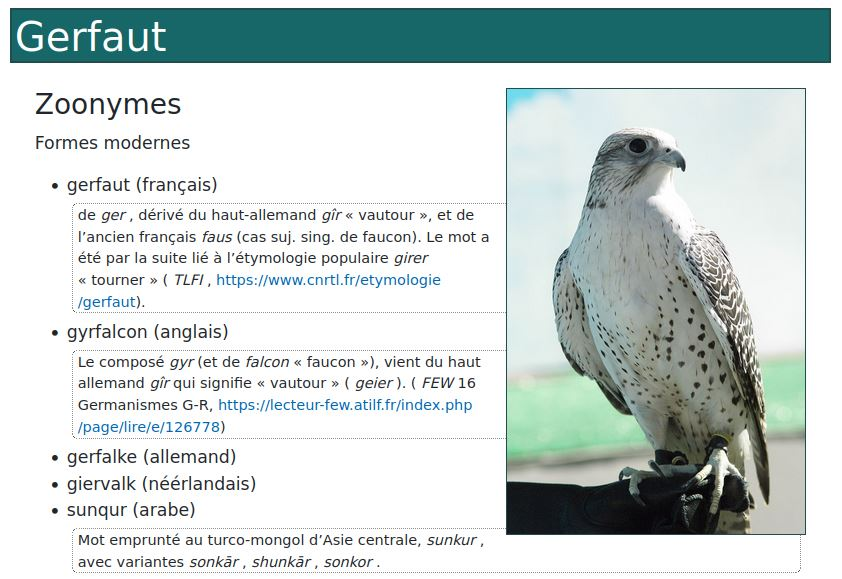
\includegraphics[width=12cm]{img/partie_3/gerfaut.JPG}
    \caption{Partie des zoonymes de la fiche animale sur le gerfaut.}
    \label{gerfaut}
\end{figure}

Dans la figure \ref{gerfaut} ci-dessus, on peut voir une partie des zoonymes attribués au gerfaut. Certains zoonymes peuvent être accompagnés de notes explicatives comprenant également le lien de la source. Par exemple pour le gerfaut, les zoonymes français (\textit{gerfaut}) et anglais (\textit{gyrfalcon}) sont accompagnés d'une note explicative étymologique comportant un extrait ainsi que des liens url vers des référentiels étymologiques. On retrouve le portail lexical de Ortolang\footcite{ortolang} référençant le \acrfull{TLFI}, version informatisée du dictionnaire du Trésor de la langue française\footnote{Le Trésor de la langue française (TFL) est un dictionnaire des XIX\textsuperscript{e} et XX\textsuperscript{e} siècles composé de 16 volumes contenant la définition de 100 000 mots avec leur histoire, 270 000 définitions et 430 000 exemples. \cite{tlfi}}, ou bien encore le \acrfull{FEW}, dictionnaire étymologique et historique du galloroman. Cette vision étymologique large permet de voir les relations historiques et géographiques entre les différents termes. Il est spécifié par exemple plus bas dans la fiche (que l'on ne voit pas dans la figure ci-dessus) que le terme ancien \textit{geirfalki} en vieux norrois n'est attesté dans les langues nordiques qu'à partir du \textsc{xii}\ieme{} siècle, ce qui peut donner une première fourchette chronologique à la domestication ou à l'importation de l'animal en Scandinavie.


Au sein de cette partie on trouve également une sous partie traitant des références et référentiels zoologiques, comme on peut le voir dans la figure \ref{ref_zoo} ci-dessous :

\begin{figure}[H]
    \centering
    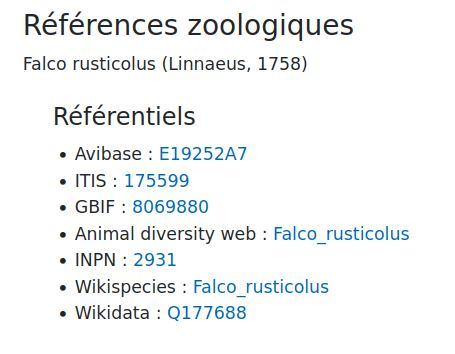
\includegraphics[width=6cm]{img/partie_3/ref_zoo.JPG}
    \caption{Références zoologiques de la fiche animale du gerfaut.}
    \label{ref_zoo}
\end{figure}

Ces référentiels zoologiques sont des redirections vers d'autres sites et bases zoologiques mondiales comme par exemple la base ornithologique Avibase, ou l' \acrfull{ITIS}\footnote{La ITIS est une association créée pour fournir des informations conformes et fiables sur la taxonomie des espèces biologiques. \cite{taxonomie}} ou bien encore la base \acrfull{ADW}\footnote{La ADW une base de données en ligne qui recueille l'histoire naturelle, la classification, les caractéristiques des espèces, la biologie de la conservation et les informations de distribution sur des milliers d'espèces d'animaux. Le site Web comprend des milliers de photographies, des centaines de clips sonores et un musée virtuel. \cite{adw}}. On y trouve également le nom scientifique de l'espèce donné par le classement du naturaliste suédois Carl von Linné qui, au \textsc{xviii}\ieme{} siècle, a posé les bases du système moderne de la nomenclature binominale\footnote{En taxinomie (botanique, zoologie, mycologie, etc.), le nom binominal est une combinaison de deux mots servant à désigner une espèce. Le premier mot, le nom générique, circonscrit un genre ; le second, l'épithète spécifique, indissociable du nom générique, sert à désigner l'espèce au sein de ce genre. \cite{binomial}}. Afin d'éviter que les url de ces sites soient trop visibles et surchargent l'espace graphique, il a été décidé de ne pas les dévoiler entièrement mais de les associer aux derniers termes de l'attribut XML \texttt{@target}, comme le montre la figure \ref{url} ci-dessous.

\begin{figure}[H]
    \centering
    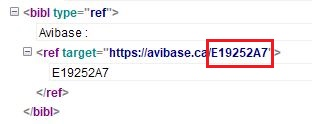
\includegraphics[width=6cm]{img/partie_3/zoo_xml.JPG}
    \caption{Encadré en rouge, l'url correspondante à la base ornithologique \textit{Avibase} que l'on retrouve dans les référentiels.
    }
    \label{url}
\end{figure}


À la suite des références se trouve une présentation zoologique ainsi qu'une bibliographie d'où est tirée cette présentation. Ainsi dans l'exemple ci-dessous \ref{pres_zoo} :

\begin{figure}[H]
    \centering
    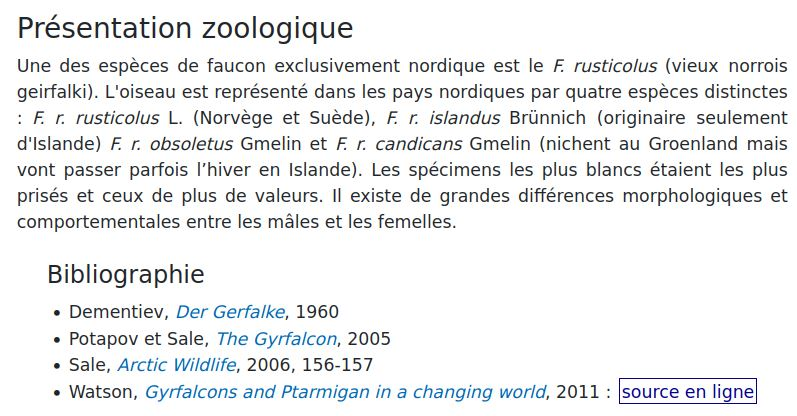
\includegraphics[width=10cm]{img/partie_3/pres_zoo.JPG}
    \caption{Exemple d'une présentation zoologique tirée de la fiche animale du gerfaut.}
    \label{pres_zoo}
\end{figure}

Dans cette image, on peut voir la présentation zoologique rédigée par l'auteur de la fiche, Thierry Buquet. L'objectif est de décrire succinctement l'animal tout en donnant les références bibliographiques correspondantes. Cette bibliographie est aussi une porte d'accès à une bibliographie en ligne Zotero : l'action de cliquer sur une des url présente provoque l'apparition d'une fenêtre pop-up reliée à l'application Zotero, comme le montre l'exemple de la figure \ref{partie_zotero} ci-dessous. La balise \acrshort{HTML} <url> attribuée à \textit{Artic widlife} renvoie à des informations quant à l'ouvrage au titre complet \og \textit{A complete guide to Artic widlife}\fg. La fenêtre de Zotero (visible dans la figure suivante \ref{zotero-pop}) nous donne accès aux différentes caractéristiques de l'\oe{}uvre en question (titre, auteur, lieu de publication et de conservation, url de la version numérisée si elle existe etc.).

\begin{figure}[H]
    \centering
    \includegraphics[width=12cm]{img/partie_3/zotero.JPG}
    \caption{Une pop-up de l'application Zotero s'affiche lorsqu'une url de la bibliographie est activée.}
    \label{zotero-pop}
\end{figure}

Enfin, comme dernière sous-partie à cette première partie, on trouve une description zoo-historique de l'espèce. Contrairement à la présentation zoologique, qui est une description biologique, la présentation zoo-historique donne quant à elle des informations sur les connaissances historiques et culturelles liées à la découverte voire à la domestication de l'animal. Il peut s'agir notamment d'informations quant aux pratiques de chasse, d'élevage ou bien encore de récits fantastiques. L'exemple de la figure \ref{zoo_histo} ci-dessous rapporte le rôle et la place du gerfaut comme cadeau prestigieux.

\begin{figure}[H]
    \centering
    \includegraphics[width=13cm]{img/partie_3/pres_zoo_hist.JPG}
    \caption{Exemple de présentation zoo-historique du gerfaut.}
    \label{zoo_histo}
\end{figure}

\subsection{Bibliographie zoo-historique}
La seconde grande partie des fiches animales est consacrée à une bibliographie zoo-historique. On y trouve des référentiels bibliographiques dans lesquels sont donnés les noms des bibliothèques numériques de références. En continuant de prendre l'exemple du gerfaut, on peut se référer à la figure \ref{ref_biblio} ci-dessous dans laquelle on trouve une référence faite à la bibliothèque \textit{Animaliter}, plus particulièrement à la page des faucons (\textit{Falke}) qui recense près d'une centaine d'ouvrages et de documents sur le gerfaut. La bibliographie sur l'histoire de l'animal quant à elle, redirige sur des références Zotero de la base Dyrin.

\begin{figure}[H]
    \centering
    \includegraphics[width=12cm]{img/partie_3/biblio.png}
    \caption{Exemple de bibliographie zoo-historique de la fiche animale du gerfaut.}
    \label{ref_biblio}
\end{figure}

Certaines références sont accompagnées de notes de recherches ainsi que d'hyperliens vers lesdites ressources lorsque celles-ci sont disponibles. Une chose reste très importante vis-à-vis de ces sources : la mention de leur licence, indispensable à cette volonté de centralisation des références bibliographiques et de mise en valeur des ressources en accès-libre dans une logique de partage des savoirs. Ces licences sont inscrites de manière visible dans une politique de transparence vis-à-vis de l'utilisateur et des institutions productrices de ces sources. On retrouve la mention de licence payante dans Dyrin sous le terme de \textit{paywall} que l'on retrouve à côté de la source concernée. Un exemple nous est donné dans la figure \ref{biblio_notes}. Une source ne portant pas cette information est considérée comme étant une ressource libre d'accès. La grande majorité des sources indiquées dans Dyrin sont en accès libre, ce qui favorise leur partage et leur diffusion.

\begin{figure}[H]
    \centering
    \includegraphics[width=12cm]{img/partie_3/biblio_notes.png}
    \caption{Exemple de mention d'une mention de licence payante \textit{paywall}.}
    \label{biblio_notes}
\end{figure}

\subsection{\OE{}uvres textuelles}
La troisième grande partie concerne une description des \oe{}uvres textuelles où l'on retrouve une mention de l'animal, classées de manière périodique : antiquité, moyen-âge et moderne. En voici un exemple dans la figure \ref{sources} suivante :

\begin{figure}[H]
    \centering
    \includegraphics[width=12cm]{img/partie_3/oeuvre.png}
    \caption{Exemple d'une structuration d'une \oe{}uvre tirée de la fiche du gerfaut.}
    \label{sources}
\end{figure}

Chaque \oe{}uvre se présente de la façon suivante, quelque soit l'époque historique, comme illustré dans la figure \ref{template} ci-dessous : 

\begin{figure}[H]
    \centering
    \includegraphics[width=10cm]{img/partie_3/template.JPG}
    \caption{\textit{Template} de citation d'une \oe{}uvre.}
    \label{template}
\end{figure}

Une typographie particulière est associée à chaque élément. L'auteur apparaît dans une police d'une taille plus grande que celle des autres éléments et de couleur bleue. Suivi du titre de l'\oe{}uvre, de son type et de la langue dans laquelle elle est rédigée. Le dernier élément est la date de rédaction. On trouve en dessous une liste de mots clés dont chaque couleur fait référence à une catégorie particulière d'index : 
\begin{itemize}
    \item lieux (vert)
    \item thèmes (orange)
    \item zoonymes (bleu foncé)
    \item personnes (bleu clair)
    \item animaux (gris)
    \item analytique (rouge foncé)
\end{itemize}
Ces mots clés sont très précieux car ils sont des portes d'entrée aux pages d'index regroupant ces derniers par thèmes. Le nom de l'auteur est aussi une redirection vers l'index des personnages. À la suite de cette description, on trouve les différentes éditions disponibles pour cette \oe{}uvre. Les titres des \oe{}uvres sont reliés à la bibliothèque numérique Zotero (voir partie \ref{partie_zotero}) et sont parfois suivis d'un lien url classique vers la ressource numérique bien dans un format d'images \acrshort{IIIF}. Ce lien \acrshort{IIIF} permet l'ouverture, de la même manière que pour Zotero, d'une fenêtre indépendante de visualisation d'images, comme le montre la figure \ref{mirador-iiif} suivante :

\begin{figure}[H]
    \centering
    \includegraphics[width=\linewidth]{img/partie_3/mirador.png}
    \caption{Ouverture d'une fenêtre de visualisation d'image \acrshort{IIIF} par la visionneuse Mirador.}
    \label{mirador-iiif}
\end{figure}

Cette visionneuse Mirador permet de visualiser les numérisations d'ouvrages ou articles recensés dans les fiches \acrshort{XML} animales.

\subsection{Iconographie}
Enfin, la dernière grande partie de cette structure correspond à une sélection de liens pointant vers des ressources en ligne en accès ouvert, en donnant la priorité aux données en \acrshort{IIIF}. Cela donne la possibilité de pouvoir de consulter un extrait en contexte, par la consultation de l'ouvrage source en haute définition.

\begin{figure}[H]
    \centering
    \includegraphics[width=12cm]{img/partie_3/icono.JPG}
    \caption{Exemple de la partie iconographie de la fiche du narval.}
    \label{icono}
\end{figure}

Cette section iconographie est présentée ci-dessus dans la figure \ref{icono}. Chaque image comporte un titre donné par l'auteur de la fiche, suivi de la date de création de la ressource. On trouve ensuite le lien Zotero vers l'institution de conservation. Le ou les auteurs des \oe{}uvres sont indiqués en dessous et sont reliés à leur fiche descriptive Thesauri\footnote{Le fonctionnement de ces Thesauri est détaillé plus bas en \ref{thesauri}}. En dessous sont indiqués les liens des ressources, dans un format de haute qualité \acrshort{IIIF} ou bien via un hyperlien url. On donne ensuite des détails sur la nature de la ressource ainsi qu'une brève description.\\


En conclusion, nous voyons que la présentation des animaux dans Dyrin est le fruit d'une réflexion sur l'organisation de la donnée de manière optimisée  : on retrouve quatre grandes parties (présentation, bibliographie, ressources textuelles, ressources iconographiques) répondant à des objectifs scientifiques précis.

Tout d'abord celui de créer une base bibliographique ordonnée et efficace : chaque fiche animale propose une structure identique aux autres, facilitant la compréhension et le repérage dans les informations présentées. Cette même structure a été pensée pour offrir à l'utilisateur une vision dense mais diversifiée de l'histoire de ces animaux du Nord à travers différentes thématiques (géographie, histoire, biologie...). Des mots clés sont attribués à chacune des \oe{}uvres afin de pouvoir rapidement repérer les thématiques abordées.

Le site de Dyrin permet de rassembler en un lieu commun des points de savoirs qui étaient auparavant dispersés en ligne. La construction d'un site Web a également été le moyen de montrer et de diffuser une bibliothèque numérique Zotero de taille conséquente.


\section{Zotero : une bibliothèque collaborative et partageable}\label{partie_zotero}

Zotero est un logiciel de gestion de références bibliographiques gratuit, libre et OpenSource dont la première version est sortie en 2006. L'outil dans sa version classique est gratuit et téléchargeable pour tous les systèmes d'exploitation. Depuis Zotero, on trouve la possibilité de créer des bibliothèques de groupe, ce qui permet une collaboration sur les bibliographies. De plus, trois types de bibliothèque de groupe existent :
\begin{itemize}
    \item privé ;
    \item public en accès restreint pour la modification ;
    \item public en accès ouvert pour la modification ;
\end{itemize}
Dyrin utilise cette fonctionnalité pour exposer la bibliographie du projet, et la rendre accessible de façon structurée. Les références sont ainsi importables dans une instance Zotero ou tout autre outil de gestion bibliographique.

\begin{figure}[H]
    \centering
    \includegraphics[width=\linewidth]{img/partie_3/zotero_dyrin.JPG}
    \caption{Capture d'écran de la bibliothèque numérique de Dyrin dans l'application Zotero.}
    \label{zoterogui}
\end{figure}

Le logiciel, dont on peut retrouver une capture d'écran ci-dessus en figure \ref{zoterogui} se présente sous l'aspect d'une fenêtre découpée en trois colonnes. 


\begin{enumerate}
    \item Celle de gauche montre la structure de dossiers et de sous-dossiers toujours en cours de composition, du projet Dyrin. Dans un premier dossier intitulé \texttt{00\_notices\_en\_cours} on trouve la liste des notices bibliographiques qui nécessitent encore d'être classées. Dans le dossier \texttt{01\_General} on retrouve toutes les entrées de la bibliographie, peu importe leur place de classement. Puis dans un troisième dossier \texttt{02\_Sources} se trouvent les références bibliographiques classées selon leur langue ou leur période historique. Il existe également un autre dossier intitulé \texttt{08\_Fishing}, que l'on ne voit pas sur la figure, où sont situés les articles relatifs à la pêche, tandis que ceux traitant de la chasse sont dans un dossier \texttt{09\_Hunting}...au total ce ne sont pas moins de seize dossiers, classés par thématique, contenant chacun des ouvrages, articles et dossiers référencés. Dans cette même colonne, on retrouve en bas à gauche un formulaire de recherche selon les mots clés ayant été attribués aux documents.
    \item Au centre de la figure, on retrouve le détail des références entrées dans la bibliothèque numérique. Chacune porte un titre, un nom d'auteur et une date d'ajout. Chaque entrée est accompagnée d'un logo faisant référence au type de document enregistré : un ouvrage pour un livre dans son intégralité, un ouvrage ouvert pour un chapitre de livre, une page texte pour un article, un fichier PDF pour un document en version PDF, etc.
    \item À droite se trouvent les caractéristiques du document sélectionné : il est possible d'y recenser le type, le titre, les auteurs, le numéro et nom de collection, le nombre de volumes, les pages concernées, l'url ou le DOI renseignés, la date de consultation... Aucune de ces catégories n'est obligatoire mais l'intérêt d'une bibliothèque numérique, nous y reviendrons plus tard, est la fiabilité et la justesse des éléments qui y sont référencés. 
\end{enumerate}

S'il est possible de remplir les documents et leurs caractéristiques manuellement, il existe néanmoins une autre méthode plus \og rapide\fg. En effet Zotero donne la possibilité d'être téléchargé comme une extension de navigateur afin de pouvoir récupérer directement les métadonnées correspondantes aux sites et articles en ligne. Cela est rendu possible par plus de 600 scripts \textit{translators} incorporés dans Zotero, chacun d'entre eux référençant un site Web en particulier\footcite{translators}. Le compte Github de Zotero met à disposition l'intégralité de ces \textit{translators}\footcite{githubzotero}.

Si on prend l'exemple d'un article du chercheur Thierry Buquet intitulé \og 
\textit{Les informations relatives à la faune du Nord dans le Liber de natura rerum de Thomas de Cantimpré}
\fg, et que l'on clique sur l'outil d'extension de navigateur, une fenêtre apparaît comme sur la figure ci-dessous \ref{zotero_ext} :

\begin{figure}[H]
    \centering
    \includegraphics[width=\linewidth]{img/partie_3/zotero_navig.png}
    \caption{Encadrée en rouge, la fenêtre pop-up de récupération de métadonnées d'articles de
    Zotero.}
    \label{zotero_ext}
\end{figure}

Cette fenêtre nous propose alors d'enregistrer le document dans la bibliothèque numérique de notre choix. Une fois le choix validé, on peut retrouver le document en question dans l'application, comme nous le montre la figure \ref{zotero_article} ci-dessous : 


\begin{figure}[H]
    \centering
    \includegraphics[width=15cm]{img/partie_3/zotero_article.JPG}
    \caption{L'article et ses métadonnées sont ajoutés automatiquement dans la bibliothèque numérique.}
    \label{zotero_article}
\end{figure}


L'article que l'on voit encadré en rouge a été ajouté automatiquement à la base Zotero, tandis que ses métadonnées, encadrées en bleu, ont été intégrées dans le descriptif.
Si cela semble une manière plus simple et plus rapide de créer sa bibliothèque numérique, il semble bon de rappeler que cette efficacité n'est possible que si les métadonnées associées ont été décrites de manière très fine en amont. Un article, un ouvrage ou un PDF dont les métadonnées ont été mal décrites devra obligatoirement être repris au moment de l'intégration dans Zotero. Cela a été d'ailleurs une grosse partie du travail effectué lors du stage en M1 au \acrshort{CRAHAM} : la récupération et la reprise de documents intégrés dans la bibliothèque Zotero de Dyrin afin de pouvoir harmoniser et affiner les entrées.


Un des objectifs du projet Dyrin était donc la création de cette grande bibliographie participative sur Zotero, accessible librement à la consultation pour tous. Une des portes d'entrée de cette bibliographie étant les liens référencés dans les parties bibliographies des fiches animales.\\



\chapter{Exploration et améliorations techniques}
\section{L'exemple des plugins de Dyrin}
Comme nous le disions plus haut en \ref{plugin} lors de la description du fonctionnement de MaX, ce dernier est téléchargé accompagné de treize plugins correspondant chacun à une fonctionnalité supplémentaire au noyau de l'application MaX. Au sein du projet Dyrin, trois plugins sont activés : \texttt{thesauri\_pdn}, \texttt{index} et \texttt{mirador\_viewer}. Dans les passages suivants nous détaillerons les caractéristiques ainsi que spécificités de chacun d'eux pour ensuite nous intéresser à la manière dont ces briques technologiques ont été transformées et adaptées de manière particulière au projet.

\subsection{Dictionnaires collaboratifs : le plugin thesauri\_pdn}\label{thesauri}
Le terme de \textit{Thesauri} est le pluriel de \textit{Thesaurus}, mot latin donné à des lexiques de philologie ou d'archéologie, notamment à des dictionnaires exhaustifs, comprenant le vocabulaire complet d'une langue\footcite{def_thesau}. En résumé, les Thesauri sont des bases de données codifiées et unifiées permettant de regrouper en un seul lieu des fiches d'identité sur des thématiques particulières. Au \acrshort{PDN} ces Thesauri sont de trois types : \textit{personnes}, \textit{lieux} et \textit{\oe{}uvres}\footcite{thesauri}

\begin{figure}[H]
    \centering
    \includegraphics[width=10cm]{img/thesauris/thesau_generaux.png}
    \caption[Les trois catégories de Thesauri du \acrshort{PDN} : Personnes, Lieux et \OE{}uvres]{Les trois catégories de Thesauri du \acrshort{PDN} : Personnes, Lieux et \OE{}uvres.\footnotemark}
\end{figure}
\footnotetext{\cite{thesauri}}


Le Thesaurus des Personnes\footcite{thesau_pers} contient des \og formes nominales actuelles et anciennes, dates de naissance et de mort si celles-ci sont connues, des étapes de carrière datées, des attestations datées de la personne dans les sources si aucune étape de carrière n'est connue, des notes sur les relations entre personnes ou avec des institutions ou bien encore des références bibliographiques\fg. Il a été développé lors du programme \textit{Ex Monasterio Montis Sancti Michaelis}\footnote{\footcite{monasterio}. Le programme Ex monasterio Montis Sancti Michaelis est porté par le CRAHAM. Ce programme de recherche associe des membres du \acrshort{PDN} de la \acrshort{MRSH} et de la ville d'Avranches (Scriptorial et Bibliothèque patrimoniale). Il a pour objectif l'étude de l'ancienne bibliothèque monastique du Mont Saint-Michel et la construction d'outils numériques pour l'étude des bibliothèques anciennes.} et lors de la création de la collection \textit{Thecae}\footnote{Voir note \ref{thecae}}. Son objectif initial est de permettre l'indexation en contexte numérique des personnes citées dans les sources.


Le Thesaurus des Lieux\footcite{thesau_lieu} quant à lui rassemble \og des notices de noms de lieux : formes nominales actuelles et anciennes, localisations, institutions rattachées à ce lieu et des géolocalisations\fg. Ce Thesaurus a été créé dans le cadre des projets \textit{e-Cartae}\footcite{ecartae}, \textit{Ex Monasterio Montis Sancti Michaelis} et \textit{Thecae}. Son objectif initial est de permettre l'indexation en contexte numérique des lieux cités dans les sources.

Enfin, le Thesaurus des \OE{}uvres rassemble \og des notices de titres d'\oe{}uvres : formes du titre, identification du ou des auteurs, datation ou bien encore des bibliographies de référence\fg\footcite{thesau_oeuvre}. Il a été a été créé dans le cadre des projets de recherche \textit{Thecae}, \textit{Ex Monasterio Montis Sancti Michaelis} et de l'ÉquipEx \textit{Biblissima}\footcite{Biblissima}. Son objectif initial est de permettre l'indexation en contexte numérique des \oe{}uvres citées dans les sources.


Ces notices d'autorité sont encodées en XML-TEI et stockées sur un serveur dans BaseX. L'environnement de travail de création de ces fiches permettant par la suite de relier ces notices aux sources est composé de :
\begin{itemize}
    \item un schéma XML avec sa documentation afin de comprendre et prendre en main la structure des notices ;
    \item un \textit{template} vide de description de base pour aider à la complétion des fiches;
    \item un formulaire d'affichage adapté aux différentes notices ;
    \item des commandes et raccourcis sous forme d'icônes pour faciliter l'encodage des notices ;
    \item des commandes plus génériques de contrôle (enrichissements typographiques, établissement de liens, notes bibliographiques\footnote{Cette liste descriptive provient du site \acrshort{PDN} sur les Thesauri.}) ;
\end{itemize}

Il est possible de télécharger un environnement de travail pour l'implémenter dans un environnement de manipulation XML tel que l'éditeur \acrshort{XXE}. PluCo est alors accessible via l'interface ayant pour icône une forme de citron comme ci dessous en figure \ref{citron} :

\begin{figure}
    \centering
    \includegraphics[width=6cm]{img/partie_3/pluco.JPG}
    \caption{Une fois PluCo installé dans l'environnement, on trouve les collections rangées dans un menu déroulant.}
    \label{citron}
\end{figure}


Ces Thesauri \textit{Personnes}, \textit{Lieux} et \textit{\OE{}uvre} sont les bases d'autorités du \acrshort{PDN}. Elles ont été à l'origine développées par l'ingénieure Marie Bisson du \acrshort{PDN} et par Grégory Combalbert, chercheur au \acrshort{CRAHAM}. Ces bases Thesauri on vu le jour grâce à l'outil de développement collaboratif de bases de données en XML \acrshort{PluCo}, téléchargeable librement\footcite{pluco}. Bien que ces bases fassent autorité, elles n'ont aucunement vocation à être des \og bases de données stabilisées et exhaustives pour chaque entrée : [elles] sont en évolution permanente et n'ont fait l'objet d'aucun processus d'édition matérielle\fg. Ce sont les chercheurs qui, au fil du temps et des projets, remplissent les fiches manquantes.

\begin{figure}[H]
    \centering
    \includegraphics[width=6cm]{img/partie_3/thesau_breme.JPG}
    \caption{Exemple d'une notice Thesauri personnage : ici celle d'Adam de Brême.}
    \label{thesau_breme}
\end{figure}


Chaque fiche créée porte un certains nombres d'informations descriptives, comme le montre le cadre rouge de la figure \ref{thesau_breme} ci-dessus : son numéro d'identification, le projet duquel elle est extraite, des liens vers des autorités extérieures comme la \acrshort{BNF}\footcite{bnf} ou le \acrshort{VIAF}\footcite{viaf} ainsi que l'identité du créateur ou de la créatrice de la fiche. Les informations descriptives des fiches quant à elles varient en fonction des savoirs détenus. À la toute fin de la fiche se trouvent des indications quant à leur référencement et leur réutilisation (image \ref{cit_notice} infra).

\begin{figure}[H]
    \centering
    \includegraphics[width=10cm]{img/partie_3/cit_notice.JPG}
    \caption{Consignes de réutilisation des notices de Thesauri : ici celle d'Adam de Brême.}
    \label{cit_notice}
\end{figure}


L'extension permet de relier les ressources d'un projet développé sous Max à une fiche correspondante dans les Thesauri. Elle va gérer à la fois la transformation des sources encodées en XML vers du \acrshort{HTML} via une \acrshort{XSL}, le requêtage de la base de données et l'affichage des données. La structure du dossier \texttt{thesauri\_pdn} téléchargé est composée de quatre fichiers :
\begin{itemize}
    \item un fichier \texttt{readme.md} qui donne des  des instructions d'installation ;
    \item une feuille de style  \texttt{thesauri\_pdn.css} qui gère l'affichage des personnes (en bleu) et des lieux (en vert) ainsi que le design de la fenêtre dynamique Thesauri (ses proportions en largeur et longueur par exemple) ;
    \item un script \texttt{thesauri\_pdn.js} qui interroge la base de données et génère une fenêtre modale ;
    \item une feuille de transformation \texttt{thesauri\_pdn.xsl} qui transforme les balises <name type="personne | lieu"> en <a onclick="MAX.plugins['thesauri'].showInWindow('personnes','[\textit{identifiant-de-personne}]')">\textit{nom-de-personne}</a>
\end{itemize}

Le projet Dyrin a été l'occasion de créer de nombreuses fiches intégrées directement aux Thesauri du \acrshort{PDN}. La création de nouvelles fiches ne se fait cependant pas via MaX : celles-ci doivent auparavant être crées premièrement dans les bases Thesauri du \acrshort{PDN} pour ensuite être appelées dans MaX.  C'est le cas par exemple de la fiche d'Adam de Brême (figure \ref{thesau_breme}) ou de la localité de Lundey, île inhabitée par l'Homme mais où l'on trouve des colonies de macareux moines (figure \ref{lundey}). De nombreuses localités et personnalités étaient absentes des Thesauri de part leur coordonnées géographiques très éloignées de ceux des projets habituels comme Thecae. Elles ont aujourd'hui toute leur place dans les Thesauri. Remplir ces fiches est un travail long et fastidieux auquel doit consacrer beaucoup de temps le chargé de projet, Mr Thierry Buquet.

\begin{figure}[H]
    \centering
    \includegraphics[width=6cm]{img/partie_3/lundey.JPG}
    \caption{Une toute nouvelle fiche intégrée au Thesauri des lieux, celle de l'île aux macareux Lundey.}
    \label{lundey}
\end{figure}

Le plugin Thesauri permet de rendre la tâche plus facile à l'utilisateur du site : en effet les informations liées aux personnages, \oe{}uvres et lieux sont directement consultables sur le site de Dyrin sous forme de fenêtres dynamiques. L'utilisateur n'a pas à aller chercher par lui même les termes sur le site officiel des Thesauri.


Pour cela le fichier \texttt{thesauri\_pdn.xsl} (visible ci-dessous en \ref{lieux_xsl}) rend possible la transformation automatique des noms de personnes et lieux en balise hyperlien \acrshort{HTML} \texttt{<a>}. La feuille de transformation \acrshort{XSL} fournie avec le plugin  va être interrogée par MaX au moment de la lecture de la page. Lorsque dans un fichier XML, la balise \texttt{<name>} de \texttt{@type} \og lieu\fg ou \og personne\fg se présente, une série d'opérations se déclenche.

\begin{figure}[H]
    \centering
    \includegraphics[width=12cm]{img/partie_3/lieux_xsl.JPG}
    \caption{Feuille \acrshort{XSL} de transformation des noms de lieux et de personnages en liens Thesauri fournie par le plugin \texttt{thesauri\_pdn}.}
    \label{lieux_xsl}
\end{figure}

Détaillons le processus de transformation \label{thesau_xsl}:
\begin{itemize}
    \item ligne 5 : on débute la transformation en allant chercher les balises \texttt{<name>} de \texttt{@type} 'lieu' comportant également un attribut \texttt{@ref}.
    \item ligne 6 : on crée la balise \acrshort{HTML} hyperlien \texttt{<a>} à laquelle on ajoute une classe de valeur \og lieu\fg.
    \item ligne 7 : on crée un attribut intitulé @onclick. Cet attribut \acrshort{HTML}, qui est un standard du langage \acrshort{HTML}, permet le déclenchement d'un évènement s'il est pressé.
    \item ligne 8 : on donne comme valeur à cet attribut \texttt{@onclick} la chaîne de caractère \texttt{MAX.plugins['thesauri'].showInWindow('lieu','}. Cette dernière permettra au script Javascript associé de s'activer une fois la page chargée, ce qui permet aux fenêtre pop-up de s'ouvrir ;
    \item ligne 9 : on utilise la fonction \texttt{xsl:choose} d'\acrshort{XSL} pour adapter la transformation en fonction des éléments trouvés :
    \begin{itemize}
    \item ligne 10 : si la balise \texttt{<name>} ne contient pas dans son attribut \texttt{@ref} la chaîne de caractère \texttt{.xml}, alors on lui donne comme valeur tout ce qui se trouve après le caractère \texttt{\#} (ligne 12).
    \item ligne 14 : si au contraire la valeur de l'attribut \texttt{@ref} contient la chaîne de caractères \texttt{/lieux/}, alors on donne à \texttt{@onclick} la valeur récupérée entre les deux chaînes de caractères \texttt{/lieux/} et \texttt{.xml}. Cela est possible grâce aux fonctions \acrshort{XSL} \texttt{substring-before} et \texttt{substring-after} qui permettent chacune de tronquer soit le début soit la fin d'une chaîne de caractères.
    
    \begin{figure}[H]
        \centering
        \includegraphics[width=13cm]{img/partie_3/lundey_thesau.JPG}
        \caption{Schéma explicatif du fonctionnement des fonctions \acrshort{XSL} \texttt{substring-before} et \texttt{substring-after}.}
    \end{figure}
    
    \item ligne 18 : si aucun des deux cas ne se présente, alors on lui donne comme valeur tout ce qui se trouve avant la chaîne de caractères \texttt{.xml}.
    \end{itemize}
\end{itemize}

Si l'on observe les commentaires laissés aux lignes 11, 15 et 19, on se rend compte que seule la transformation des lignes 14 à 17 est effective pour un projet comme Dyrin, les deux autres transformations étant indiquées pour le projet Norécrit. Cependant, pour en avoir la certitude, il suffit de regarder la composition de l'attribut \texttt{@ref} dans un fichier XML d'un animal. Prenons par exemple celle du macareux-moine, représentée ci-dessous en \ref{macareux} et qui montre la référence \acrshort{XSL} du mot clé de lieux de l'île de Lundey.

\begin{figure}[H]
    \centering
    \includegraphics[width=12cm]{img/partie_3/lundey_xml.JPG}
    \caption{Exemple de la composition d'un attribut XML \texttt{@ref} pour les noms de lieux : ici pour Lundey.}
    \label{macareux}
\end{figure}
Non seulement la valeur de l'attribut contient la chaîne de caractères \texttt{.xml} mais également celle de \texttt{/lieux/}, c'est donc bien la transformation de la ligne 16 qui s'appliquera. Concernant le Thesauri des \textit{Personnes} il s'agit du même mécanisme de transformation, à quelques ajustements près : la transformation concerne non pas les attributs \texttt{@ref} contenant la chaîne de caractère \texttt{/lieux/} mais ceux avec la chaîne \texttt{/personnes/}. Dans ce cas la feuille \acrshort{XSL} pourvue par MaX peut paraître un peu lourde, transportant avec elle des indications de transformations qui n'auront jamais lieu. C'est le choix qui a été fait par le \acrshort{PDN} afin qu'une seule feuille \acrshort{XSL} puisse contenir toutes les transformations d'éléments possibles en fonction des différents projets, et non pas projet par projet. C'est un choix qui peut être discuté.

Si l'on suit le principe d'utilisation du plugin Thesauri, ce dernier sert à l'affichage de fenêtres dynamiques au sein des pages web. Une des spécificités qui a été voulue pour le projet Dyrin est que les fenêtres Thesauri n'apparaissent pas au sein des fiches animales, mais à l'intérieur des pages d'index. Pour cela il a été nécessaire de conjuguer le plugin \texttt{thesauri\_pdn} à celui des \texttt{index}, ce que nous allons détailler dans la partie suivante.


\subsection{Au c\oe{}ur scientifique de Dyrin : le plugin index}
Un index, selon la définition donnée par le dictionnaire Larousse, est une \og liste alphabétique d'auteurs, de matières, de mots clés, etc., apparaissant dans un ouvrage, avec des références permettant de les retrouver\fg\footcite{larousse}. En résumé, les index permettent de regrouper et de lier des éléments entre eux via des mots communs les définissant.

Le plugin \texttt{index} développé par le \acrshort{PDN} possède en son sein quatre fichiers :
\begin{itemize}
    \item \texttt{index.css}
    \item \texttt{index.js}
    \item \texttt{index.xqm}
    \item \texttt{read.md}
\end{itemize}

Ce plugin propose une route unique pour tous les index. Ces derniers sont trop spécifiques pour permettre la mise en place d'un traitement par défaut satisfaisant. Il faut donc obligatoirement créer des dossiers, des feuilles \acrshort{XSL} et des requêtes xQuery spécifiques pour pouvoir créer des index.
Le plugin \textit{index} propose donc une solution pour systématiser la production des index ainsi que les routes correspondantes.
Il permet de limiter les temps de calcul en stockant les fragments \acrshort{HTML} de chaque page d'index\footnote{Voir la documentation de MaX : \cite{maxdoc}}. La route associée à un index a pour structure \texttt{projet/index/typeindex.html} où \og typeindex \fg est une valeur choisie par l'utilisateur. Il ne faut cependant pas oublier de créer un dossier \texttt{index} dans le dossier \texttt{fragments/xq} et \texttt{ui/xsl} du projet qui accueilleront les fichiers de requêtes xQuery et \acrshort{XSL} correspondantes. La structure finale ressemble à celle montrée dans la figure \ref{index} ci-dessous :

\begin{figure}[H]
    \centering
    \includegraphics[width=13cm]{img/partie_3/index.png}
    \caption{Structure de création des dossiers et fichiers nécessaires à la formation d'index.}
    \label{index}
\end{figure}


Un fichier \acrshort{HTML} est généré lors du premier accès à cette page, la requête xQuery et le traitement \acrshort{XSL} associé étant exécutés lors de ce premier appel. Étant donné que les fragments \acrshort{HTML} sont stockés pour chaque page d'index, il convient de supprimer le fichier créé \texttt{[projet]/fragments/[langue]/index/typeindex.frag.html} avant de pouvoir générer à nouveau la même page d'index.


Prenons comme exemple la page d'index des personnes créées pour le projet Dyrin. Son lien url est le suivant, \url{http://localhost:16002/dyrin/index/personnes.html} , pour un résultat \acrshort{HTML} que l'on peut voir en dessous en figure \ref{pers} :

\begin{figure}[H]
    \centering
    \includegraphics[width=12cm]{img/partie_3/index_pers.JPG}
    \caption{Page d'index des personnes du projet Dyrin.}
    \label{pers}
\end{figure}

On peut y voir la liste classée alphabétiquement des noms de toutes les personnes confondues (qu'elles soient auteurs ou artistes) regroupés au sein des fiches animales. La création d'une requête xQuery particulière a été indispensable pour donner ce résultat. D'autant plus que l'index des personnes a donné lieu
à plusieurs défis scientifiques : en effet la question s'est posée à un moment donné de la manière dont devaient être affichés les auteurs antiques et médiévaux. Il est de coutume de classer ces auteurs en fonction de leur nom de famille, cela n'est malheureusement pas envisageable car la notion de nom de famille n'existait pas dans l'Antiquité. Cette notion apparaît progressivement à la fin du Moyen Âge ; par convention, dans les éditions modernes et bases de données, l'usage est de classer les \textit{index nominum} selon le prénom. Cette différenciation se retrouve à l'intérieur des fichiers XML où l'on note trois structures différentes concernant les personnes :
\begin{itemize}
    \item certains noms antiques sont encadrés seulement de balise XML \texttt{<persName>}.
    \item d'autres noms médiévaux ont dans leur balise <persName> deux autres éléments \texttt{<forename>} pour le prénom et \texttt{<surname>} pour le nom de famille.
    \item certains auteurs présentent des noms dont la particule est entourée d'une balise \texttt{<nameLink>}.
\end{itemize}

Les trois exemples sont représentés ci-dessous :

\begin{figure}[H]
        \centering
       
        \includegraphics[width=0.33\textwidth]{img/partie_3/auteur_PA.JPG} \\
       
        \includegraphics[width=0.33\textwidth]{img/partie_3/auteur_PB.JPG}\hfill
        \includegraphics[width=0.33\textwidth]{img/partie_3/auteur_particule.JPG}
        \caption{À gauche, des éléments \texttt{<forename>} et \texttt{<surname>} imbriqués dans une balise <persName>. Au milieu un auteur antique avec seulement une balise \texttt{<persName>}. À droite, une particule entourée d'une balise \texttt{<nameLink>}.}
        \label{fig:foobar}
    \end{figure}


Un choix de classement mixte a été retenu : par le prénom ou nom d'usage pour les périodes antiques et médiévales, par le nom de famille à partir du \textsc{xv}\ieme{} siècle (avec de rares exceptions). Par exemple, l'auteur Thomas de Cantimpré (\textsc{xiii}\ieme{} siècle) est classé à \og T \fg, alors que Conrad Gesner (\textsc{xvi}\ieme{} siècle) est classé sous la lettre \og G \fg. Après réflexion il est apparu que cette question avait déjà été résolue par le \acrshort{PDN} qui avait fait de même pour classer les personnes dans leur Thesauri.

Cette manière de classer les différents auteurs ou lieux sous forme d'index permet également de mieux repérer les erreurs d'encodage XML concernant les mots manquants ou bien les doublons orthographiés différemment. Dans l'exemple \ref{erreur} ci-dessous, un auteur de la fiche \og Narval\fg n'a pas été entré ce qui provoque une absence de résultat lors de la requête. Il est donc plus facile de repérer ce manque et de le corriger par la suite.

\begin{figure}[H]
    \centering
    \includegraphics[width=8cm]{img/partie_3/erreur_narval.JPG}
    \caption{Un auteur manquant dans la fiche Narval provoque une erreur d'affichage dans la page index des personnes.}
    \label{erreur}
\end{figure}

De même, après vérifications, il s'avère que le nom d'auteur Olaus Magnus apparait deux fois dans l'index : une fois classé à la lettre \og M \fg et une fois à la lettre \og O\fg. La raison étant que, dans la fiche animale du glouton, l'auteur est classé une fois à la manière d'un auteur antique : 
\begin{minted}{XML}
    <persName>Olaus Magnus</persName>
\end{minted}
Et une seconde fois comme un auteur médiéval :
\begin{minted}{XML}
    <persName>
        <forename>Olaus</forename>
        <surname>Magnus</surname>
    </persName>
\end{minted}
Il convient donc toujours de contrôler la donnée en sortie afin de ne pas laisser passer de résultats erronés.


Associés ensemble, le plugin \texttt{thesauri\_pdn} et le plugin \texttt{index} ont permis la création d'un véritable centre informatif qui reste le centre névralgique du projet Dyrin. En effet chaque terme présent dans les index sont reliés aux Thesauri du \acrshort{PDN}, de même que la fiche animale correspondante comprend une ancre \acrshort{HTML} qui permet de cibler automatiquement le terme en question et ainsi de pouvoir naviguer plus efficacement. L'utilisateur du site Web peut découvrir des relations entre les auteurs, animaux et \oe{}uvres auparavant invisibles mais rendu visibles par leur regroupement au sein des index.

Par exemple, comme on peut voir ci-dessous avec les images \ref{breme_index} et \ref{ours_breme}, le fait de cliquer sur le nom d'Adam de Brême provoque l'apparition de sa fiche Thesauri. Tandis que cliquer sur la fiche animale lui correspondant, ici l'ours blanc, redirige l'utilisateur directement vers la chronique latine citée intitulée \textit{Gesta Hammaburgensis ecclesiae pontificum} rédigé par Adam de Brême.

\begin{figure}[H]
    \centering
    \includegraphics[width=\linewidth]{img/partie_3/adam_breme.JPG}
    \caption{Fenêtre pop-up Thesauri du \acrshort{PDN} référençant l'auteur Adam de Brême dans l'index personnes.}
    \label{breme_index}
\end{figure}



\begin{figure}[H]
    \centering
    \includegraphics[width=\linewidth]{img/partie_3/breme_ours.JPG}
    \caption{Redirection à travers l'index des personnages vers l'auteur Adam de Brême de la fiche correspondante sur l'ours polaire.}
    \label{ours_breme}
\end{figure}

Cela a été rendu possible par deux moyens. Le premier est d'avoir créé une requête xQuery permettant d'aller récupérer dans le fichier XML de l'animal la valeur de l'attribut \texttt{@ref} correspondant à l'auteur pour en faire un élément d'identifiant. Puis nous avons transformé cet élément avec une requête \acrshort{XSL} pour le tronquer de telle manière à ne récupérer qu'une certaine partie de cet identifiant. Enfin nous lui avons ajouté les fonctions Javascript nécessaires à l'apparition de la fenêtre pop-up Thesauri. Détaillons cela avec l'exemple d'Adam de Brême.

\begin{figure}[H]
    \centering
    \includegraphics[width=\linewidth]{img/partie_3/xq_index_pers.JPG}
    \caption{La requête xQuery du Thesauri des Personnes.}
    \label{xq_pers}
\end{figure}

Dans la requête xQuery de l'index des Personnes montrée ci-dessus en \ref{xq_pers} :
\begin{itemize}
    \item on crée une variable \texttt{\&entry} qui va aller récupérer dans le corps XML toutes les balises \texttt{<persName>} (visible dans le rectangle jaune en ligne 6).
    \item on crée une variable \texttt{\&thesau} qui elle va remonter à l'élément XML parent (c'est-à-dire à un niveau au dessus dans l'arbre) \texttt{<name>} pour aller récupérer l'identifiant de cette personne, que l'on trouve dans l'attribut \texttt{@ref} (visible dans le rectangle bleu en ligne 8).
    \item enfin, dans la sortie des résultats, on crée une balise \texttt{<iden>} qui donnera le résultat de \texttt{\&thesau} sous forme de texte (visible dans le rectangle rouge de la ligne 23).
\end{itemize}


Voyons par exemple l'extrait XML de la fiche animale \textit{ours\_polaire} où l'on trouve Adam de Brême :\\


\begin{minted}{XML}
<author>
    <name ref="/personnes/pddn_p.202204121420366850200.xml#pddn\_p.2022041214
    20366850200" type="personne">
    <persName>Adam de Breme</persName>
    </name>
</author>
\end{minted}

On a donc dans un premier temps la variable \texttt{\&entry} qui récupère la balise \texttt{<persName>Adam de Brême</persName>}. Puis la variable \texttt{\&thesau} va remonter jusqu'à l'élément \texttt{<name>} et récupérer la valeur qui se trouve dans l'attribut \texttt{@ref}, soit \texttt{/personnes/pddn\_p.202204121420366850200.xml\#pddn\_p.202204121420366850200}, valeur qui va nous être rendue dans une balise \texttt{<iden>}.



Pour créer un lien Thesauri, il faut récupérer seulement une portion de la valeur de l'attribut, qui va jouer le rôle d'identifiant. La valeur à récupérer est la chaîne de caractères \texttt{pddn\_p.202204121420366850200.xml}. La règle de transformation \acrshort{XSL} qui suit s'inspire beaucoup de celle utilisée par le plugin Thesauri, vue plus haut en \ref{thesau_xsl}. Celle-ci va nous permettre de ne sélectionner qu'une partie de cette valeur de même que de lui associer les fonctions Javascript essentielles pour l'apparition de la fenêtre Thesauri.

\begin{figure}[H]
    \centering
    \includegraphics[width=\linewidth]{img/partie_3/xsl_pers.JPG}
    \caption{Transformation \acrshort{XSL} pour le Thesauri des Personnes.}
    \label{xsl_pers}
\end{figure}


Afin de comprendre ce qu'il se passe pour récupérer notre valeur, décortiquons pour cela la ligne 45 de la figure \ref{xsl_pers} ci-dessus :
\begin{itemize}
    \item la fonction \acrshort{XSL} \texttt{substring-before} vise l'élément \texttt{iden} créé avec la xQuery et conserve tout ce qui précède la chaine de caractère \texttt{.xml}.
    \item puis la fonction \acrshort{XSL} \texttt{subtstring-after} récupère le résultat de la première fonction et conserve tout ce qui suit la chaîne de caractères  \texttt{/personnes/}.
    \item le résultat final obtenu est l'identifiant thesauri de la personne, ici, Adam de Brême.
\end{itemize}


Cet identifiant se retrouve dans la structure \acrshort{HTML} de la page des index comme montré ci-dessous en \ref{html_adam} et encadré en vert :

\begin{figure}[H]
    \centering
    \includegraphics[width=\linewidth]{img/partie_3/html_adam.JPG}
    \caption{Identifiant Thesauri dans la structure \acrshort{HTML} de la page index Personnes au niveau du personnage d'Adam de Brême.}
    \label{html_adam}
\end{figure}

Ainsi au moment où l'utilisateur clique sur un nom de personne dans la liste d'index, une fenêtre dynamique reliée aux Thesauri du \acrshort{PDN} s'affiche et montre la fiche associée à l'identifiant de la personne.

La seconde partie à analyser dans la page des index liée aux Thesauri est celle de la fiche animale qui redirige automatiquement au niveau du nom de l'auteur en question. Nous avions pris l'exemple en \ref{ours_breme} de la chronique latine \textit{Gesta Hammaburgensis ecclesiae pontificum} d'Adam de Brême dans la fiche sur l'ours polaire. Pour réaliser ce lien entre la page d'index et celle de l'animal il est nécessaire tout d'abord de créer un attribut \texttt{@href} qui prenne pour valeur l'adresse de consultation de la fiche animale sous forme d'hyperlien.

\begin{figure}[H]
    \centering
    \includegraphics[width=\linewidth]{img/partie_3/href_breme.JPG}
    \caption{Création d'un hyperlien pour les fiches animales des index.}
    \label{href_breme}
\end{figure}

Dans l'exemple \ref{href_breme} ci-dessus, cet attribut \texttt{@href} est créé à la ligne 53. La ligne 54 est celle qui lui donne sa valeur. Dans cette ligne on procède à :
\begin{itemize}
    \item remplacer dans l'élément \texttt{baseuri}, qui est l'adresse url de consultation de la fiche, la chaîne de caractère \texttt{xml} par \texttt{html} ; 
    \item puis grâce à la fonction \acrshort{XSL} \texttt{concat}, on met bout-à-bout le résultat obtenu avec le caractère \texttt{\#} et le résultat de la variable \texttt{\$identifiant} obtenu.
\end{itemize}


Cette variable \texttt{\$identifiant} a été déclarée plus haut dans le fichier de transformation, comme on le voit en figure \ref{variable} infra :

\begin{figure}[H]
    \centering
    \includegraphics[width=12cm]{img/partie_3/variable_xsl.JPG}
    \caption{Création d'une variable de récupération de l'identifiant du terme.}
    \label{variable}
\end{figure}

Elle permet non plus de récupérer l'identifiant Thesauri mais bien de tronquer encore plus ce dernier pour le débarrasser de tout signe alphabétique et ne lui laisser qu'une série de chiffre qui sera son identifiant de fiche. Par exemple pour Adam de Brême, on passe de l'identifiant Thesauri \texttt{ pddn\_p.202204121420366850200} à l'identifiant de fiche \texttt{202204121420366850200}. Le rendu \acrshort{HTML} est le suivant : 
\begin{lstlisting}[language=XML]
<a class="fiche" href="/dyrin/doc/ours_polaire.html/#202204121420366850200">ours polaire</a>
\end{lstlisting}
Le caractère \texttt{\#} ajouté manuellement permet de poser une ancre, une sorte de lien entre les deux pages index et fiche animale. Il faut alors que dans la fiche animale, le nom de l'auteur porte ce même identifiant dans sa structure \acrshort{HTML}. Pour ajouter cet identifiant que l'on nommera \texttt{@id}, ainsi que sa valeur correspondante, il a fallu cette fois-ci passer par une transformation \acrshort{XSL} dans le fichier \texttt{text\_hook.xsl} afin de pouvoir l'ajouter manuellement. Cette transformation est visible dans la figure \ref{id_pers} suivante :

\begin{figure}[H]
    \centering
    \includegraphics[width=12cm]{img/partie_3/id_pers.JPG}
    \caption{Étapes de création d'un identifiant pour les personnes dans le fichier \texttt{text\_hook.xsl}.}
    \label{id_pers}
\end{figure}

 Cette transformation permet donc de terminer le lien reliant index et fiche animal à travers un nom de personnage. Ce système fonctionne avec tous les termes d'index présents dans les fiches : il s'agit à chaque fois de récupérer l'identifiant déjà renseigné par le Thesaurus. Cela fonctionne en effet pour les personnages et les lieux. 

Cependant, un défi s'est présenté pour les index ne dépendant pas des Thesauri : il s'agit de celui des \textit{themes}. En effet ce dernier ne présente pas intrinsèquement d'identifiant facilement récupérable. Il a donc fallu analyser la structure des attributs \texttt{@ref} des éléments XML \texttt{<term>} composant l'index des thèmes. On en trouve un exemple dans la figure \ref{term} ci-dessous :

\begin{figure}[H]
    \centering
    \includegraphics[width=12cm]{img/partie_3/theme.JPG}
    \caption{Exemple de la structure XML d'un terme de type \textit{theme} : ici le terme prédation.}
    \label{term}
\end{figure}

Après avoir comparé tous les termes entre eux, que nous ne pouvons évidemment pas afficher ici faute de place, il apparaît que l'on retrouve dans chacune des valeurs de \texttt{@ref} une séquence de caractères identiques, \texttt{pcrt}, suivie d'une chaîne de lettres aléatoires et unique pour chaque terme. Il a donc été décidé de faire de cette chaîne unique l'ancre, l'identifiant du thème servant de lien entre l'index et la fiche animale. C'est pourquoi on la retrouve dans les structures \acrshort{HTML} de la page d'index et de la fiche animal, au niveau de chaque terme (voir images \ref{ancre_theme} et \ref{eider_ancre} infra).

\begin{figure}[H]
    \centering
    \includegraphics[width=\linewidth]{img/partie_3/ancre_theme.JPG}
    \caption{Identification en \acrshort{HTML} d'un terme de la page index themes.}
    \label{ancre_theme}
\end{figure}

\begin{figure}[H]
    \centering
    \includegraphics[width=\linewidth]{img/partie_3/eider_ancre.JPG}
    \caption{Identification en \acrshort{HTML} d'un mot clef \textit{theme} dans une fiche animale.}
    \label{eider_ancre}
\end{figure}

Le terme portant le même identifiant à la fois sur la page d'index et sur celle de la fiche animale, il est donc devenu possible de naviguer de l'une à l'autre. Il est également important de mentionner que cette fonctionnalité d'ancre est effective dans le cas du site Web de Dyrin puisque celui possède une barre de navigation à gauche, laissant l'espace disponible en hauteur de fenêtre pour une redirection automatique par le navigateur. Si cette barre de navigation était située en haut, elle aurait caché le nom de l'auteur. Il aurait donc fallu un script Javascript pour afficher le renvoi à l'auteur en milieu de page, ce qui n'est pas impossible, mais qui demande des compétences en ingénierie plus poussées.\\

Nous avons vu que grâce à l'ajout d'identifiants similaires portés par les mots clés entre les pages d'index et celles des animaux, il est possible de créer des chemins de navigation alternatif en dehors de ceux proposés par la barre de navigation. Cela a été possible manipulant et surchargeant les fichiers xQuery et \acrshort{XSL} déjà présents. Le fait d'avoir inséré le plugin \texttt{thesauri\_pdn} à l'intérieur du plugin \texttt{index} n'est pas apportée directement par MaX. Toutefois on peut voir que ce dernier reste assez souple pour en laisser la possibilité. Cela montre qu'avec une certaine connaissance et une certaine maîtrise des briques outils, il est possible de tirer partie de manière indépendante et personnelle des plugins comme il a été fait pour Dyrin.




\subsection{Visualisation des images : plugin mirador\_viewer}
Le dernier plugin ayant été activé dans le projet Dyrin est celui de visualisation d'images, \texttt{mirador\_viewer}. Mirador-Viewer est initialement une visionneuse d'images OpenSource et gratuite qui offre la possibilité de pouvoir zoomer, afficher, comparer et annoter des images du monde entier provenant d'institutions variées\footcite{mirador}. Elle laisse la possibilité à l'utilisateur de créer son propre \textit{manifest}, c'est-à-dire sa propre banque d'images et de pouvoir la manipuler et la partager à l'aide d'un unique lien pérenne. Cette visionneuse permet spécialement l'affichage d'images en format \acrshort{IIIF}.

Le terme de \acrshort{IIIF} est l'acronyme de \acrlong{IIIF}. Il s'agit d'un ensemble de spécifications et de normes techniques rendant manipulables et interropérables les images en haute résolution. L'initiative \acrshort{IIIF} est portée par de nombreux chercheurs, bibliothécaires, éditeurs de bibliothèques nationales, de musées ou bien encore d'universités.

Le format \acrshort{IIIF} est reconnu pour la qualité de résolution qu'il offre pour ses images.
\begin{otherlanguage}{english}
\begin{quote}
    IIIF is a set of open standards for delivering high-quality, attributed digital objects online at scale. It's also an international community developing and implementing the IIIF APIs. IIIF is backed by a consortium of leading cultural institutions\footcite{iiif}.
\end{quote}
\end{otherlanguage}
C'est un format de plus en plus prisé par les institutions.

\begin{figure}[H]
    \centering
    \includegraphics[width=\linewidth]{img/partie_3/mirador_demo.JPG}
    \caption{Fenêtre de démonstration de la visionneuse Mirador.}
    \label{mirador}
\end{figure}

la figure \ref{mirador} ci-dessus est la page de démonstration de la visionneuse. On y trouve au centre deux \textit{manifests} d'images différents mis côte-à-côte. Il est possible d'apporter simultanément des traitement différents aux deux ressources.


À travers ces visionneuses d'images (il en existe d'autres que Mirador comme par exemple Universal Viewer\footcite{universal}) il est en effet possible d'obtenir une grande qualité d'image mais également d'accéder à des outils de traitement d'image, par exemple, traitement des contrastes, traitement de la lumière, de la rotation et encore bien d'autres fonctionnalités que l'on peut par la suite annoter et partager en accès libre.

Les \textit{manifests} en eux-mêmes possèdent également un grande quantité de métadonnées permettant de restituer les images en contexte : nom de l'ouvrage d'où celles-ci sont tirées, nom de l'auteur, date de création, lieux d'édition et de conservation, langues d'écriture...


Le format \acrshort{IIIF} repose sur un autre format, le Json, qui se présente sous la forme d'un \og dictionnaire clé-valeur\fg{} et qui se veut être un format léger d'échange de données\footcite{json}. On peut en retrouver un exemple dans la figure \ref{json} ci-dessous :

\begin{figure}[H]
    \centering
    \includegraphics[width=12cm]{img/partie_3/json.JPG}
    \caption{Exemple de structure en format Json. Encadrée en rouge la clé d'accès aux images.}
    \label{json}
\end{figure}

Les images stockées dans le \textit{manifest} le sont au niveau de la clé \textit{canvases}. Chaque image correspond à un nombre en particulier comme le montre la figure \ref{json}. Comme cela, lorsque l'on souhaite récupérer une image particulière dans l'arbre, celle-ci est facilement identifiable.

Si on prend l'exemple de la fiche XML du harfang des neiges, et que l'on regarde le lien \acrshort{IIIF} associé à la première image de la partie iconographie, on trouve ce lien : \url{https://gallica.bnf.fr/iiif/ark:/12148/bpt6k15213327/manifest.json&canvasId=&canvasIndex=776}. Le numéro de l'image apparaît dans la dernière partie de l'url (canvasIndex=776). Il s'agit, au sein du \textit{manifest}, de l'image 776. Si l'on souhaitait récupérer cette image sans toutes les autres, il suffit de descendre l'arbre Json à travers les clés \textit{canvases} pour aller découvrir l'identifiant qui amène vers le lien de l'image sous forme d'url. C'est ce qui rend le format \acrshort{IIIF} si léger : le \textit{manifest} ne contient pas d'images à proprement parler, mais renvoie simplement l'utilisateur vers des liens pré-existants. Les visionneuses se servent de ces liens pour afficher les images. Un exemple de ce lien vers l'image est donné dans la figure \ref{harfang} ci-dessous, surligné en bleu.

\begin{figure}[H]
    \centering
    \includegraphics[width=13cm]{img/partie_3/harfang.JPG}
    \caption{Structure Json de descente jusqu'au fichier image.}
    \label{harfang}
\end{figure}


L'intérêt du plugin \texttt{mirador\_viewer} est d'éviter d'avoir à récupérer manuellement les liens url un par un, mais bien de proposer la visualisation des images à l'intérieur du site Web créé. Il s'inspire pour cela de la visionneuse Mirador.




Pour accéder à cette dernière et ainsi afficher une image, il suffit de cliquer sur les liens \acrshort{IIIF} indiqués dans chaque fiche animale. L'exemple infra \ref{morse} montre le résultat d'une image de la partie iconographie du morse tiré d'un ouvrage d'estampes du \textsc{xvii}\ieme{} siècle.

\begin{figure}[H]
    \centering
    \includegraphics[width=13cm]{img/partie_3/morse.JPG}
    \caption{Exemple de fenêtre mirador du projet Dyrin. Ici l'image d'une chasse au morse.}
    \label{morse}
\end{figure}


Le fait de recourir à une visionneuse \acrshort{IIIF} et de ne pas avoir inséré seulement des images \textit{.jpg} ou \textit{.png} a été décidé dans l'idée de laisser une liberté de recherche et d'exploration au visiteur. Celui-ci, en accédant à une \oe{}uvre via une seule image a alors la possibilité de consulter d'autres pages qui n'était pas indiquée dans Dyrin.


Au delà même de la partie iconographie des fiches animales, on retrouve également des liens \acrshort{IIIF} pour certaines \oe{}uvres ayant été numérisées et ordonnés en format Json, comme le montre la figure suivante \ref{macareux_mirador} :

\begin{figure}[H]
    \centering
    \includegraphics[width=13cm]{img/partie_3/macareux_mirador.JPG}
    \caption{Exemple d'utilisation du plugin mirador pour afficher des \oe{}uvres en \acrshort{IIIF}.}
    \label{macareux_mirador}
\end{figure}


Tout comme pour le Thesauri des index, celui de \texttt{mirador\_viewer} s'applique grâce à une transformation \acrshort{XSL}. Ce fichier se trouve dans les plugins importés avec MaX et est activé en même temps que le plugin. La feuille de transformation \acrshort{XSL} va trouver les éléments XML \texttt{<graphic>} (pour les images) et \texttt{<ptr>} (pour les sources) portant tous les deux un attribut \texttt{@source} égal à 'iiif'. Elle leur applique alors la transformation adéquate. On trouve cette \acrshort{XSL} juste en dessous dans la figure \ref{xsl:_mirador} :


\begin{figure}[H]
    \centering
    \includegraphics[width=15cm]{img/partie_3/xsl_mirador.JPG}
    \caption{Traitement \acrshort{XSL} des sources \acrshort{IIIF}.}
    \label{xsl:_mirador}
\end{figure}

Détaillons le processus de transformation :
\begin{itemize}
    \item Dans un premier temps on vérifie que l'élément porte bien un attribut \texttt{@source} de valeur égale à \texttt{iiif} (ligne 515)
    \item Si la condition est remplie, on créé une variable appelée \textit{iiifLink} à laquelle on attribue la valeur des variables générales \texttt{\$baseuri} et \texttt{\$project} (lignes 517 et 518).
    \item À la suite on insère la chaîne de caractères \texttt{/mirador/?link=</} pour compléter l'url de visualisation.
    \item Puis on lui attribue la valeur complète de l'attribut \texttt{@url}, qui correspond au lien du \textit{manifest} \acrshort{IIIF}.
    \item En dernier lieu on instaure une balise \acrshort{HTML} \texttt{<span>} à laquelle on donne l'attribut \texttt{@onclick} qui prend comme valeur des paramètres prédéfinis pour l'affichage de la fenêtre dynamique Mirador.
    \item La création d'un l'attribut \texttt{@class}\footnote{L'attribut HTML \texttt{class} indique une liste de classes associées à l'élément courant. Les classes permettent de manipuler les éléments, via \acrshort{CSS} ou Javascript en utilisant les sélecteurs de classe ou des fonctions. \cite{class}} de valeur \textit{pb mirador-link} en ligne 523 quant à lui permettra par la suite, à l'aide du fichier \texttt{.css}, d'éditer le rendu visuel côté client.
\end{itemize}

Au sein de nos pages \acrshort{HTML}, on obtient ce rendu final pour chaque image ou \oe{}uvre \acrshort{IIIF}, avec seulement le lien http qui change :

\begin{figure}[H]
    \centering
    \includegraphics[width=15cm]{img/partie_3/html_mirador.JPG}
    \caption{Structure \acrshort{HTML} d'un lien \acrshort{IIIF} d'une fiche animale.}
\end{figure}

Malgré tout, quelques soucis ont été rencontrés avec le plugin pour le projet Dyrin. 

Premièrement il est apparu que certains liens \acrshort{IIIF} ne fonctionnaient pas totalement avec la visionneuse Mirador implantée. Pour tous les liens provenant du portail des imprimés numérisés des institutions suisses\footcite{e-rara} (e-rara), la visionneuse se positionne sur la première image du \textit{manifest} et non celle donnée en fin d'url. La raison étant probablement que l'url d'accès aux images \acrshort{IIIF} de l'institution est trop éloignée de celles prises en charge par le plugin. En effet il n'existe pas à ce jour, à notre connaissance, de normalisation des liens de banques d'images \acrshort{IIIF}. Chaque institution propose une structure qui lui est propre. On trouve par exemple pour le site de la \textit{Library of Congress}\footcite{congress} une forme semblable à celle-ci, \url{https://www.loc.gov/item/2021668418/manifest.json}, tandis que pour le Munich DigitiZation Center\footcite{munich} (MDZ) on la trouve plutôt sous cette forme : \url{https://api.digitale-sammlungen.de/iiif/presentation/v2/bsb11362011/manifest&canvasId=&canvasIndex=46}. En France, pour Gallica, on retrouve des liens url semblables à celles-ci : \url{https://gallica.bnf.fr/iiif/ark:/12148/bpt6k74818n/manifest.json}. Initialement le plugin \texttt{mirador\_viewer} permettait d'afficher des images provenant d'un seul et même serveur, celui de l'université de Caen. Dyrin allant chercher ses url \acrshort{IIIF} dans plusieurs institutions différentes de pays différents, cela a posé des difficultés. Il est donc en réalité difficile de créer un plugin capable de prendre en charge tous ces formats uniques. Sans doute cette réflexion pourrait être menée au \acrshort{PDN} à l'avenir, en analysant et récupérant tous les formats d'url différents.


Une autre difficulté a été le manque d'attributs vacants pour la visualisation d'images. Au départ, la décision avait été prise de donner à voir, dans la partie iconographie des fiches animales, une représentation graphique de l'image lorsque celle-ci était disponible. Tout d'abord il avait été pensé de se baser sur les liens IIIF entrés dans les fiches XML mais ceux-ci ne pointant pas directement vers l'image elle même, cela n'a pas été possible. De plus, la demande du chercheur porteur du projet était très précise :
\begin{itemize}
    \item permettre l'affichage en dur de l'image côté client.
    \item renseigner si le lien entré pour l'image est un url simple ou bien un \textit{manifest} \acrshort{IIIF}.
    \item donner le lien url de consultation de l'image.
    \item donner le lien \acrshort{IIIF} en plus du lien url quand celui-ci existe.
\end{itemize}
Or, l'élément XML correspondant aux images intitulé <graphic> ne possède que trois attributs au maximum :
\begin{itemize}
    \item \texttt{@source} prenant pour valeur \textit{url} ou \textit{iiif}.
    \item \texttt{@corresp} pour indiquer un url.
    \item @url pour ajouter une autre source d'url.
\end{itemize}
Il ne restait donc pas d'attributs libres pour indiquer un quelconque lien vers une image \texttt{.jpg} ou \texttt{.png}. De rapides solutions ont essayé d'être trouvées, comme de se débarrasser de la valeur de l'attribut \texttt{@source} pour y entrer l'url mais dans ce cas là, la feuille de transformation \acrshort{XSL} ne pourrait plus faire la différence entre les liens url simples et ceux \acrshort{IIIF}. Il n'était pas non plus possible d'ajouter un autre attribut au hasard à l'élément \texttt{<graphic>} au risque de trop s'éloigner des standards et protocoles de normalisation de la TEI. Cette particularité ayant été découverte à la toute fin du stage, il n'y a pas encore eu de solution apportée. Il serait sûrement intéressant de reprendre la discussion avec les ingénieurs du \acrshort{PDN} afin d'envisager une solution. Ce fut cependant une expérience intéressante dans la compréhension et la gestion des limites technologiques appliquées à la recherche. Cette expérience peut-être un bon exemple pour souligner l'importance de la démonstration et de la justification des outils numériques dans la recherche.

En conclusion, le plugin \texttt{mirador\_viewer} a été un succès pour la mise à disposition au public de Dyrin de certaines \oe{}uvres iconographiques et sources textuelles dans un format de très haute qualité technique (pour les possibilités de traitements offertes) et scientifique (pouvoir de consulter un extrait en contexte). Cependant quelques soucis on été rencontrés, notamment au niveau de la pluralité et de la diversité des url \acrshort{IIIF} fournis. Mais loin d'être un obstacle, ce genre de situation nous permet de nous questionner sur notre usage du numérique.


\section{Contre-exemple : plugin tei\_pdf et Elasticsearch}
Atteindre une limite technologique nous amène à deux solutions : la première serait de trouver une nouvelle solution technologique pour pallier au problème, en ouvrant peut-être un peu plus l'évantail technique nécessaire au projet. Un autre chemin de réflexion serait de se poser la question du \textit{pourquoi}. Pourquoi cette limite a-t-elle été atteinte ?  Et de suivre le fil rouge de la question des ressources qui ont été utilisées pour arriver jusqu'ici. Quelles sont celles ayant été utilisées ? Et à quelle fin ?
L'idée est simple : ne pas utiliser une ressource simplement parce qu'elle est disponible, mais bien l'utiliser avec parcimonie après avoir posé les pour et les contre à son utilisation. 

Il est arrivé à un moment donné du projet où, de notre propre chef, un quatrième plugin a été activé pour le projet Dyrin. Il s'agissait du plugin \texttt{tei\_pdf} qui permet, grâce à la technologie \acrshort{XSL-FO}, de transformer un fichier TEI en fichier PDF. L'initiative avait été prise de notre côté en tant qu'ingénieure, sans concerter auparavant l'avis du porteur de projet. Ce dernier accepta tout de suite l'idée une fois qu'elle lui fut soumise. Mais dans les jours qui suivirent, après un temps de réflexion avec le reste de l'équipe, l'idée fut abandonnée. Le résultat du plugin ne correspondait pas à notre attente et il aurait fallu nous former afin de mieux maîtriser le langage \acrshort{XSL-FO}. Mais surtout, il ne paru pas nécessaire de le mettre en place pour un projet comme Dyrin : l'intérêt principal de Dyrin repose dans son dynamisme entre ses fiches animales et les différents thèmes d'index, qui ont été créés spécialement pour permettre des aller-retours entre les deux. C'est une particularité qui ne peut être retranscrite avec le format PDF. Le plugin a donc de nouveau été désactivé. Cela ne posa pas de problème au chercheur qui, de toute façon, n'avait pas demandé initialement l'ajout de cette fonctionnalité. 

D'un côté, si l'idée avait été gardée, cela aurait peut-être été l'occasion de se former avec \acrshort{XSL-FO}. De l'autre, il n'était pas dans notre mission de proposer cette fonctionnalité : nous perdions donc du temps sur le reste des choses à faire pour une fonctionnalité qui ne présentait finalement aucun intérêt scientifique, ni aucune plus-value.

Une histoire assez semblable a eu lieu au \acrshort{PDN} concernant le moteur de recherche Elasticsearch. Elasticsearch est une base de données en langage SQL dont l'atout majeur est de pouvoir indexer des ressources textuelles très larges. On peut le comparer à un moteur de recherche qui permettrait également d'être paramétré afin correspondre au mieux à nos besoins. Elasticsearch permet de stocker une grande quantité de ressources que l'on peut interroger en temps réel et rend également possible l'extraction de données à des fins statistiques. Les données que l'on souhaite entrer dans Elasticsearch doivent être en format json\footcite{elastic}. 

La mise en place d'Elasticsearch, si elle n'est pas accessible sans compétences en informatique, n'est pas difficile techniquement. L'idée, partagée par beaucoup, était de venir implémenter ce moteur de recherche dans tous les projets du \acrshort{PDN}. Cependant après l'intervention d'un des membres du \acrshort{PDN}, l'idée fut abandonnée pour la raison suivante : il convient toujours de justifier les raisons scientifiques de l'usage d'une technologie, et non pas l'utiliser seulement pour des raisons de disponibilités. En effet ajouter une couche technologique n'est pas sans conséquences : cela implique derrière un temps de formation, un temps d'application et un temps long de maintenance. Ce temps de maintenance est généralement corrélé à la complexité technologique du projet. Il est rare qu'une fois la technologie mise en place, il n'y ait pas de maintenance à son sujet. Au contraire, il est généralement courant que celle-ci soit ajustée, retravaillée tout au long du projet afin de correspondre aux questionnements scientifiques évoluant. Cela prend évidemment un temps non négligeable et incontournable tout au long du projet, et il n'est pas envisageable d'y laisser une technologie qui ne fonctionne plus. Une technologie implantée est une technologie qu'il sera indispensable de suivre tout au long de la vie du projet. 

Un autre risque étant de faire passer la technologie avant le travail de recherche et de faire de ces outils non pas un soutien ou une plus-value, mais bien une fin en soit. Dans le cas du projet Dyrin, l'implémentation du moteur de recherche Elasticsearch n'aurait pas de sens puisque le projet ne comporte par de contenu textuel très important. Il aurait également coûté un temps de formation non négligeable. Il est donc primordial avant toute implantation technologique d'en montrer et d'en justifier l'intérêt scientifique. Le risque d'implémenter Elasticsearch là où il n'a pas sa place est de complexifier inutilement la recherche pour des projets qui n'en montrent pas le besoin. Sur certains projets, même s'il est possible de sélectionner un très grand nombre de critères de recherche en même temps, en réalité, seul une petite partie est véritablement utilisée. 

Face à la disponibilité croissante des solutions technologiques, il est facile de se prendre dans la spirale de l'ajout technologique perpétuel pourtant critiquée plus haut en \ref{bootstrap} à propos de jQuery et Bootstrap. Or cette masse technologique est loin d'être sans conséquences sur de nombreux points, notamment sur l'enjeu environnemental et que nous allons aborder dans la partie suivante.

\chapter{Enjeux environnementaux de l'édition numérique}
Dans cette partie nous allons étudier les causes et les conséquence au poids croissants des sites Web depuis des années. Nous allons essayer de montrer le lien qui peut-être fait avec la pollution environnementale du numérique.

\section{Évolutions du langage Javacript}
MaX, nous venons de le voir, est une base outil d'affichage XML laissant à l'utilisateur la liberté d'utiliser aussi bien une partie que l'ensemble de ses fonctionnalités. Une des raisons de la création de cet outil à été le désir des ingénieurs du \acrshort{PDN} de ne plus avoir à \og réinventer la roue\fg à chaque projet. La création de MaX visait à tirer partie de l'expérience des divers projets réalisés au \acrshort{PDN}. Un des objectifs dans la création était autant de proposer un outil commun d'édition numérique de sources que de pouvoir dégager du temps pour l'innovation et la recherche numérique.

Cette idée de ne plus avoir à réinventer la roue se retrouve dans un billet de blog intitulé \og \textit{Le langage JavaScript est-il
responsable de la lenteur des sites Web de nos jours ?} \fg datant du 15 décembre 2018\footcite{javascript}. À cette question, l'auteur répond par l'affirmative. Il en explique les raisons, pointant du doigt l'utilisation croissante du langage, de ses dépendances et de ses librairies utilisées dans la majorité des sites en ligne. Il fustige également le recours croissant aux \acrfull{KPI} à des fins de contrôle et de rapport d'audience. Ces \acrshort{KPI} permettent de mesurer l'\og efficacité \fg de son site Web, d'y regarder en détail ce qui est attractif ou non du point de vue de l'utilisateur, et cela grâce à des collectes de données pour le calcul de statistiques. Par exemples les \acrshort{KPI} permettent de connaître le trafic annuel, mensuel et quotidien sur son site Web. Ils permettent également de savoir combien de fois un utilisateur revient sur le site, combien de temps il y passe, sur quelle page il reste le plus longtemps...tout cela à des fins d'optimisation et de contrôle : un site Web où l'utilisateur revient souvent pour y passer un certain temps est souvent considéré comme un gage de qualité et de réussite\footcite{storm_website_2022}. Ces \acrshort{KPI} sont très utilisés en digital marketing à des fins de \textit{business} et de connaissance de l'audience. Ils permettent de savoir si les objectifs de trafic ont été atteints ou non. Il existe un nombre infini de \acrshort{KPI} qui peuvent être implémentés en grand nombre sur les sites Web mais qui, dans notre cas, comporte certains risques.

Tout d'abord du point de vue de la qualité de la recherche scientifique : il est risqué de se perdre dans la course à l'audience que poursuivent les \acrshort{KPI}. Un site très attractif n'est en aucun cas gage de sa qualité scientifique, de même que le trafic ne devrait pas être un indicateur de succès, encore moins dans le monde de la recherche. Le but de la recherche scientifique n'est pas d'attirer le plus de monde possible pour vendre le plus de ressources : il s'agit d'un lieu de réflexion et d'interrogation qui n'a rien à voir avec une quelconque quantité d'audience.

Deuxièmement ces \acrshort{KPI} sont extrêmement gourmands en ressources : les différents traqueurs et widgets implémentés dans les site en dégradent fortement les performances. Les widgets sont des outils implémentés sur un système d'exploitation, une page web ou encore un blog. Ces derniers proposent habituellement des informations ou des divertissements comme des services météo, le cours de la bourse, des mini-jeu...ils sont également bien présents dans le monde de la recherche, avec par exemple la proposition aux utilisateurs de flux RSS. Ces flux sont des fichiers générés automatiquement par certains sites Web et contenant les informations publiées par ce site (page de journal, article etc.). Toutes ces implémentations techniques rendent les sites de plus en plus lents, ces fonctionnalités demandant d'interroger de nombreuses données et sources simultanément.
Si les \acrshort{KPI} et autres traqueurs sont des données intéressantes en termes de connaissance et d'analyse de trafic, il est important de ne pas en abuser afin de ne pas en devenir dépendant ni de leur donner une place trop importante. 
\begin{otherlanguage}{english}
\begin{quote}
    KPIs are powerful tools if they are used as indicators to measure the delivery of the goals. However, if the KPIs become the goals, then they turn into toxic material that will inhibit performance improvement\footcite{marr_caution_2021}.
\end{quote}
\end{otherlanguage}


On retrouve les mêmes préoccupations concernant l'usage du code Javascript de tierce partie. Les données tierces (ou third party) sont toutes les informations collectées par une entité qui n'a pas de relation directe avec l'utilisateur sur lequel les données sont collectées. Ces données sont récoltées par ce que nous appelons des \og cookies \fg informatiques. Les cookies ont toujours été plus ou moins controversés car ils permettent de suivre les utilisateurs visitant des sites Web apparemment sans rapport, du moment que ces sites utilisent tous le même fournisseur de pistage web, par exemple un diffuseur de publicité ou des boutons de réseaux sociaux comme Facebook, Linkedin ou Instagram. Les données tierces sont souvent générées sur divers sites Internet et plateformes pour ensuite être regroupées par un fournisseur de données telle une \acrfull{PGD}\footcite{third_party}. Au delà du fait que cela pose certaines questions sur la gestion de la vie privée des utilisateurs, ces cookies ralentissent également le fonctionnement des sites Web.

L'épuisement face à cette expansion phénoménale de l'utilisation du langage Javascript porte même un nom : \textit{javascript fatigue}. Il s'agit d'un sentiment de perte de contrôle du développeur face au nombre démesuré de frameworks disponibles. L'expression réfère également à la peur d'être obsolète si l'on n'utilise pas les derniers outils développés.
La plupart des développeurs souhaitant utiliser des librairies déjà existantes le font par commodité. Pas la peine de \og réinventer la roue \fg en reprogrammant seul une technologie qui existe déjà. Cette expression est réutilisée avec ironie par un commentaire sous l'article dont on retrouve le contenu ici bas :

\begin{quote}
    Ne ré-inventez plus la roue ! Ou plutôt la tarte au citron, laissez faire des
industriels qui savent mieux que vous comment faire ! En plus cela permet
d'uniformiser le goût et d'éviter les disparités entre vos enseignes, cela
permet de servir le client plus vite et moins cher, et soyez certains qu'ils se
fiche de ce qu'il y a dedans.\\
Les pâtissiers qui ne l'utilisent pas en ce siècle où nous sommes sont tout simplement des INCOMPETENTS ! J'en connais
qui a essayé lui-même et il s'est mis du jus de citron dans l'oeil et il en est
mort ! En plus il y a plein de crèmes et de sauces possibles, tu peux ajouter
de la harissa ou de la sauce béarnaise pour couvrir tous les besoins !\\ Moi je
bosse avec des vrais pros, on travaille sur des Macs qu'on ne peut ni ouvrir
ni réparer, et a midi on mange des repas dans des boîtes. Ça c'est des vrais
pros !\footnote{L'orthographe originale du passage a été corrigée.}
\end{quote}

Derrière cette analogie amusante se pose une réelle question : jusqu'à quel point peut-on laisser de côté la maîtrise technique pour ne se reposer que sur des solutions pré-existantes ? Quels seraient les inconvénients d'une telle pratique ?

Si l'on reprend phrase par phrase la critique émise plus haut, voici les différents points que l'on peut soulever : le premier point porte sur la décorélation entre les connaissances et la maîtrise technique des développeurs Web. En ayant recours à des programmes et des outils produits par de grandes instances informatiques, c'est prendre le risque de devenir dépendant de ces derniers, au risque de se retrouver incapable de continuer sans eux.

Le deuxième point abordé est la question de l'uniformisation des pratiques de développement. Cette uniformisation, si elle est produite à tous les niveaux, peut s'avérer contre productive, car elle peut amener à une uniformisation des résultats et être un frein à l'innovation, à l'exploration et à la découverte scientifique.

Le troisième point traite des délais toujours plus courts et des moyens toujours plus faibles investis dans le développement, l'objectif étant de produire toujours plus, plus rapidement et moins cher. Rapidité et faibles investissements sont rarement les ingrédients de la qualité. Ils entraînent l'utilisation de mauvaises matières premières et il est évident que le résultat obtenu à la fin est de moindre qualité.

Le quatrième point est à propos de la méconnaissance des développeurs au sujet des librairies qu'ils utilisent. Ils sont comparés à les clients ne voyant pas l'intérêt d'essayer de comprendre les librairies utilisées, tant que ces dernières fonctionnent.

Le cinquième point concerne la tendance générale à juger les développeurs, ingénieurs et programmeurs qui n'utilisent pas les derniers langages et outils développés. Comme s'il fallait nécessairement passer à la technologie supérieure alors que celle utilisée jusque là suffisait amplement pour la tâche qui lui était donnée.

Le sixième point s'attarde sur la facilité à se baser sur des expériences individuelles, généralement négatives, pour en tirer des généralités. Par exemple si un projet n'a pas fonctionné à cause de telle chose, de telle pratique, c'est que cette pratique n'était pas la bonne. Or, chaque projet est unique, de même que chaque manière de procéder.

Un septième point aborde la question de la couverture des besoins, avec cette métaphore de la sauce harissa pour les tartes. La question est de savoir s'il est vraiment nécessaire de créer toutes les combinaisons possibles et inimaginables ? N'est-ce pas une lutte sans fin ? Dans l'abondance de nos ressources on en vient à ne plus répondre à des besoins mais à créer des besoins pour pouvoir ensuite y trouver des réponses.

Et enfin, le dernier point abordé est la méconnaissance des développeurs concernant leur propre matériel informatique qu'ils ne peuvent \og ni ouvrir, ni réparer \fg, les rendant dépendant des ces grands monopoles de production.\\


Javascript et l'utilisation abusive de ses dépendances, abondantes et ultra rapides, semble être un bon exemple d'une technologie sur-exploitée parfois sans réelle réflexion sur sa valeur ajoutée. Et quelles en sont les conséquences ?

Si on s'en tient aux explications tirées du billet de blog, l'auteur nous donne deux schémas de l'évolution de l'utilisation du langage Javascript et de ses dépendances au fil du temps :

\begin{figure}[H]
    \centering
    \includegraphics[width=12cm]{img/partie_3/scripts_js.JPG}
     \caption[Évolution du nombre de scripts Javascript utilisés dans un site Web]{Évolution du nombre de scripts Javascript utilisés dans un site Web.\footnotemark}
     \label{scripts_js}
\end{figure}
\footnotetext{\cite{javascript}}

\begin{figure}[H]
    \centering
    \includegraphics[width=12cm]{img/partie_3/poids_js.JPG}
    \caption[Évolution du poids occupé par les scripts Javascript dans les sites Web]{Évolution du poids occupé par les scripts Javascript dans les sites Web.\footnotemark}
    \label{poids_js}
\end{figure}
\footnotetext{\cite{javascript}}

Sur l'image \ref{scripts_js} ci-dessus, on peut constater qu'en termes de nombre de requêtes JavaScript, la première partie a augmenté de 50\%, passant de 4 à 6 requêtes, tandis que la tierce partie a augmenté de 140\%, passant de 5 à 12 requêtes. La croissance d'utilisation de codes Javascript de tierce partie, représentée dans la figure \ref{poids_js}, est plus alarmante. Le code JavaScript de la première partie a doublé, passant de 53 ko à 106 ko. Le code JavaScript de tierce partie est octuplé, passant de 32 ko à 258 ko.

Cela a objectivement des conséquences importantes sur la performance des sites Web. L'ajout de dépendances tierce partie dans le développement allonge le temps de chargement des pages. Quand on sait qu'après 3 secondes de chargement, 53\% des utilisateurs abandonnent le site, cela n'est pas du tout négligeable\footcite{mobile}.

\section{Le soucis du poids croissant des sites web}

Si on ne peut apprendre aux utilisateurs à être plus patients, on peut en revanche intervenir sur le temps de chargement en optimisant le site Web, c'est-à-dire en intervenant sur la quantité d'éléments affichés à l'écran et pris en charge par le site Web. La tendance cependant n'est pas à l'allégement des sites web, bien au contraire. Mais les raisons ne peuvent être uniquement attribuées au langage Javascript.

Si l'on se réfère au rapport édité par le site \textit{Httparchive}\footcite{page_weight} recensant les données et statistiques concernant l'évolution du poids des pages web, nous pouvons lire ceci.

Entre juin 2019 et juin 2022, le poids d'une page web est passée de 1905,3 Ko (1.9 Mo) à 2301.6 Ko (2,3 Mo), soit une hausse de 20,8\%. Concernant les sites mobiles, le poids est passé de 1.7 Mo à 2 Mo, soit une hausse de 18\%.

\begin{table}[H]
\centering
\begin{tabular}{|>{\columncolor{lightgray}}c|c|c|c|}
\hline
& \cellcolor{lightgray}juin 2019 (en Ko) & \cellcolor{lightgray}juin 2022 (en Ko) & \cellcolor{lightgray}\% d'augmentation\\
\hline
Images & 971.5 & 1026.8 & 5.7 \\
\hline
Javascript & 399.5 & 517.7 & 29.6 \\
\hline
HTML & 26.6 & 31.1 & 17 \\
\hline
CSS & 62.6 & 75.2 & 20.3 \\
\hline
Vidéos & 1328 & 3420 & 157.5 \\
\hline
\end{tabular}
\caption{Tableau comparatif de d'évolution du poids des différents paramètres de développement des sites Web.}
\label{poids}
\end{table}

Dans le tableau \ref{poids} ci-dessus, on peut voir que les éléments des sites Web dont le poids à le plus augmenté ces dernières années sont les scripts Javascripts et les vidéos. Juste derrière arrivent le CSS et le HTMl en terme de \% d'augmentation, mais dont le poids reste dérisoire face aux autres paramètres.

En effet le recours aux images et plus encore aux vidéos fait s'envoler le poids des pages web. Si l'on regarde le poids d'une page web en juin 2019, celui-ci est de 1905.3 Ko, répartis dans les pourcentages suivants :
\begin{itemize}
    \item 60\% pour les images (975.5 ko.).
    \item 51\% occupé par le langage Javascript (399.5 ko).
    \item 1,4\% pour le langage \acrshort{HTML} (26.6 ko).
    \item 3.3\% pour la \acrshort{CSS} (62.6 ko).
\end{itemize}

Il est cependant important de prendre une certaine distance avec ces chiffres. Malgré cela, ils donnent tout de même un certain aperçu ainsi qu'un ordre de grandeur concernant les parties les plus lourdes d'un site Web : ses images et vidéos quand elles sont présentes, et les nombreuses librairies Javascript utilisées. En revanche des sites très simples uniquement développés en \acrshort{HTML} et \acrshort{CSS} sont bien plus légers. Cette dépendance aux plugins est alimentée par une explosion du nombre de possibilités techniques ainsi qu'une facilité d'accès toujours plus grande (pratique de l'OpenSource, bibliothèques partagées, forums d'aide, nombreux dépôts git...) donnée aux développeurs.

D'autant plus que nous assistons de nos jours à une mobilité des usages du Web : auparavant dominé par l'internet des ordinateurs, l'usage de l'internet mobile prend une ampleur de plus en plus importante\footcite{digital}. Et bien que la rapidité d'accès à internet sur mobile soit de plus en plus efficace, elle reste tout de même plus faible que celle pourvue par les processeurs des ordinateurs. On retrouve ces données dans la figure \ref{speed} ci-dessous où la vitesse moyenne d'accès à internet des téléphones est représentée dans l'encadré vert, tandis que celle des ordinateurs est encadrée en rouge.

\begin{figure}[H]
    \centering
    \includegraphics[width=\linewidth]{img/partie_3/speed.png}
    \caption[Comparatif des vitesses Internet entre le mobile et l'ordinateur pour 2022]{Comparatif des vitesses Internet entre le mobile et l'ordinateur pour 2022.\footnotemark}
    \label{speed}
\end{figure}
\footnotetext{\cite{digital}}


Il est donc important de garder à l'esprit que le développement des sites Web se doit d'être le plus léger possible afin de convenir à un usage de plus en plus mobile. Le déploiement des technologies 5G partout dans le monde en est une preuve vivante\footcite{cinqg}. Il est important de faire des sites Web dotés des interfaces légères de consultation de données pour que le poids des données nécessaires à la connexion soit adapté à une connexion mobile, mais également afin que ces sites soient accessibles aux populations possédant une connection internet plus lente. Dans certains pays, notamment en Afrique, l'accès à Internet se fait majoritairement par téléphone, certaines régions n'ayant pas beaucoup d'infrastructures internet adaptées\footcite{africa}. D'après les deux figures \ref{internet} et \ref{mobile} ci-dessous, si dans l'Europe de l'Ouest 94\% de la population possède une connection internet, elle n'est que de 26\% en Afrique de l'Est ou bien encore de 70\% en Amérique centrale. Concernant la rapidité de l'internet mobile, si cette vitesse en France (encadrée en rouge) est acceptable, un bon nombre de pays possède une connection beaucoup plus lente (tous les pays sous le cadre vert).

\begin{figure}[H]
    \centering
    \includegraphics[width=13cm]{img/partie_3/internet.JPG}
    \caption[Pourcentage d'utilisateurs d'internet en fonction de la population]{Pourcentage d'utilisateurs d'internet en fonction de la population.\footnotemark}
    \label{internet}
\end{figure}
\footnotetext{\cite{digital}}


\begin{figure}[H]
    \centering
    \includegraphics[width=13cm]{img/partie_3/mobile.JPG}
    \caption[Rapidité de connection internet mobile en fonction des pays]{Rapidité de connection internet mobile en fonction des pays.\footnotemark}
    \label{mobile}
\end{figure}
\footnotetext{\cite{digital}}


Une des solutions possible serait de freiner le recours aux dépendances externes Javascript lors du développement des sites web et veiller à développer le plus possible uniquement en \acrshort{HTML} et CSS. Le recours au langage Javascript devrait être pensé uniquement comme dernière solution si celui-ci apporte une véritable réponse à un besoin explicite. Les ressources utilisées (images, vidéos...) de même que les cookies et autres traqueurs devraient être en nombre limité pour ne pas perdre de vue les objectifs d'un site Web dédié à la recherche.

Cela passe par une réflexion constante autour des outils et des technologies utilisées, de même qu'autour des objectifs scientifiques des projets soutenus. Dans une logique de savoir ouvert sur le monde, il est important aussi d'avoir à l'esprit que le monde de la recherche ne se limite pas aux continents Européen et Américain, mais également à d'autres ne possédant pas les mêmes possibilités techniques.

Actuellement, pour pallier ces problèmes de lenteur de sites Web, la tendance est plutôt à l'optimisation technologique en développant des outils de plus en plus complexes, puissants et rapides\footcite{sixg}. Malheureusement il ne semble pas que ceci soit la meilleure solution à suivre. En effet ces nouvelles technologies sont de plus en plus gourmandes en matériaux et matières premières, posant des problèmes environnement et éthiques qu'il est de plus en plus urgent à prendre en compte.


\section{Urgence d'une prise de conscience}
Le numérique de nos jours est partout et il a bien évidemment atteint le monde de la recherche en sciences humaines. Depuis les années 1950 avec le projet de Roberto Busa sur la concordance de l'\oe{}uvre de Thomas d'Acquin\footcite{kinsella_review_1997}, le numérique s'est fait une place de plus en plus importante, allant même devenir un domaine en soit : celui des \textit{humanités numériques}.
Notre pratique des humanités numériques n'est pas sans conséquences sur l'environnement. Comme le synthétise très bien le groupe de travail \textit{\acrfull{DHCC}} les choix que nous faisons en tant qu'ingénieurs en humanités numériques ont des conséquences matérielles réelles :

\begin{otherlanguage}{english}
\begin{quote}
    The digital is material. As digital humanists, every project we create, every software application we use, every piece of hardware we purchase impacts our environment\footcite{DHCC}.
\end{quote}
\end{otherlanguage}

Longtemps le numérique a été vu comme la solution parfaite de dématérialisation des documents. Le \textit{cloud} en est une métaphore : nos espaces de stockage seraient aussi lointains et légers que les nuages au-dessus de nos têtes. Il serait plus honnête de qualifier ces espaces de \textit{building}. Si l'on observe le coût matériel et énergétique de nos infrastructures numériques, cette empreinte est loin d'être anecdotique. Le numérique dans le monde serait responsable de 4\% des émissions carbone, un pourcentage plus élevé que le monde de l'aviation, tandis que les 96\% restant sont attribués à
l'industrie, au transport, et aux bâtiments. En France, l'empreinte carbone du numérique serait de l'ordre de 2\%\footnote{Source : \url{https://www.statistiques.developpement-durable.gouv.fr/edition-numerique/chiffres-cles-du-climat-2022/pdf/chiffres-cles-du-climat-2022-integral.pdf}}. Si ces chiffres peuvent paraître dérisoires, c'est son évolution fulgurante qui inquiète.

\begin{quote}
    Ce qui caractérise la problématique environnementale du numérique n'est pas sa prépondérance actuelle, mais sa courbe exponentielle qui est quant à elle inédite par rapport à tous les autres secteurs\footcite{sobriete}.
\end{quote}

\chapter{Solutions techniques et réflexions philosophiques}
Au sein de cette partie, nous verrons comment le travail effectué avec Dyrin, développé sous MaX, nous a permis d'appréhender ces aspects environnementaux. Pour cela nous exposerons divers outils qui nous ont été utiles dans notre exploration et notre réflexion. Puis nous parlerons de la place de l'environnement dans la pratique des humanités numériques de demain.

\section{Mesurer pour agir}
Cette vision de l'impact environnemental du numérique a pris récemment de l'ampleur, mais le sujet est encore de niche dans le monde de la recherche en SHS. Quoi qu'il en soit, le sujet arrive peu à peu à éveiller les consciences. Un des angles d'attaque du problème est celui de l'empreinte carbone de nos habitudes numériques. Plusieurs groupes et institutions\footnote{The Shift Project, GreenIT, Go:DH, EcoInfo, Carbon4, Ctrl S...autant de groupes investis dans la recherche d'un numérique plus responsable.} se sont donné comme mission de compiler les savoirs à propos de l'empreinte carbone du numérique afin de pouvoir y trouver des solutions :
\begin{quote}
    Nous devrions être en mesure d'explorer franchement la nature complexe et parfois contradictoire de notre impact écologique : nous devrions être capable de mesurer et de modéliser lorsque cela est possible, tout en créant un contexte autour de nos mesures, en signalant les incertitudes et en préconisant la transformation de conditions plus grandes\footcite{DHCC}.
\end{quote}
Certains de ces groupes offrent des services de mesure de cette empreinte au niveau du parc informatique des entreprises et des universités. Une des mesures phares a été proposée par le réseau Européen des \acrfull{INR}. Les \acrshort{INR} sont des \textit{Think and do Tank}, c'est-à-dire des groupes de réflexion et d'élaboration d'outils à forte dimension sociale. Elles découlent toutes de la création d'un club de DSI de grandes entreprises en France autour du sujet de GreenIT\footnote{GreenIT est une communauté d'acteurs de la sobriété numérique et du numérique responsable. Elle travaille sur des initiatives low-tech numériques, sur le concept d'écoconception web et de service numériques en tous genres. Pour plus d'informations, voir l'adresse suivante : \cite{greenit}}. Depuis lors, trois INR ont vu le jour : une française, une belge et une suisse. Ces trois \acrshort{INR} regroupent plus de 170 institutions différentes adhérentes en Europe engagées en faveur de nouvelles pratiques du numérique.


\begin{figure}[H]
    \centering
    \includegraphics[width=12cm]{img/partie_3/INR_partenaires.png}
    \caption[Le pourcentage de répartition des institutions partenaires INR en fonction de leur domaine d'activité]{Le pourcentage de répartition des institutions partenaires INR en fonction de leur domaine d'activité.\footnotemark}
    \label{camembert}
\end{figure}
\footnotetext{Capture d'écran tiré d'une conférence de retour de pratique sur la session 2022 de WeNR du 11 mai 2022.}


Sur le graphique en \ref{camembert}, on remarque que les institutions proviennent toutes de domaines très différents. Des institutions comme les universités ou bien les laboratoires de recherche en numérique peuvent très bien en faire partie. Adhérer au réseau \acrshort{INR} permet de recevoir des conseils et des codes de pratique afin de garder le contrôle sur sa transition environnementale.
C'est au sein du réseau \acrshort{INR} qu'a été développé l'outil \textit{WeNR}. Il s'agit d'un outil gratuit, libre d'utilisation pour les institutions souhaitant avoir une première idée de leur empreinte carbone. L'outil consiste en un formulaire à remplir et à renvoyer au réseau \acrshort{INR} qui s'engage à retourner une étude complète et documentée de cette empreinte. Le première session de 2021 a été un franc grand succès, avec la participation de 75 organisations différentes. La deuxième session de 2022 est en cours et donnera prochainement ses résultats, mais tout porte à croire que le succès sera d'autant plus grand. Une troisième session en septembre pourrait avoir lieu si le nombre de demandes de participation est trop important. L'université de Caen sera d'ailleurs probablement candidate.


À la lecture des résultats de la première session WeNR, il apparaît que le plus gros levier d'action concernant la baisse de production de \acrfull{GES} serait au niveau des terminaux, et donc de l'équipement physique des institutions. Les terminaux représentent l'ensemble des écrans d'ordinateurs, de tours, de téléphones et d'ordinateurs portables acquis par les institutions. 

\begin{figure}[H]
    \centering
    \includegraphics[width=12cm]{img/partie_3/GES.png}
    \caption[Répartition des gaz à effet de serre (GES) par domaine d'équipement dans leur cycle de vie]{Répartition des gaz à effet de serre (GES) par domaine d'équipement dans leur cycle de vie.\footnotemark}
\end{figure}
\footnotetext{Capture d'écran tiré d'une conférence de retour de pratique sur la session 2022 de WeNR du 11 mai 2022.}


Au delà de leur utilisation, c'est bien au niveau de leur création que ces terminaux sont les plus consommateurs d'énergie. Ils sont en effet, pour leur majorité, construits et importés depuis l'Asie et ne sont que bien rarement réutilisés, revalorisés ou recyclés. La part de réemploi des terminaux informatique est très faible pour des raisons multiples : une habitude à l'achat neuf, le manque d'information quant aux différentes solutions possibles, la peur vis-à-vis d'un risque de sécurité informatique... et également parce que le fait de ne pas acheter neuf ne profite pas aux acteurs commerciaux du secteur. Il n'est donc pas dans leur intérêt de valoriser le recyclage.


C'est pourquoi le choix des terminaux sur lesquels travaillent les ingénieurs n'est pas sans conséquence. À l'échelle de l'université de Caen, la place faite à la réparation et à la réutilisation du matériel informatique est de plus en plus importante. La majorité du parc informatique consacré aux études est composé d'ordinateurs portables tournant sur des OS Windows, la part réservée aux Macs restant très faible\footnote{Propos tenus par M. Christophe Turbout, directeur de la DSI de l'université de Caen}. Les appareils défectueux sont envoyés en réparation tandis que ceux trop endommagés partent dans des recycleries. Les choses sont différentes quand on regarde du côté des pôles de recherche. Les membres du \acrshort{PDN} sont tous équipés exclusivement de terminaux Apple qui restent très difficiles à réutiliser. Il est même impossible de pouvoir les réparer soi-même, Apple faisant appel à des composants et des producteurs particuliers. Il serait sûrement intéressant pour les laboratoires numériques à venir de veiller à s'implanter plus durablement dans le circuit court, le réemploi et le seconde main, de même que d'avoir une véritable discussion autour des outils et matériels utilisés, dans un soucis d'économie de moyens et de ressources. Cette branche de recherche est cependant très nouvelle et des questions se posent encore à de nombreux niveaux, notamment autour de la sécurité des données\footcite{clubic_seconde_2021}. Il faut donc aborder le sujet avec beaucoup de réserves.


À une échelle plus restreinte, il existe également de nombreux outils pour identifier et mesurer l'empreinte carbonne des projets numériques. Il existe par exemple l'extension de navigateur \textit{GreenIT-Analysis}\footnote{La documentation d'utilisation de GreenIT-Analysis se trouve sur Github à cette adresse : \cite{analysis}}, s'inspirant fortement des fonctionnalités de EcoIndex\footnote{EcoIndex est un outil d'analyse gratuit qui propose d'évaluer l'empreinte environnementale d'un site Web à partir de son adresse url. L'outil, actuellement en train d'être amélioré, est consultable à cette adresse : \cite{ecoindex}} et EcoMeter\footnote{Ecometer est un outil d'évaluation de la maturité environnementale de services numériques,
focalisé sur les services en ligne. Ecometer.org est un outil gratuit et ouvert. Il est consultable à l'adresse suivante : \cite{ecometer}} et permettant de donner une idée du poids et de l'empreinte carbone des sites Web consultés. 

\begin{figure}[H]
    \centering
    \includegraphics[width=\linewidth]{img/partie_3/greenit.JPG}
    \caption{Evalutation et calcul d'empreinte carbone de la fiche du macareux moine grâce à l'outil \textit{GreenIt-Analysis}.}
\end{figure}


On peut voir six critères différents à l'étude :
\begin{itemize}
    \item Un indice d'Ecoindex donne une note sur 100.
    \item Le volume d'eau utilisé par la page.
    \item Le poids de la page en \acrlong{GES}
    \item Le nombre de requêtes présentes sur la page.
    \item La taille de la page en ko.
    \item La taille du \acrshort{DOM}.
\end{itemize}

Pour avoir une analyse des bonnes pratiques de développement respectées ou non par la page, il faut cocher la case \og Activer l'analyse des bonnes pratiques \fg. Le détail des pratiques apparaît alors en dessous. Ces pratiques sont tirées de l'ouvrage \og \textit{Écoconception web : les 115 bonnes pratiques} \fg{} conçu par le collectif Green IT. Ce manuel se veut être le \og petit livret vert du développement web\fg\footcite{greenit}. Ce livre couvre tout le cycle de vie d’un projet : de la conception métier et fonctionnelle, en passant par la conception graphique et technique, UX et UI, l'architecture technique, le développement, l'optimisation, et l'hébergement, etc. Chaque bonne pratique est présentée sous la forme d'une fiche pratique qui présente un exemple concret. L'objectif de ce livre est en effet d'aider chaque intervenant qui contribue à concevoir et / ou réaliser un service numérique à identifier et mettre facilement en \oe{}uvre les bonnes pratiques qui lui incombe. Depuis peu, ces bonnes pratiques sont disponibles en accès libre sur un dépôt Github\footnote{Le dépot est consultable à cette adresse : \cite{bonnes-pratiques}}.

En analysant le \acrshort{DOM} de la page, ainsi que le nombre de requêtes http et la validation Javascript, l'outil fournit un rapport et des indications pratiques qui aident les développeurs à optimiser la conception de leur site pour le rendre moins énergivore. De plus, cette analyse permet également aux internautes de juger de l'impact écologique des sites qu'ils visitent. Cette évaluation a été menée sur le projet Dyrin : plusieurs fiches animales et des pages d'index ont été analysées par l'extension. Il est apparu que des efforts étaient encore à fournir sur certains points. L'exemple de la figure \ref{bp} ci-dessous montre les résultats détaillés de la fiche du macareux-moine analysée par GreenIT-Analysis.

\begin{figure}[H]
    \centering
    \includegraphics[width=\linewidth]{img/partie_3/bonnes_pratiques.JPG}
    \caption{Détails des bonnes pratiques du numérique responsable de la fiche sur le macareux moine.}
    \label{bp}
\end{figure}

On peut voir dans cette image des croix rouges symbolisant les points de développement du site à améliorer.

Par exemple la recommandation d'ajouter des entêtes \textit{expires} ou \textit{cache-control headers} au site n'a pas été suivie. Ces entêtes définissent la durée pendant laquelle un navigateur doit conserver une ressource dans son cache\footnote{Le cache est une sorte de stockage temporaire pour le navigateur. Lors de la première visite d'un site Internet, le cache est utilisé pour stocker du contenu tel que le graphisme, les données de recherche ou les fichiers CSS. Si l'utilisateur revient sur le site dans un temps donné, ces informations seront déjà à disposition et n'auront pas à être de nouveau téléchargées. \cite{cache}}. Il faut donc en prévoir et les configurer correctement pour les feuilles de style \acrshort{CSS}, les scripts Javascript et les images. Idéalement, la durée de vie de ces éléments doit être la plus longue possible, afin que le navigateur ne les redemande pas au serveur. On économise ainsi des requêtes HTTP, de la bande passante et des cycles \acrshort{CPU} côté serveur. Le \acrshort{CPU} est un microprocesseur installé sur la carte mère de l'ordinateur et qui fonctionne en langage binaire. Il recherche et récupère les instructions données par les programmes dans la RAM (mémoire). Il interprète ensuite chaque instruction reçue et la transforme en opération dont il lance l'exécution puis l'affichage à l'écran. Au fil du temps, les nombreuses requêtes effectuées vers le \acrshort{CPU} use matériellement ce dernier. Il faut donc veiller à l'économiser. 

La seconde recommandation concerne la taille des images retaillée dans le navigateur. En effet, redimensionner les images dans le navigateur impose de transférer celles-ci dans leur taille originale, gaspillant ainsi de la bande passante et des cycles \acrfull{CPU}. 

Un autre point intéressant est l'absence de fichier \texttt{print.css}. Cette feuille de style permet de pré-concevoir les caractéristiques d'impression d'une page web. Outre le service apporté à l'internaute, cette feuille de styles réduit le nombre de pages imprimées, et réduit donc indirectement l'empreinte écologique du site web. La plus dépouillée possible, elle doit proposer une police de caractères économe en encre (Century Gothic, par exemple). Elle doit aussi veiller à masquer le \textit{header}, le \textit{footer}, le \textit{menu}, le \textit{sidebar} ou encore supprimer toutes les images sauf celles du contenu à imprimer.


L'objectif d'un outil comme GreenIT-Analysis n'est pas de fournir des chiffres exacts mais bien d'inviter développeurs et utilisateurs à repenser leurs habitudes en matière de développement numérique. C'est une philosophie qui a été explorée dans le projet Dyrin. Initialement, la page générale des index devait présenter des images en format jpg, png et jpeg. La question du \textit{pourquoi} s'est alors posée. Pourquoi utiliser des images dans cette page ? Et pourquoi un tel format ? Il en a été conclu que si leur présence avait pour fonction d'alléger le regard et de donner des informations visuelles à l'utilisateur, rien n'empêchait d'utiliser un format d'image beaucoup moins lourd, comme du \acrshort{svg}. Le \acrfull{svg} est un format de données conçu pour décrire des ensembles de graphiques vectoriels et basé sur XML. Comme dans tout document XML, les objets sont organisés sous forme d'arbre. Le format permet l'intégration d'animations, ou la manipulation des objets graphiques par programmation, notamment grâce à des scripts qui peuvent être intégrés dans le svg. Contrairement aux formats matriciels classique d'images, les images vectorielles peuvent être agrandies à l'infini tout en gardant une qualité optimale. 

\begin{figure}[H]
    \centering
    \includegraphics[width=4cm]{img/partie_3/svg.png}
    \caption{Différence conceptuelle entre les images matricielles et vectorielles.}
\end{figure}

Suite à cette réflexion à propos de la page d'index, un test comparatif a donc été effectué.


 \begin{figure}[H]
    \centering
    \begin{subfigure}[b]{0.3\linewidth}
      \frame{\includegraphics[width=\linewidth]{img/partie_3/index_images.JPG}}
      \caption{Première version de la page Index avec des images en format \texttt{jpg}, \texttt{jpeg} et \texttt{png}.}
    \end{subfigure}
    \begin{subfigure}[b]{0.3\linewidth}
      \frame{\includegraphics[width=\linewidth]{img/partie_3/index_svg.JPG}}
      \caption{Solution retenue avec des pictogrammes \texttt{svg}.}
    \end{subfigure}
\end{figure}

Le poids total des images en format classique était de 1508,9 ko soit 1 508 900 octets. Avec des images en format svg, ce poids n'est plus que de 4 297 octets. Soit un poids divisé par 351. Le stockage de ces images sera donc 351 fois moins lourd, ce qui n'est pas négligeable. Dans les deux cas les images remplissent les fonctions qui leur sont attribuées : esthétique et information graphique.

Un autre outil intéressant à regarder est le \textit{W3C Validator} proposée par la communauté W3C, un organisme de standardisation à but non lucratif, fondé en octobre 1994 et chargé de promouvoir la compatibilité des technologies du World Wide Web\footcite{w3c}. Cet outil permet de tester la conformité de ses fichiers \acrshort{HTML}, \acrshort{CSS}, ou encore xml afin d'en optimiser la lecture par les interpréteurs web, et ainsi éviter des requêtes inutiles consommatrices d'énergie et de bande passante.

\begin{figure}[H]
    \centering
    \includegraphics[width=1\linewidth]{img/partie_3/css_validator.JPG}
    \caption{Exemple de vérification du fichier \texttt{dyrin.css} avec le W3C Validator.}
    \label{validator}
\end{figure}

L'exemple de la figure \ref{validator} ci-dessus montre les erreurs présentent dans le fichier \texttt{dyrin.css} du projet. \textit{W3C Validator} nous donne la ligne à laquelle apparaît l'erreur ainsi que le type d'erreur rencontré pour pouvoir ensuite la corriger en éditant son fichier.
\section{Effet rebond et législation}

Il faut néanmoins être vigilant quant à l'effet rebond de telles pratiques. L'effet rebond est une expression faisant référence au paradoxe de Jevons :
\begin{quote}
    À mesure que les améliorations technologiques augmentent l'efficacité avec laquelle une ressource est employée, la consommation totale de cette ressource peut augmenter au lieu de diminuer\footcite{jacoby_fuel-efficiency_2009}.
\end{quote}

Si l'on applique ce raisonnement à notre problématique, plus on réduit la consommation énergétique liée au numérique, plus on \oe{}uvre à son utilisation croissante, car son fonctionnement ne nécessite alors que peu d'énergie. On constate finalement une augmentation de consommation d'énergie au lieu de la baisse souhaitée initialement.
C'est pourquoi au delà des améliorations purement techniques, il est indispensable de prendre le temps nécessaire à une vraie réflexion autour des outils numériques employés dans la recherche en SHS. Un des objectifs de groupes comme GO:DH\footcite{godh} ou \acrshort{DHCC} est de produire une réflexion en amont des projets, de même que de donner une part importante à la sensibilisation et à la formation des ingénieurs et chercheurs de toutes les institutions à ces enjeux. A cet égard, un document intitulé \og \textit{Greening DH tooltkit} \fg a notamment été conçu, afin de poser les bases d'une réflexion commune sur de futures mesures à prendre.

Le but étant de transformer les pratiques FAIR en pratiques FAIRE, avec l'ajout du E pour environnement, éthique, écologie ou bien encore écosophie. Selon Félix Guattari, l' \og écosophie \fg{} désigne \og l'articulation éthico-politique entre les trois registres écologiques : celui de l'environnement, celui des rapports sociaux et celui de la subjectivité humaine\fg\footcite{guattari_les_2016}. Cette notion d'écosophie dans le numérique a été discutée tout au long de cette année à travers des séminaires de recherche proposés par le programme \textit{Eveille}\footcite{eveille}, porté par Anne Réach-Ngô, maîtresse de conférences HDR à l'université de Haute-Alsace. Voici une partie des réflexions qui ont pu y être menées.

\begin{quote}
    S'il s'agit ici d'interroger les conditions de possibilité d'une \og écosophie du numérique \fg, dans ses enjeux éthiques et ses implications écologiques, c'est bien sous l'angle d'un \og faire écosophique\fg{} que l'on considérera la question. Comment les humanistes numériques s'attachent-ils/elles aujourd'hui, par leurs projets, à \og habiter\fg{} le numérique ? Quelles empreintes de leur sensibilité, de leur être-au-monde, de leurs relations intersubjectives y déposent-ils/elles ? Quelles pratiques collaboratives y déploient-ils/elles et quelle inscription durable veillent-ils/elles à y élaborer ? En somme, sur quelles valeurs et avec quels outils et méthodes peut trouver à se construire l'humanisme numérique des années à venir ?\footcite{eveille}
\end{quote}

 L'expérience ayant été très positive, la continuité de ces séminaires a été confirmée pour 2022-2023\footnote{Le premier séminaire se tiendra le 6 octobre 2022. Le planning des séances est consultable à cette adresse : \cite{reach-ngo}}. Il est urgent de penser aux humanités numériques de demain dans un monde où les ressources matérielles et énergétiques seront moins abondantes et donc par conséquent plus chères. La place et les coûts de  cette empreinte du numérique dans la société est déjà au c\oe{}ur du débat législatif : le Ministère de la Transition Ecologique a publié en février 2021
une feuille de route de cette transition numérique et écologique, comme réponse à la
Convention Citoyenne du Climat de 2019. Face à ce nouveau défi, un rapport concernant l'empreinte du numérique en France a été
mené entre 2018 et 2020\footcite{senat}. Celui-ci a abouti concrètement à deux lois en 2020 et 2021 : la loi AGEC\footcite{agec} relative à la lutte contre le gaspillage et à l'économie circulaire du 10 février 2020, et la loi REEN\footcite{reen} qui vise à réduire l'empreinte environnementale du numérique en France. Ces lois ont pour objectif de sensibiliser et faire prendre conscience de l'impact environnemental du numérique aux français. Mais également de limiter le renouvellement des appareils numériques, de même que de favoriser des usages numériques écologiquement vertueux. Les premières institutions qui devront faire figure d'exemples à ce titre seront celles du service public, et donc de la recherche.

Il est évident que les humanités numériques devront évoluer dans leurs pratiques environnementales dans les années qui viennent. Il est probable que dans quelques décennies ces pratiques seront appelées à changer dans tous les cas. Dans cette optique de transition environnementale, si les humanités numériques font preuve d'une réelle prise de conscience la plus précoce possible, cela aura sûrement des répercussions positives pour les institutions. L'essentiel de la transition aura été faite et s'accordera avec des législations environnementales plus fortes. De même, les institutions déjà bien implantées dans les circuits courts et de réemploi souffriront beaucoup moins des crises en matières premières et en matière d'énergie qui s'intensifieront probablement à l'avenir. De plus, un tel profil d'employeur pourrait accentuer l'attrait du secteur en répondant au soucis écologique des futurs employés. Et enfin, les pouvoirs publics auraient moins de scrupules et de réticences pour financer des projets de recherche présentant un profil numérique.


Nos pratiques des humanités numériques d'aujourd'hui sont les fondations de celle de demain. Nous pensons qu'il est crucial d'exposer ces problématiques afin de conserver la qualité de la recherche dont nous disposons aujourd'hui.

\clearpage

\chapter*{Conclusion}
\addcontentsline{toc}{chapter}{Conclusion}

En conclusion nous pouvons dire que notre stage a été en tous points très enrichissant. Tout d'abord celui-ci nous a permis d'acquérir une compréhension plus complète sur le fonctionnement des humanités numériques dans la recherche en science humaines. Nous avons ainsi pu voir plus en détails les rôles et les différentes missions octroyées aux institutions impliquées. Cela a été également l'occasion de comprendre les processus d'échanges entre ces institutions, et de mesurer de l'importance de l'interropérabilité technique, passant par des normes (XML-TEI, XML-EAD...) et des vocabulaires communs, essentiels à un travail collectif. Le stage a donc été une chance de découverte du domaine de l'édition numérique scientifique de sources anciennes, de ses enjeux et des problématiques que celle-ci soulève. Cela a été également le lieu d'apprentissage d'une méthodologie de travail en équipe et du développement de fortes compétences en relations humaines.


De plus, le projet Dyrin a également été une occasion de création et d'amélioration pratique. Premièrement d'un point de vue personnel puisque ces quatre mois de stage nous ont permis de consolider nos compétences techniques : nous avons ainsi pu progresser de manière significative en développement web HTML et CSS, mais également en manipulation de langages de requête xQuery, XPath et XSL. Deuxièmement, du point de vue du \acrshort{PDN}, ce stage a été l'occasion pour ses membres de faire tester et d'améliorer MaX à des fins d'optimisation et de diffusion.

Enfin, ce stage a été l'occasion d'une première approche d'une problématique cruciale des humanités numériques, celle de son empreinte environnementale. Cela a été notamment l'occasion d'explorer diverses pistes et réflexions à propos de nos pratiques de développement. On a ainsi pu voir que MaX, par sa simplicité technologique et son processus de création privilégiant l'Open Source et le travail collaboratif, pourrait tout à fait s'inscrire dans les pratiques FAIR(E) du futur du numérique. Pour preuve, une version 2 de MaX est déjà au programme : un MaX encore plus simplifié, minimisé, pour pouvoir répondre de la manière la plus optimale qui soit aux enjeux de l'édition numérique scientifique de demain.


\printglossary[type=\acronymtype]

\listoffigures

\listoftables

\printbibliography

\tableofcontents

\end{document}
